% memorder/memorder.tex
% mainfile: ../perfbook.tex
% SPDX-License-Identifier: CC-BY-SA-3.0

\QuickQuizChapter{chp:Advanced Synchronization: Memory Ordering}{Advanced Synchronization: Memory Ordering}
\OriginallyPublished{Chapter}{chp:Advanced Synchronization: Memory Ordering}{Advanced Synchronization: Memory Ordering}{the Linux kernel}{Howells2009membartxt}
\OriginallyPublished{Chapter}{chp:Advanced Synchronization: Memory Ordering}{Advanced Synchronization: Memory Ordering}{Linux Weekly News}{JadeAlglave2017LWN-LKMM-1,JadeAlglave2017LWN-LKMM-2}
%
\Epigraph{The art of progress is to preserve order amid change and to preserve change amid order.}{\emph{Alfred North Whitehead}}

Causality and sequencing are deeply intuitive, and hackers often
tend to have a much stronger grasp of these concepts than does
the general population.
These intuitions can be extremely powerful tools when writing, analyzing,
and debugging both sequential code and parallel code that makes
use of standard mutual-exclusion mechanisms, especially locking.
Unfortunately, these intuitions break down completely in face of
code that fails to use standard mechanisms, one important example
of course being the code that implements these standard mechanisms,
and another being performance-critical code that uses weaker
synchronization.
In fact, some argue that weakness is a
virtue~\cite{JadeAlglave2013-WeaknessIsVirtue}.
This chapter will help you gain an understanding of memory ordering
sufficient to implement synchronization primitives and
performance-critical code.

\Cref{sec:memorder:Ordering: Why and How?}
will demonstrate that real computer systems can reorder memory references,
give some reasons why they do so, and provide some information on how
to prevent undesired reordering.
\Cref{sec:memorder:Tricks and Traps,%
sec:memorder:Compile-Time Consternation}
will provide a more complete list of things that hardware and compilers,
respectively can do to unwary parallel programmers.
\Cref{sec:memorder:Hardware Specifics}
follows up with more detail on a few representative hardware platforms.
Finally, \cref{sec:memorder:Where is Memory Ordering Needed?}
provides some useful rules of thumb.

\QuickQuiz{}
	This material has been almost completely rewritten since
	the first edition.
	Memory ordering cannot have changed all \emph{that} in late
	2017, so what gives?
\QuickQuizAnswer{
	The earlier memory-ordering section had its roots in a pair of
	Linux Journal articles~\cite{PaulMcKenney2005i,PaulMcKenney2005j}
	dating back to 2005.
	Since then, the C and C++ memory models~\cite{PeteBecker2010N3225}
	have been formalized
	(and critiqued~\cite{MarkBatty2013OOTA-WorkingNote,Boehm:2014:OGA:2618128.2618134,Vafeiadis:2015:CCO:2775051.2676995,conf/esop/BattyMNPS15,Lahav:2017:RSC:3140587.3062352,OlivierGiroux2017-P0668R1}),
	executable formal memory models for computer systems have become the
	norm~\cite{Maranget2012TutorialARMPower,PaulEMcKenney2011ppcmem,test6-pdf,JadeAlglave2011ppcmem,Alglave:2013:SVW:2450268.2450306,JadeAlglave2013-cav,Alglave:2014:HCM:2594291.2594347,PaulEMcKenney2014weakaxiom,Flur:2017:MCA:3093333.3009839,ARMv8A:2017},
	and there is even a memory model for the Linux
	kernel~\cite{JadeAlglave2017LWN-LKMM-1,JadeAlglave2017LWN-LKMM-2,Alglave:2018:FSC:3173162.3177156}.

	Given all this progress since 2005, it was high time for a
	full rewrite!
} \QuickQuizEnd

\section{Ordering: Why and How?}
\label{sec:memorder:Ordering: Why and How?}

One motivation for memory ordering can be seen in the trivial-seeming
litmus test in
\cref{lst:memorder:Memory Misordering: Store-Buffering Litmus Test}
(\path{C-SB+o-o+o-o.litmus}),
which at first glance might
appear to guarantee that the \co{exists} clause never triggers.\footnote{
	Purists would instead insist that the \co{exists} clause is
	never \emph{satisfied}, but we use ``trigger'' here by
	analogy with assertions.}
After all, if \nbco{0:r2=0} as shown in the \co{exists} clause,\footnote{
	That is, Thread~\co{P0()}'s instance of local variable \co{r2}
	equals zero.
	See \cref{sec:formal:Anatomy of a Litmus Test}
	for documentation of litmus-test nomenclature.}
we might hope that Thread~\co{P0()}'s load from~\co{x1} into \co{r2}
must have happened before Thread~\co{P1()}'s store to~\co{x1}, which
might raise further hopes that Thread~\co{P1()}'s load from~\co{x0}
into \co{r2} must happen after Thread~\co{P0()}'s store to~\co{x0},
so that \nbco{1:r2=2}, thus not triggering the \co{exists} clause.
The example is symmetric, so similar reasoning might lead
us to hope that \nbco{1:r2=0} guarantees that \nbco{0:r2=2}.
Unfortunately, the lack of memory barriers dashes these hopes.
The CPU is within its rights to reorder
the statements within both Thread~\co{P0()} and Thread~\co{P1()},
even on relatively strongly ordered systems such as x86.

\begin{listing}[tbp]
\input{CodeSamples/formal/litmus/C-SB+o-o+o-o@whole.fcv}
\caption{Memory Misordering: Store-Buffering Litmus Test}
\label{lst:memorder:Memory Misordering: Store-Buffering Litmus Test}
\end{listing}

\QuickQuiz{}
	The compiler can also reorder Thread~\co{P0()}'s and
	Thread~\co{P1()}'s memory accesses in
	\cref{lst:memorder:Memory Misordering: Store-Buffering Litmus Test},
	right?
\QuickQuizAnswer{
	In general, compiler optimizations carry out more extensive
	and profound reorderings than CPUs can.
	However, in this case, the volatile accesses in
	\co{READ_ONCE()} and \co{WRITE_ONCE()}
	prevent the compiler from reordering.
	And also from doing much else as well, so the examples in this
	section will be making heavy use of
	\co{READ_ONCE()} and \co{WRITE_ONCE()}.
	See \cref{sec:memorder:Compile-Time Consternation}
	for more detail on the need for \co{READ_ONCE()} and \co{WRITE_ONCE()}.
} \QuickQuizEnd

This willingness to reorder can be confirmed using tools such as
\co{litmus7}~\cite{Alglave:2014:HCM:2594291.2594347},
which found that the counter-intuitive ordering happened
314 times out of 100,000,000 trials on my x86 laptop.
Oddly enough, the perfectly legal outcome where both loads return the
value 2 occurred less frequently, in this case, only 167 times.\footnote{
	Please note that results are sensitive to the exact hardware
	configuration,
	how heavily the system is loaded, and much else besides.}
The lesson here is clear: Increased counterintuitivity does not necessarily
imply decreased probability!
% Run on June 23, 2017:
% litmus7 -r 1000 -carch X86 C-SB+o-o+o-o.litmus
% Test C-SB+o-o+o-o Allowed
% Histogram (4 states)
% 314   *>0:r2=0; 1:r2=0;
% 49999625:>0:r2=2; 1:r2=0;
% 49999894:>0:r2=0; 1:r2=2;
% 167   :>0:r2=2; 1:r2=2;

The following sections show exactly where this intuition breaks down,
and then puts forward a mental model of memory ordering that can help
you avoid these pitfalls.

\Cref{sec:memorder:Why Hardware Misordering?}
gives a brief overview of why hardware misorders memory accesses, and then
\cref{sec:memorder:How to Force Ordering?}
gives an equally brief overview of how you can thwart evil hardware
misordering schemes.
Finally, \cref{sec:memorder:Basic Rules of Thumb}
lists some basic rules of thumb, which will be further refined in
later sections.

\subsection{Why Hardware Misordering?}
\label{sec:memorder:Why Hardware Misordering?}

But why does memory misordering happen in the first place?
Can't CPUs keep track of ordering on their own?
Isn't that why we have computers in the first place, to keep track of things?

Many people do indeed expect their computers to keep track of things,
but many also insist that they keep track of things quickly.
However, as seen in \cref{chp:Hardware and its Habits},
main memory cannot keep up with modern CPUs, which can execute
hundreds of instructions in the time required to fetch a single variable
from memory.
CPUs therefore sport increasingly large caches, as seen back in
\cref{fig:cpu:System Hardware Architecture}, which means that
although the first load by a given CPU from a given variable will
result in an expensive \emph{cache miss} as was discussed in
\cref{sec:cpu:Cache Misses}, subsequent
repeated loads from that variable by that CPU might execute
very quickly because the initial cache miss will have loaded that
variable into that CPU's cache.

However, it is also necessary to accommodate frequent concurrent stores
from multiple CPUs to a set of shared variables.
In cache-coherent systems, if the caches hold multiple copies of a given
variable, all the copies of that variable must have the same value.
This works extremely well for concurrent loads, but not so well for
concurrent stores:  Each store must do something about all
copies of the old value (another cache miss!), which, given the finite
speed of light and the atomic nature of matter, will be slower
than impatient software hackers would like.

\begin{figure}[tb]
\centering
\resizebox{2.5in}{!}{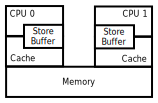
\includegraphics{memorder/SystemArchSB}}
\caption{System Architecture With Store Buffers}
\label{fig:memorder:System Architecture With Store Buffers}
\end{figure}

CPUs therefore come equipped with store buffers, as shown in
\cref{fig:memorder:System Architecture With Store Buffers}.
When a given CPU stores to a variable
not present in that CPU's cache, then the new value
is instead placed in that CPU's store buffer.
The CPU can then proceed immediately, without having to wait for the
store to do something about all the old values of that variable
residing in other CPUs' caches.

\begin{figure}[tb]
\centering
\resizebox{2.4in}{!}{\includegraphics{cartoons/r-2014-Out-of-order}}
\caption{CPUs Can Do Things Out of Order}
\ContributedBy{Figure}{fig:memorder:CPUs Can Do Things Out of Order}{Melissa Broussard}
\end{figure}

Although store buffers can greatly increase performance,
they can cause instructions and memory references to execute out
of order, which can in turn cause serious confusion, as illustrated in
\cref{fig:memorder:CPUs Can Do Things Out of Order}.
In particular, these store buffers cause the memory misordering
shown in the store-buffering litmus test in
\cref{lst:memorder:Memory Misordering: Store-Buffering Litmus Test}.

\begin{table*}[tbh]
\rowcolors{6}{}{lightgray}
\renewcommand*{\arraystretch}{1.1}
\small
\centering\OneColumnHSpace{-0.1in}
\begin{tabular}{rllllll}
	\toprule
	& \multicolumn{3}{c}{CPU 0} & \multicolumn{3}{c}{CPU 1} \\
	\cmidrule(l){2-4} \cmidrule(l){5-7}
	& Instruction & Store Buffer & Cache &
		Instruction & Store Buffer & Cache \\
	\cmidrule{1-1} \cmidrule(l){2-4} \cmidrule(l){5-7}
	1 & (Initial state) & & \tco{x1==0} &
		(Initial state) & & \tco{x0==0} \\
	2 & \tco{x0 = 2;} & \tco{x0==2} & \tco{x1==0} &
		\tco{x1 = 2;} & \tco{x1==2} & \tco{x0==0} \\
	3 & \tco{r2 = x1;} (0) & \tco{x0==2} & \tco{x1==0} &
		\tco{r2 = x0;} (0) & \tco{x1==2} & \tco{x0==0} \\
	4 & (Read-invalidate) & \tco{x0==2} & \tco{x0==0} &
		(Read-invalidate) & \tco{x1==2} & \tco{x1==0} \\
	5 & (Finish store) & & \tco{x0==2} &
		(Finish store) & & \tco{x1==2} \\
	\bottomrule
\end{tabular}
\caption{Memory Misordering: Store-Buffering Sequence of Events}
\label{tab:memorder:Memory Misordering: Store-Buffering Sequence of Events}
\end{table*}

\Cref{tab:memorder:Memory Misordering: Store-Buffering Sequence of Events}
shows how this memory misordering can happen.
Row~1 shows the initial state, where CPU~0 has \co{x1} in its cache
and CPU~1 has \co{x0} in its cache, both variables having a value of zero.
\begin{lineref}[ln:formal:C-SB+o-o+o-o:whole]
Row~2 shows the state change due to each CPU's store (\clnref{st0,st1} of
\cref{lst:memorder:Memory Misordering: Store-Buffering Litmus Test}).
Because neither CPU has the stored-to variable in its cache, both CPUs
record their stores in their respective store buffers.
\end{lineref}

\QuickQuiz{}
	But wait!!!
	On row~2 of
	\cref{tab:memorder:Memory Misordering: Store-Buffering Sequence of Events}
	both \co{x0} and \co{x1} each have two values at the same time,
	namely zero and two.
	How can that possibly work???
\QuickQuizAnswer{
	There is an underlying cache-coherence protocol that straightens
	things out, which are discussed in
	\cref{sec:app:whymb:Cache-Coherence Protocols}.
	But if you think that a given variable having two values at
	the same time is surprising, just wait until you get to
	\cref{sec:memorder:Variables With Multiple Values}!
} \QuickQuizEnd

\begin{lineref}[ln:formal:C-SB+o-o+o-o:whole]
Row~3 shows the two loads (\clnref{ld0,ld1} of
\cref{lst:memorder:Memory Misordering: Store-Buffering Litmus Test}).
Because the variable being loaded by each CPU is in that CPU's cache,
each load immediately returns the cached value, which in both cases
is zero.
\end{lineref}

But the CPUs are not done yet: Sooner or later, they must empty their
store buffers.
Because caches move data around in relatively large blocks called
\emph{cachelines}, and because each cacheline can hold several
variables, each CPU must get the cacheline into its own cache so
that it can update the portion of that cacheline corresponding
to the variable in its store buffer, but without disturbing any
other part of the cacheline.
Each CPU must also ensure that the cacheline is not present in any other
CPU's cache, for which a read-invalidate operation is used.
As shown on row~4, after both read-invalidate operations complete,
the two CPUs have traded cachelines, so that CPU~0's cache now contains
\co{x0} and CPU~1's cache now contains \co{x1}.
Once these two variables are in their new homes, each CPU can flush
its store buffer into the corresponding cache line, leaving each
variable with its final value as shown on row~5.

\QuickQuiz{}
	But don't the values also need to be flushed from the cache
	to main memory?
\QuickQuizAnswer{
	Perhaps surprisingly, not necessarily!
	On some systems,
	if the two variables are being used heavily, they might
	be bounced back and forth between the CPUs' caches and never
	land in main memory.
} \QuickQuizEnd

In summary, store buffers are needed to allow CPUs to handle
store instructions efficiently, but they can result in
counter-intuitive memory misordering.

But what do you do if your algorithm really needs its memory
references to be ordered?
For example, suppose that you are communicating with a driver using
a pair of flags, one that says whether or not the driver is running
and the other that says whether there is a request pending for that
driver.
The requester needs to set the request-pending flag, then check
the driver-running flag, and if false, wake the driver.
Once the driver has serviced all the pending requests that it knows about,
it needs to clear its driver-running flag, then check the request-pending
flag to see if it needs to restart.
This very reasonable approach cannot work unless there is some way
to make sure that the hardware processes the stores and loads in order.
This is the subject of the next section.

\subsection{How to Force Ordering?}
\label{sec:memorder:How to Force Ordering?}

It turns out that there are compiler directives and standard
synchronization primitives (such as locking and RCU)
that are responsible for maintaining the illusion of ordering through use of
\emph{memory barriers} (for example, \co{smp_mb()} in the Linux kernel).
These memory barriers can be explicit instructions, as they are on
ARM, \Power{}, Itanium, and Alpha, or they can be implied by other instructions,
as they often are on x86.
Since these standard synchronization primitives preserve the illusion of
ordering, your path of least resistance is to simply use these primitives,
thus allowing you to stop reading this section.

\begin{listing}[tbp]
\input{CodeSamples/formal/litmus/C-SB+o-mb-o+o-mb-o@whole.fcv}
\caption{Memory Ordering: Store-Buffering Litmus Test}
\label{lst:memorder:Memory Ordering: Store-Buffering Litmus Test}
\end{listing}

However, if you need to implement the synchronization primitives
themselves, or if you are simply interested in understanding how memory
ordering works, read on!
The first stop on the journey is
\cref{lst:memorder:Memory Ordering: Store-Buffering Litmus Test}
(\path{C-SB+o-mb-o+o-mb-o.litmus}),
which places an \co{smp_mb()} Linux-kernel full memory barrier between
the store and load in both \co{P0()} and \co{P1()}, but is otherwise
identical to
\cref{lst:memorder:Memory Misordering: Store-Buffering Litmus Test}.
% Test C-SB+o-mb-o+o-mb-o Allowed
% Histogram (3 states)
% 49553298:>0:r2=2; 1:r2=0;
% 49636449:>0:r2=0; 1:r2=2;
% 810253:>0:r2=2; 1:r2=2;
% No
These barriers prevent the counter-intuitive outcome from happening
on 100,000,000 trials on my x86 laptop.
Interestingly enough, the added overhead due to these barriers causes the
legal outcome where both loads return the value two to happen more
than 800,000 times, as opposed to only 167 times for the
barrier-free code in
\cref{lst:memorder:Memory Misordering: Store-Buffering Litmus Test}.

\begin{table*}[tbh]
\rowcolors{6}{}{lightgray}
\renewcommand*{\arraystretch}{1.1}
\small
\centering\OneColumnHSpace{-0.1in}
\begin{tabular}{rllllll}
	\toprule
	& \multicolumn{3}{c}{CPU 0} & \multicolumn{3}{c}{CPU 1} \\
	\cmidrule(l){2-4} \cmidrule(l){5-7}
	& Instruction & Store Buffer & Cache &
		Instruction & Store Buffer & Cache \\
	\cmidrule{1-1} \cmidrule(l){2-4} \cmidrule(l){5-7}
	1 & (Initial state) & & \tco{x1==0} &
		(Initial state) & & \tco{x0==0} \\
	2 & \tco{x0 = 2;} & \tco{x0==2} & \tco{x1==0} &
		\tco{x1 = 2;} & \tco{x1==2} & \tco{x0==0} \\
	3 & \tco{smp_mb();} & \tco{x0==2} & \tco{x1==0} &
		\tco{smp_mb();} & \tco{x1==2} & \tco{x0==0} \\
	4 & (Read-invalidate) & \tco{x0==2} & \tco{x0==0} &
		(Read-invalidate) & \tco{x1==2} & \tco{x1==0} \\
	5 & (Finish store) & & \tco{x0==2} &
		(Finish store) & & \tco{x1==2} \\
	6 & \tco{r2 = x1;} (2) & & \tco{x1==2} &
		\tco{r2 = x0;} (2) & & \tco{x0==2} \\
	\bottomrule
\end{tabular}
\caption{Memory Ordering: Store-Buffering Sequence of Events}
\label{tab:memorder:Memory Ordering: Store-Buffering Sequence of Events}
\end{table*}

These barriers have a profound effect on ordering, as can be seen in
\cref{tab:memorder:Memory Ordering: Store-Buffering Sequence of Events}.
Although the first two rows are the same as in
\cref{tab:memorder:Memory Misordering: Store-Buffering Sequence of Events}
and although the \co{smp_mb()} instructions on row~3
do not change state
in and of themselves, they do cause the stores to complete
(rows~4 and~5) before the
loads (row~6), which rules out the counter-intuitive outcome shown in
\cref{tab:memorder:Memory Misordering: Store-Buffering Sequence of Events}.
Note that variables \co{x0} and \co{x1} each still have more than one
value on row~2, however, as promised earlier, the \co{smp_mb()}
instances straighten things out in the end.

Although full barriers such as \co{smp_mb()} have extremely strong
ordering guarantees, their strength comes at a high price.
A great many situations can be handled with much weaker ordering guarantees
that use much cheaper memory-ordering instructions, or, in some case, no
memory-ordering instructions at all.

\begin{table*}[tbh]
\small
\centering\OneColumnHSpace{-0.7in}
\renewcommand*{\arraystretch}{1.1}
\rowcolors{7}{lightgray}{}
\begin{tabular}{lcccccccccccc}\toprule
	& & \multicolumn{4}{c}{Prior Ordered Operation} &
		\multicolumn{7}{c}{Subsequent Ordered Operation} \\
	\cmidrule(l){3-6} \cmidrule(l){7-13}
	Operation Providing Ordering & C &
		Self & R & W & RMW & Self & R & W & DR & DW & RMW & SV \\
	\cmidrule(r){1-1} \cmidrule{2-2} \cmidrule(l){3-6} \cmidrule(l){7-13}
	Store, for example, \tco{WRITE_ONCE()} &  &
		   Y &   &   &     &      &   &   &    &    &     &  Y \\
	Load, for example, \tco{READ_ONCE()} &  &
		   Y &   &   &     &      &   &   &  Y &  Y &     &  Y \\
	\tco{_relaxed()} RMW operation &  &
		   Y &   &   &     &      &   &   &  Y &  Y &     &  Y \\
	\tco{smp_read_barrier_depends()} &  &
		     & Y &   &     &      &   &   &  Y &  Y &     &    \\
	\tco{*_dereference()} &  &
		   Y &   &   &     &      &   &   &  Y &  Y &     &  Y \\
	Successful \tco{*_acquire()} &   &
		   R &   &   &     &      & Y & Y &  Y &  Y &   Y &  Y \\
	Successful \tco{*_release()} & C &
		     & Y & Y &   Y &    W &   &   &    &    &     &  Y \\
	\tco{smp_rmb()} &   &
		     & Y &   &   R &      & Y &   &  Y &    &   R &    \\
	\tco{smp_wmb()} &   &
		     &   & Y &   W &      &   & Y &    &  Y &   W &    \\
	\tco{smp_mb()} and \tco{synchronize_rcu()} & CP &
		     & Y & Y &   Y &      & Y & Y &  Y &  Y &   Y &    \\
	Successful full-strength non-\tco{void} RMW & CP &
		   Y & Y & Y &   Y &    Y & Y & Y &  Y &  Y &   Y &  Y \\
	\tco{smp_mb__before_atomic()} & CP &
		     & Y & Y &   Y &      & a & a & a  & a  &   Y &    \\
	\tco{smp_mb__after_atomic()} & CP &
		     & a & a &   Y &      & Y & Y &  Y &  Y &   Y &    \\
	\bottomrule
\end{tabular}

\vspace{5pt}\hfill
\framebox[\width]{\footnotesize\setlength{\tabcolsep}{3pt}
\rowcolors{1}{}{}
\begin{tabular}{lrl}
	Key:	& C: & Ordering is cumulative \\
		& P: & Ordering propagates \\
		& R: & Read, for example, \tco{READ_ONCE()}, or read portion of RMW \\
		& W: & Write, for example, \tco{WRITE_ONCE()}, or write portion of RMW \\
		& Y: & Provides the specified ordering \\
		& a: & Provides specified ordering given intervening RMW atomic operation \\
		& DR: & Dependent read (address dependency, \cref{sec:memorder:Address Dependencies}) \\
		& DW: & Dependent write (address, data, or control dependency, \crefrange{sec:memorder:Address Dependencies}{sec:memorder:Control Dependencies}) \\
		& RMW: & Atomic read-modify-write operation \\
		& Self: & Orders self, as opposed to accesses both before
			  and after \\
		& SV: & Orders later accesses to the same variable \\
	\multicolumn{3}{l}{\emph{Applies to Linux kernel v4.15 and later.}} \\
\end{tabular}
}\OneColumnHSpace{-0.9in}
\caption{Linux-Kernel Memory-Ordering Cheat Sheet}
\label{tab:memorder:Linux-Kernel Memory-Ordering Cheat Sheet}
\end{table*}

\Cref{tab:memorder:Linux-Kernel Memory-Ordering Cheat Sheet}
provides a cheatsheet of the Linux kernel's ordering primitives and their
guarantees.
Each row corresponds to a primitive or category of primitives that might
or might not provide ordering, with the columns labeled
``Prior Ordered Operation'' and ``Subsequent Ordered Operation''
being the operations that might (or might not) be ordered against.
Cells containing ``Y'' indicate that ordering is supplied unconditionally,
while other characters indicate that ordering is supplied only partially or
conditionally.
Blank cells indicate that no ordering is supplied.

The ``Store'' row also covers the store portion of an atomic RMW operation.
In addition, the ``Load'' row covers the load
component of a successful value-returning \co{_relaxed()} RMW atomic
operation, although the combined ``\co{_relaxed()} RMW operation''
line provides a convenient combined reference in the value-returning case.
A CPU executing unsuccessful value-returning atomic RMW operations must
invalidate the corresponding variable from all other CPUs' caches.
Therefore, oddly enough, unsuccessful value-returning atomic RMW
operations have many of the properties of a store, which means that the
``\co{_relaxed()} RMW operation'' line also applies to unsuccessful
value-returning atomic RMW operations.

The \co{*_acquire} row covers \co{smp_load_acquire()},
\co{cmpxchg_acquire()}, \co{xchg_acquire()}, and so on;
the \co{*_release} row covers \co{smp_store_release()},
\co{cmpxchg_release()}, \co{xchg_release()}, and so on; and
the ``Successful full-strength non-\co{void} RMW'' row covers
\co{atomic_add_return()}, \co{atomic_add_unless()}, \co{atomic_dec_and_test()},
\co{cmpxchg()}, \co{xchg()}, and so on.
The ``Successful'' qualifiers apply to primitives such as
\co{atomic_add_unless()}, \co{cmpxchg_acquire()}, and \co{cmpxchg_release()},
which have no effect on either memory or on ordering when they indicate
failure, as indicated by the earlier ``\co{_relaxed()} RMW operation'' row.

Column ``C'' indicates cumulativity and propagation, as explained in
\cref{sec:memorder:Cumulativity,sec:memorder:Propagation}.
In the meantime, this column can usually be ignored when there
are at most two threads involved.

\QuickQuiz{}
	The rows in
	\cref{tab:memorder:Linux-Kernel Memory-Ordering Cheat Sheet}
	seem quite random and confused.
	Whatever is the conceptual basis of this table???
\QuickQuizAnswer{
	The rows correspond roughly to hardware mechanisms of increasing
	power and overhead.

	The \co{WRITE_ONCE()} row captures the fact that accesses to
	a single variable are always fully ordered, as indicated by
	the ``SV''column.
	Note that all other operations providing ordering against accesses
	to multiple variables also provide this same-variable ordering.

	The \co{READ_ONCE()} row captures the fact that (as of 2018) compilers
	and CPUs do not indulge in user-visible speculative stores, so that
	any store whose address, data, or execution depends on a prior load
	is guaranteed to happen after that load completes.
	However, this guarantee assumes that these dependencies have
	been constructed carefully as described in
	\cref{sec:memorder:Address- and Data-Dependency Difficulties,%
	sec:memorder:Control-Dependency Calamities}.

	The ``\co{_relaxed()} RMW operation'' row captures the fact
	that a value-returning \co{_relaxed()} RMW has done a load and a
	store, which are every bit as good as a \co{READ_ONCE()} and a
	\co{WRITE_ONCE()}, respectively.

	The \co{smp_read_barrier_depends()} row captures the fact that, with the
	notable exception of DEC Alpha, compilers and CPUs do not indulge
	in user-visible breakage of address dependencies, again assuming
	that these dependencies have been constructed carefully as described in
	\cref{sec:memorder:Address- and Data-Dependency Difficulties}.
	However, as of version v4.15 of the Linux kernel, the fact that
	\co{READ_ONCE()} provides dependency ordering should mean that
	there is little further need for \co{smp_read_barrier_depends()}.

	The \co{*_dereference()} row captures the address and data
	dependency ordering provided by \co{rcu_dereference()} and friends.

	The ``Successful \co{*_acquire()}'' row captures the fact that many
	CPUs have special ``acquire'' forms of loads and of atomic RMW
	instructions,
	and that many other CPUs have lightweight memory-barrier
	instructions that order prior loads against subsequent loads
	and stores.

	The ``Successful \co{*_release()}'' row captures the fact that many
	CPUs have special ``release'' forms of stores and of atomic RMW
	instructions, and that many other CPUs have lightweight memory-barrier
	instructions that order prior loads and stores against
	subsequent stores.

	The \co{smp_rmb()} row captures the fact that many CPUs have
	lightweight memory-barrier instructions that order prior loads against
	subsequent loads.
	Similarly,
	the \co{smp_wmb()} row captures the fact that many CPUs have
	lightweight memory-barrier instructions that order prior stores against
	subsequent stores.

	None of the ordering operations thus far require prior stores to be
	ordered against subsequent loads, which means that these operations
	need not interfere with store buffers, whose main purpose in life
	is in fact to reorder prior stores against subsequent loads.
	The lightweight nature of these operations is precisely due to
	their policy of store-buffer non-interference.
	However, as noted earlier, it is sometimes necessary to interfere
	with the store buffer in order to prevent prior stores from being
	reordered against later stores, which brings us to the remaining
	rows in this table.

	The \co{smp_mb()} row corresponds to the full memory barrier
	available on most platforms, with Itanium being the exception
	that proves the rule.
	However, even on Itanium, \co{smp_mb()} provides full ordering
	with respect to \co{READ_ONCE()} and \co{WRITE_ONCE()},
	as discussed in \cref{sec:memorder:Itanium}.

	The ``Successful full-strength non-\co{void} RMW'' row captures
	the fact that on some platforms (such as x86) atomic RMW instructions
	provide full ordering both before and after.
	The Linux kernel therefore requires that full-strength non-\co{void}
	atomic RMW operations provide full ordering in cases where these
	operations succeed.
	(Full-strength atomic RMW operation's names do not end in
	\co{_relaxed}, \co{_acquire}, or \co{_release}.)
	As noted earlier, the case where these operations do not succeed
	is covered by the ``\co{_relaxed()} RMW operation'' row.

	However, the Linux kernel does not require that either \co{void}
	or \co{_relaxed()} atomic RMW operations provide any ordering
	whatsoever, with the canonical example being \co{atomic_inc()}.
	Therefore, these operations, along with failing non-\co{void}
	atomic RMW operations may be preceded by \co{smp_mb__before_atomic()}
	and followed by \co{smp_mb__after_atomic()} to provide full
	ordering for any accesses preceding or following both.
	No ordering need be provided for accesses between the
	\co{smp_mb__before_atomic()} (or, similarly, the
	\co{smp_mb__after_atomic()}) and the atomic RMW operation, as
	indicated by the ``a'' entries on the \co{smp_mb__before_atomic()}
	and \co{smp_mb__after_atomic()} rows of the table.

	In short, any randomness in the table is due to the properties
	of the underlying hardware, which are constrained by nothing other
	than the laws of physics, which were covered back in
	\cref{chp:Hardware and its Habits}.
} \QuickQuizEnd

\QuickQuiz{}
	Why is
	\cref{tab:memorder:Linux-Kernel Memory-Ordering Cheat Sheet}
	missing \co{smp_mb__after_unlock_lock()} and
	\co{smp_mb__after_spinlock()}?
\QuickQuizAnswer{
	These two primitives are rather specialized, and at present
	seem difficult to fit into 
	\cref{tab:memorder:Linux-Kernel Memory-Ordering Cheat Sheet}.
	The \co{smp_mb__after_unlock_lock()} primitive is intended to be placed
	immediately after a lock acquisition, and ensures that all CPUs
	see all accesses in prior critical sections as happening before
	all accesses following the \co{smp_mb__after_unlock_lock()}
	and also before all accesses in later critical sections.
	Here ``all CPUs'' includes those CPUs not holding that lock,
	and ``prior critical sections'' includes all prior critical sections
	for the lock in question as well as all prior critical sections
	for all other locks that were released by the same CPU that executed
	the  \co{smp_mb__after_unlock_lock()}.

	The \co{smp_mb__after_spinlock()} provides the same guarantees
	as does \co{smp_mb__after_unlock_lock()}, but also provides
	additional visibility guarantees for other accesses performed
	by the CPU that executed the \co{smp_mb__after_spinlock()}.
	Given any store S performed prior to any earlier lock acquisition
	and any load L performed after the \co{smp_mb__after_spinlock()},
	all CPUs will see S as happening before L.
	In other words, if a CPU performs a store S, acquires a lock,
	executes an \co{smp_mb__after_spinlock()}, then performs a
	load L, all CPUs will see S as happening before L.
} \QuickQuizEnd

It is important to note that this table is just a cheat sheet,
and is therefore in no way a replacement for a good understanding
of memory ordering.
To begin building such an understanding, the next section will
present some basic rules of thumb.

\subsection{Basic Rules of Thumb}
\label{sec:memorder:Basic Rules of Thumb}

This section presents some basic rules of thumb that are ``good and
sufficient'' for a great many situations.
In fact, you could write a great deal of concurrent code having
excellent performance and scalability without needing anything more
than these rules of thumb.

\QuickQuiz{}
	But how can I know that a given project can be designed
	and coded within the confines of these rules of thumb?
\QuickQuizAnswer{
	Much of the purpose of the remainder of this chapter is
	to answer exactly that question!
} \QuickQuizEnd

\paragraph{A given thread sees its own accesses in order.}
This rule assumes that loads and stores from/to shared variables use
\co{READ_ONCE()} and \co{WRITE_ONCE()}, respectively.
Otherwise, the compiler can profoundly scramble\footnote{
	Compiler writers often prefer the word ``optimize''.}
your code, and sometimes the CPU can do a bit of scrambling as well
(as is discussed in \cref{sec:memorder:Itanium}).

\begin{figure}[tb]
\centering
\resizebox{3in}{!}{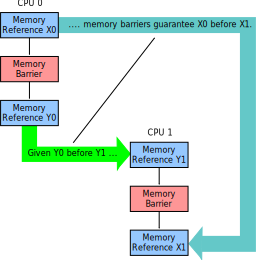
\includegraphics{memorder/memorybarrier}}
\caption{Memory Barriers Provide Conditional If-Then Ordering}
\label{fig:memorder:Memory Barriers Provide Conditional If-Then Ordering}
\end{figure}

\paragraph{Ordering has conditional if-then semantics.}
\Cref{fig:memorder:Memory Barriers Provide Conditional If-Then Ordering}
illustrates this for memory barriers.
Assuming that both memory barriers are strong enough (and when in doubt, you
can always use \co{smp_mb()}), if CPU~1's access Y1 happens after CPU~0's
access Y0, then CPU~1's access X1 is guaranteed to happen after CPU~0's
access X1.

\QuickQuiz{}
	How can you tell which memory barriers are strong enough for
	a given use case?
\QuickQuizAnswer{
	Ah, that is a deep question whose answer requires most of the
	rest of this chapter.
} \QuickQuizEnd

\begin{lineref}[ln:formal:C-SB+o-mb-o+o-mb-o:whole]
\Cref{lst:memorder:Memory Ordering: Store-Buffering Litmus Test}
is a case in point.
The \co{smp_mb()} on \clnref{P0:mb,P1:mb} serve as the barriers,
the store to \co{x0} on \clnref{P0:st} as X0, the load from \co{x1}
on \clnref{P0:ld} as Y0, the store to \co{x1} on \clnref{P1:st} as Y1,
and the load from \co{x0} as X1.
Applying the if-then rule step by step, we know that the store to
\co{x1} on \clnref{P1:st} happens after the load from \co{x1} on \clnref{P0:ld} if
\co{P0()}'s local variable \co{r2} is set to the value zero.
The if-then rule would then state that the load from \co{x0} on
\clnref{P1:ld} happens after the store to \co{x0} on \clnref{P0:st}.
In other words,
\co{P1()}'s local variable \co{r2} is guaranteed
to end up with the value two \emph{only if}
\co{P0()}'s local variable \co{r2} ends up with the value zero.
This underscores the point that memory ordering guarantees are
conditional, not absolute.
\end{lineref}

Although
\cref{fig:memorder:Memory Barriers Provide Conditional If-Then Ordering}
specifically mentions memory barriers, the same rule applies to the
rest of the Linux kernel's ordering operations.

\paragraph{Ordering operations must be paired.}
If you carefully order the operations in one thread, but then fail to do
so in another thread, then there is no ordering.
Both threads must provide ordering for the if-then rule to apply.\footnote{
	In \cref{sec:memorder:Propagation}, pairing will be
	generalized to cycles.}

\paragraph{Ordering operations almost never speed things up.}
If you find yourself tempted to add a memory barrier in an attempt
to force a prior store to be flushed to memory faster, resist!
Adding ordering usually slows things down.
Of course, there are situations where adding instructions speeds things
up, but careful benchmarking is required in such cases.
And even then, it is quite possible that although you sped things up
a little bit on \emph{your} system, you might well have slowed things
down significantly on your users' systems.
Or on your future system.

\paragraph{Ordering operations are not magic.}
When your program is failing due to some race condition, it is often
tempting to toss in a few memory-ordering operations in an attempt
to barrier your bugs out of existence.
A far better reaction is to use higher-level primitives in a carefully
designed manner.
With concurrent programming, it is almost always easier to design
your bugs out of existence than to hack them out of existence!

\paragraph{These are only rough rules of thumb.}
Although these rules of thumb cover the vast majority of situations
seen in actual practice, as with any set of rules of thumb, they
do have their limits.
The next section will demonstrate some of these limits by introducing
trick-and-trap litmus tests that are intended to insult your
intuition while increasing your understanding.
These litmus tests will also illuminate many of the concepts
represented by the Linux-kernel memory-ordering cheat sheet shown in
\cref{tab:memorder:Linux-Kernel Memory-Ordering Cheat Sheet},
and can be automatically analyzed given proper
tooling~\cite{Alglave:2018:FSC:3173162.3177156}.
\Cref{sec:memorder:Where is Memory Ordering Needed?} will
circle back to this cheat sheet, presenting a more sophisicated set of
rules of thumb in light of learnings from all the intervening tricks
and traps.

\QuickQuiz{}
	Wait!!!
	Where do I find this tooling that automatically analyzes
	litmus tests???
\QuickQuizAnswer{
	Get version v4.17 (or later) of the Linux-kernel source code,
	then follow the instructions in \path{tools/memory-model/README}
	to install the needed tools.
	Then follow the further instructions to run these tools on the
	litmus test of your choice.
} \QuickQuizEnd

\section{Tricks and Traps}
\label{sec:memorder:Tricks and Traps}

Now that you know that hardware can reorder memory accesses and that you
can prevent it from doing so, the next step is to get you to admit
that your intuition has a problem.
This painful task is taken up by
\cref{sec:memorder:Variables With Multiple Values},
which presents some code demonstrating that scalar variables can
take on multiple values simultaneously,
and by
\crefthro{sec:memorder:Memory-Reference Reordering}
{sec:memorder:Multicopy Atomicity},
which show a series of intuitively correct code fragments that fail miserably
on real hardware.
Once your intuition has made it through the grieving process, later
sections will summarize the basic rules that memory ordering follows.

But first, let's take a quick look at just how many values a single
variable might have at a single point in time.

\subsection{Variables With Multiple Values}
\label{sec:memorder:Variables With Multiple Values}

It is natural to think of a variable as taking on a well-defined
sequence of values in a well-defined, global order.
Unfortunately, the next stop on the journey says ``goodbye'' to this comforting fiction.
Hopefully, you already started to say ``goodbye'' in response to row~2 of
\cref{tab:memorder:Memory Misordering: Store-Buffering Sequence of Events,%
tab:memorder:Memory Ordering: Store-Buffering Sequence of Events},
and if so, the purpose of this section is to drive this point home.

\begin{lineref}[ln:memorder:Software Logic Analyzer]
To this end, consider the program fragment shown in
\cref{lst:memorder:Software Logic Analyzer}.
This code fragment is executed in parallel by several CPUs.
\Clnref{setid} sets a shared variable to the current CPU's ID, \clnref{init}
initializes several variables from a \co{gettb()} function that
delivers the value of a fine-grained hardware ``timebase'' counter that is
synchronized among all CPUs (not available from all CPU architectures,
unfortunately!), and the loop from \clnrefrange{loop:b}{loop:e}
records the length of
time that the variable retains the value that this CPU assigned to it.
Of course, one of the CPUs will ``win'', and would thus never exit
the loop if not for the check on \clnrefrange{iftmout}{break}.
\end{lineref}

\QuickQuiz{}
	What assumption is the code fragment
	in \cref{lst:memorder:Software Logic Analyzer}
	making that might not be valid on real hardware?
\QuickQuizAnswer{
	The code assumes that as soon as a given CPU stops
	seeing its own value, it will immediately see the
	final agreed-upon value.
	On real hardware, some of the CPUs might well see several
	intermediate results before converging on the final value.
	The actual code used to produce the data in the figures
	discussed later in this section was therefore somewhat more
	complex.
} \QuickQuizEnd

\begin{listing}[tbp]
\begin{linelabel}[ln:memorder:Software Logic Analyzer]
\begin{VerbatimL}[commandchars=\\\[\]]
state.variable = mycpu;			\lnlbl[setid]
lasttb = oldtb = firsttb = gettb();	\lnlbl[init]
while (state.variable == mycpu) {	\lnlbl[loop:b]
	lasttb = oldtb;
	oldtb = gettb();
	if (lasttb - firsttb > 1000)	\lnlbl[iftmout]
		break;			\lnlbl[break]
}					\lnlbl[loop:e]
\end{VerbatimL}
\end{linelabel}
\caption{Software Logic Analyzer}
\label{lst:memorder:Software Logic Analyzer}
\end{listing}

Upon exit from the loop, \co{firsttb} will hold a timestamp
taken shortly after the assignment and \co{lasttb} will hold
a timestamp taken before the last sampling of the shared variable
that still retained the assigned value, or a value equal to \co{firsttb}
if the shared variable had changed before entry into the loop.
This allows us to plot each CPU's view of the value of \co{state.variable}
over a 532-nanosecond time period, as shown in
\cref{fig:memorder:A Variable With Multiple Simultaneous Values}.
This data was collected in 2006 on 1.5\,GHz \Power{5} system with 8 cores,
each containing a pair of hardware threads.
CPUs~1, 2, 3, and~4 recorded the values, while CPU~0 controlled the test.
The timebase counter period was about 5.32\,ns, sufficiently fine-grained
to allow observations of intermediate cache states.

\begin{figure}[htb]
\centering
\resizebox{3in}{!}{\includegraphics{memorder/MoreThanOneValue}}
\caption{A Variable With Multiple Simultaneous Values}
\label{fig:memorder:A Variable With Multiple Simultaneous Values}
\end{figure}

Each horizontal bar represents the observations of a given CPU over time,
with the gray regions to the left indicating the time before the
corresponding CPU's first measurement.
During the first 5\,ns, only CPU~3 has an opinion about the value of the
variable.
During the next 10\,ns, CPUs~2 and~3 disagree on the value of the variable,
but thereafter agree that the value is~``2'', which is in fact
the final agreed-upon value.
However, CPU~1 believes that the value is~``1'' for almost 300\,ns, and
CPU~4 believes that the value is~``4'' for almost 500\,ns.

\QuickQuiz{}
	How could CPUs possibly have different views of the
	value of a single variable \emph{at the same time?}
\QuickQuizAnswer{
	As discussed in
	\cref{sec:memorder:Why Hardware Misordering?},
	many CPUs have store buffers that record the values of
	recent stores, which do not become globally visible until
	the corresponding cache line makes its way to the CPU.
	Therefore, it is quite possible for each CPU to see a
	different value for a given variable at a single point
	in time---and for main memory to hold yet another value.
	One of the reasons that memory barriers were invented was
	to allow software to deal gracefully with situations like
	this one.
} \QuickQuizEnd

\QuickQuiz{}
	Why do CPUs~2 and~3 come to agreement so quickly, when it
	takes so long for CPUs~1 and~4 to come to the party?
\QuickQuizAnswer{
	CPUs~2 and~3 are a pair of hardware threads on the same
	core, sharing the same cache hierarchy, and therefore have
	very low communications latencies.
	This is a NUMA, or, more accurately, a NUCA effect.

	This leads to the question of why CPUs~2 and~3 ever disagree
	at all.
	One possible reason is that they each might have a small amount
	of private cache in addition to a larger shared cache.
	Another possible reason is instruction reordering, given the
	short 10-nanosecond duration of the disagreement and the
	total lack of memory-ordering operations in the code fragment.
} \QuickQuizEnd

And if you think that the situation with four CPUs was intriguing, consider
\cref{fig:memorder:A Variable With More Simultaneous Values},
which shows the same situation, but with 15~CPUs each assigning their
number to a single shared variable at time~$t=0$. Both diagrams in the
figure are drawn in the same way as
\cref{fig:memorder:A Variable With Multiple Simultaneous Values}.
The only difference is that the unit of horizontal axis is timebase ticks,
with each tick lasting about 5.3~nanoseconds.
The entire sequence therefore lasts a bit longer than the events recorded in
\cref{fig:memorder:A Variable With Multiple Simultaneous Values},
consistent with the increase in number of CPUs.
The upper diagram shows the overall picture, while the lower one shows
the zoom-up of first 50~timebase ticks.

Again, CPU~0 coordinates the test, so does not record any values.

\begin{figure*}
\centering
\resizebox{5in}{!}{\includegraphics{memorder/MoreThanOneValue-15CPU}}
\caption{A Variable With More Simultaneous Values}
\ContributedBy{Figure}{fig:memorder:A Variable With More Simultaneous Values}{Akira Yokosawa}
\end{figure*}

All CPUs eventually agree on the final value of~9, but not before
the values~15 and~12 take early leads.
Note that there are fourteen different opinions on the variable's value
at time~21 indicated by the vertical line in the lower diagram.
Note also that all CPUs see sequences whose orderings are consistent with
the directed graph shown in
\cref{fig:memorder:Possible Global Orders With More Simultaneous Values}.
Nevertheless, both figures underscore the importance of
proper use of memory-ordering operations, such as memory barriers,
for code that cares about memory ordering.

\begin{figure}[htb]
\centering
\resizebox{2.0in}{!}{\includegraphics{memorder/store15tred}}
\caption{Possible Global Orders With More Simultaneous Values}
\label{fig:memorder:Possible Global Orders With More Simultaneous Values}
\end{figure}

How many values can a single variable take on at a single point in
time?
As many as one per store buffer in the system!
We have therefore entered a regime where we must bid a fond farewell to
comfortable intuitions about values of variables and the passage of time.
This is the regime where memory-ordering operations are needed.

All that aside, it is important to remember the lessons from
\cref{chp:Hardware and its Habits,%
cha:Partitioning and Synchronization Design}.
Having all CPUs store concurrently to the same variable
is absolutely no way to design a parallel program, at least
not if performance and scalability are at all important to you.

Unfortunately, memory ordering has many other ways of insulting your
intuition, and not all of these ways conflict with performance and
scalability.
The next section overviews reordering of unrelated memory reference.

\subsection{Memory-Reference Reordering}
\label{sec:memorder:Memory-Reference Reordering}

\Cref{sec:memorder:Why Hardware Misordering?}
showed that even relatively strongly ordered systems like x86
can reorder prior stores with later loads, at least when the
store and load are to different variables.
This section builds on that result, looking at the other combinations of
loads and stores.

\begin{listing}[tbp]
\input{CodeSamples/formal/litmus/C-MP+o-wmb-o+o-o@whole.fcv}
\caption{Message-Passing Litmus Test (No Ordering)}
\label{lst:memorder:Message-Passing Litmus Test (No Ordering)}
\end{listing}

\subsubsection{Load Followed By Load}
\label{sec:memorder:Load Followed By Load}

\begin{lineref}[ln:formal:C-MP+o-wmb-o+o-o:whole]
\Cref{lst:memorder:Message-Passing Litmus Test (No Ordering)}
(\path{C-MP+o-wmb-o+o-o.litmus})
shows the classic \emph{message-passing} litmus test, where \co{x0} is
the message and \co{x1} is a flag indicating whether or not a message
is available.
In this test, the \co{smp_wmb()} forces \co{P0()} stores to be ordered,
but no ordering is specified for the loads.
Relatively strongly ordered architectures, such as x86, do enforce ordering.
However, weakly ordered architectures often do
not~\cite{JadeAlglave2011ppcmem}.
Therefore, the \co{exists} clause on \clnref{exists} of the listing \emph{can}
trigger.
\end{lineref}

One rationale for reordering loads from different locations is that doing
so allows execution to proceed when an earlier load misses the cache,
but the values for later loads are already present.

\QuickQuiz{}
	But why make load-load reordering visible to the user?
	Why not just use speculative execution to allow execution to
	proceed in the common case where there are no intervening
	stores, in which case the reordering cannot be visible anyway?
\QuickQuizAnswer{
	They can and many do, otherwise systems containing
	strongly ordered CPUs would be slow indeed.
	However, speculative execution does have its downsides, especially
	if speculation must be rolled back frequently, and especially
	on battery-powered systems.
	But perhaps future systems will be able to overcome these
	disadvantages.
	Until then, we can expect vendors to continue producing
	weakly ordered CPUs.
} \QuickQuizEnd

\begin{listing}[tbp]
\input{CodeSamples/formal/litmus/C-MP+o-wmb-o+o-rmb-o@whole.fcv}
\caption{Enforcing Order of Message-Passing Litmus Test}
\label{lst:memorder:Enforcing Order of Message-Passing Litmus Test}
\end{listing}

\begin{lineref}[ln:formal:C-MP+o-wmb-o+o-rmb-o:whole]
Thus, portable code relying on ordered loads must
add explicit ordering, for example, the \co{smp_rmb()} shown on
\clnref{rmb} of
\cref{lst:memorder:Enforcing Order of Message-Passing Litmus Test}
(\path{C-MP+o-wmb-o+o-rmb-o.litmus}), which prevents
the \co{exists_} clause from triggering.
\end{lineref}

\begin{listing}[tbp]
\input{CodeSamples/formal/litmus/C-LB+o-o+o-o@whole.fcv}
\caption{Load-Buffering Litmus Test (No Ordering)}
\label{lst:memorder:Load-Buffering Litmus Test (No Ordering)}
\end{listing}

\subsubsection{Load Followed By Store}
\label{sec:memorder:Load Followed By Store}

\begin{lineref}[ln:formal:C-LB+o-o+o-o:whole]
\Cref{lst:memorder:Load-Buffering Litmus Test (No Ordering)}
(\path{C-LB+o-o+o-o.litmus})
shows the classic \emph{load-buffering} litmus test.
Although relatively strongly ordered systems such as x86
or the IBM Mainframe do not reorder prior loads with subsequent stores,
more weakly ordered architectures really do allow such
reordering~\cite{JadeAlglave2011ppcmem}.
Therefore, the \co{exists} clause on \clnref{exists} really can trigger.
\end{lineref}

\begin{listing}[tbp]
\input{CodeSamples/formal/litmus/C-LB+o-r+a-o@whole.fcv}
\caption{Enforcing Ordering of Load-Buffering Litmus Test}
\label{lst:memorder:Enforcing Ordering of Load-Buffering Litmus Test}
\end{listing}

\begin{lineref}[ln:formal:C-LB+o-r+a-o:whole]
Although it is rare for actual hardware to
exhibit this reordering~\cite{LucMaranget2017aarch64},
one situation where it might be desirable to do so is when a load
misses the cache, the store buffer is nearly full, and the cacheline for
a subsequent store is ready at hand.
Therefore, portable code must enforce any required ordering, for example,
as shown in
\cref{lst:memorder:Enforcing Ordering of Load-Buffering Litmus Test}
(\path{C-LB+o-r+a-o.litmus}).
The \co{smp_store_release()} and \co{smp_load_acquire()} guarantee that
the \co{exists} clause on \clnref{exists} never triggers.
\end{lineref}

\begin{listing}[tbp]
\input{CodeSamples/formal/litmus/C-MP+o-o+o-rmb-o@whole.fcv}
\caption{Message-Passing Litmus Test, No Writer Ordering (No Ordering)}
\label{lst:memorder:Message-Passing Litmus Test; No Writer Ordering (No Ordering)}
\end{listing}

\subsubsection{Store Followed By Store}
\label{sec:memorder:Store Followed By Store}

\Cref{lst:memorder:Message-Passing Litmus Test; No Writer Ordering (No Ordering)}
(\path{C-MP+o-o+o-rmb-o.litmus})
once again shows the classic message-passing litmus test, with the
\co{smp_rmb()} providing ordering for \co{P1()}'s loads, but without
any ordering for \co{P0()}'s stores.
Again, the relatively strongly ordered architectures do enforce ordering,
but weakly ordered architectures do not necessarily do
so~\cite{JadeAlglave2011ppcmem}, which means that the
\co{exists} clause can trigger.
One situation in which such reordering could be beneficial is when
the store buffer is full, another store is ready to execute, but the
cacheline needed by the oldest store is not yet available.
In this situation, allowing stores to complete out of order would
allow execution to proceed.
Therefore, portable code must explicitly order the stores, for
example, as shown in
\cref{lst:memorder:Enforcing Order of Message-Passing Litmus Test},
thus preventing the \co{exists} clause from triggering.

\QuickQuiz{}
	Why should strongly ordered systems pay the performance price
	of unnecessary \co{smp_rmb()} and \co{smp_wmb()} invocations?
	Shouldn't weakly ordered systems shoulder the full cost of
	their misordering choices???
\QuickQuizAnswer{
	That is in fact exactly what happens.
	On strongly ordered systems, \co{smp_rmb()} and \co{smp_wmb()}
	emit no instructions, but instead just constrain the compiler.
	Thus, in this case, weakly ordered systems do in fact shoulder
	the full cost of their memory-ordering choices.
} \QuickQuizEnd

\subsection{Address Dependencies}
\label{sec:memorder:Address Dependencies}

An \emph{address dependency} occurs when the value returned by a load
instruction is used to compute the address used by a later memory-reference
instruction.

\begin{listing}[tbp]
\input{CodeSamples/formal/litmus/C-MP+o-wmb-o+o-addr-o@whole.fcv}
\caption{Message-Passing Address-Dependency Litmus Test (No Ordering Before v4.15)}
\label{lst:memorder:Message-Passing Address-Dependency Litmus Test (No Ordering Before v4.15)}
\end{listing}

\begin{lineref}[ln:formal:C-MP+o-wmb-o+o-addr-o:whole]
\Cref{lst:memorder:Message-Passing Address-Dependency Litmus Test (No Ordering Before v4.15)}
(\path{C-MP+o-wmb-o+o-addr-o.litmus})
shows a linked variant of the message-passing pattern.
The head pointer is \co{x1}, which initially
references the \co{int} variable \co{y} (\clnref{init:x1}), which is in turn
initialized to the value $1$ (\clnref{init:y}).
\co{P0()} updates head pointer \co{x1} to reference \co{x0} (\clnref{P0:x1}),
but only after initializing it to $2$ (\clnref{P0:x0}) and forcing ordering
(\clnref{P0:wmb}).
\co{P1()} picks up the head pointer \co{x1} (\clnref{P1:x1}), and then loads
the referenced value (\clnref{P1:ref}).
There is thus an address dependency from the load on \clnref{P1:x1} to the
load on \clnref{P1:ref}.
In this case, the value returned by \clnref{P1:x1} is exactly the address
used by \clnref{P1:ref}, but many variations are possible,
\end{lineref}
including field access using the C-language \co{->} operator,
addition, subtraction, and array indexing.\footnote{
	But note that in the Linux kernel, the address dependency must
	be carried through the pointer to the array, not through the
	array index.}

\begin{lineref}[ln:formal:C-MP+o-wmb-o+o-addr-o:whole]
One might hope that \clnref{P1:x1}'s load from the head pointer would be ordered
before \clnref{P1:ref}'s dereference, which is in fact the case on Linux v4.15
and later.
However, prior to v4.15, this is not the case on DEC Alpha, which can
in effect use a speculated value for the dependent load, as described
in more detail in \cref{sec:memorder:Alpha}.
Therefore, on older versions of Linux,
\cref{lst:memorder:Message-Passing Address-Dependency Litmus Test (No Ordering Before v4.15)}'s
\co{exists} clause \emph{can} trigger.
\end{lineref}

\begin{listing}[tbp]
\begin{linelabel}[ln:memorder:Enforced Ordering of Message-Passing Address-Dependency Litmus Test (Before v4.15)]
\begin{VerbatimL}[commandchars=\@\[\]]
C C-MP+o-wmb-o+ld-addr-o

{
int y=1;
int *x1 = &y;
}

P0(int* x0, int** x1) {

	WRITE_ONCE(*x0, 2);
	smp_wmb();
	WRITE_ONCE(*x1, x0);

}

P1(int** x1) {

	int *r2;
	int r3;

	r2 = lockless_dereference(*x1); // Obsolete @lnlbl[deref]
	r3 = READ_ONCE(*r2);			    @lnlbl[read]

}

exists (1:r2=x0 /\ 1:r3=1)
\end{VerbatimL}
\end{linelabel}
\caption{Enforced Ordering of Message-Passing Address-Dependency Litmus Test (Before v4.15)}
\label{lst:memorder:Enforced Ordering of Message-Passing Address-Dependency Litmus Test (Before v4.15)}
\end{listing}

\begin{lineref}[ln:memorder:Enforced Ordering of Message-Passing Address-Dependency Litmus Test (Before v4.15)]
\Cref{lst:memorder:Enforced Ordering of Message-Passing Address-Dependency Litmus Test (Before v4.15)}
% \path{C-MP+o-wmb-o+ld-addr-o.litmus} available at commit bc4b1c3f3b35
% ("styleguide: Loosen restriction on comment in litmus test")
shows how to make this work reliably on pre-v4.15 Linux kernels running on
DEC Alpha, by replacing \clnref{read}'s \co{READ_ONCE()} with
\co{lockless_dereference()},\footnote{
	Note that \co{lockless_dereference()} is not needed on v4.15 and
	later, and therefore is not available in these later Linux kernels.
	Nor is it needed in versions of this book containing this sentence.}
which acts like \co{READ_ONCE()} on all platforms other than DEC Alpha,
where it acts like a \co{READ_ONCE()} followed by an \co{smp_mb()},
thereby forcing the required ordering on all platforms, in turn
preventing the \co{exists} clause from triggering.
\end{lineref}

\begin{listing}[tbp]
\input{CodeSamples/formal/litmus/C-S+o-wmb-o+o-addr-o@whole.fcv}
\caption{S Address-Dependency Litmus Test}
\label{lst:memorder:S Address-Dependency Litmus Test}
\end{listing}

\begin{lineref}[ln:formal:C-S+o-wmb-o+o-addr-o:whole]
But what happens if the dependent operation is a store rather than
a load, for example, in the \emph{S}
litmus test~\cite{JadeAlglave2011ppcmem} shown in
\cref{lst:memorder:S Address-Dependency Litmus Test}
(\path{C-S+o-wmb-o+o-addr-o.litmus})?
Because no production-quality platform speculates stores,
it is not possible for the \co{WRITE_ONCE()} on \clnref{P0:x0} to overwrite
the \co{WRITE_ONCE()} on \clnref{P1:r2}, meaning that the \co{exists}
clause on \clnref{exists} cannot trigger, even on DEC Alpha, even
in pre-v4.15 Linux kernels.
\end{lineref}

\QuickQuiz{}
	But how do we know that \emph{all} platforms really avoid
	triggering the \co{exists} clauses in
	\cref{lst:memorder:Enforced Ordering of Message-Passing Address-Dependency Litmus Test (Before v4.15),%
	lst:memorder:S Address-Dependency Litmus Test}?
\QuickQuizAnswer{
	Answering this requires identifying three major groups of platforms:
	(1)~Total-store-order (TSO) platforms,
	(2)~Weakly ordered platforms, and
	(3)~DEC Alpha.

	\begin{lineref}[ln:memorder:Enforced Ordering of Message-Passing Address-Dependency Litmus Test (Before v4.15)]
	The TSO platforms order all pairs of memory references except for
	prior stores against later loads.
	Because the address dependency on \clnref{deref,read} of
	\cref{lst:memorder:Enforced Ordering of Message-Passing Address-Dependency Litmus Test (Before v4.15)}
	is instead a load followed by another load, TSO platforms preserve
	this address dependency.
	\end{lineref}
	\begin{lineref}[ln:formal:C-S+o-wmb-o+o-addr-o:whole]
	They also preserve the address dependency on \clnref{P1:x1,P1:r2} of
	\cref{lst:memorder:S Address-Dependency Litmus Test}
	because this is a load followed by a store.
	Because address dependencies must start with a load, TSO platforms
	implicitly but completely respect them.
	\end{lineref}

	Weakly ordered platforms don't necessarily maintain ordering of
	unrelated accesses.
	However, the address dependencies in
	\cref{lst:memorder:Enforced Ordering of Message-Passing Address-Dependency Litmus Test (Before v4.15),%
	lst:memorder:S Address-Dependency Litmus Test}
	are not unrelated: There is an address dependency.
	The hardware tracks dependencies and maintains the needed
	ordering.

	\begin{lineref}[ln:memorder:Enforced Ordering of Message-Passing Address-Dependency Litmus Test (Before v4.15)]
	There is one (famous) exception to this rule for weakly ordered
	platforms, and that exception is DEC Alpha for load-to-load
	address dependencies.
	And this is why, in Linux kernels predating v4.15, DEC Alpha
	requires the explicit memory barrier supplied for it by the
	now-obsolete \co{lockless_dereference()} on \clnref{deref} of
	\cref{lst:memorder:Enforced Ordering of Message-Passing Address-Dependency Litmus Test (Before v4.15)}.
	\end{lineref}
	\begin{lineref}[ln:formal:C-S+o-wmb-o+o-addr-o:whole]
	However, DEC Alpha does track load-to-store address dependencies,
	which is why \clnref{P1:x1} of
	\cref{lst:memorder:S Address-Dependency Litmus Test}
	does not need a \co{lockless_dereference()}, even in Linux
	kernels predating v4.15.
	\end{lineref}

	To sum up, current platforms either respect address dependencies
	implicitly, as is the case for TSO platforms (x86, mainframe,
	SPARC,~...), have hardware tracking for address dependencies
	(ARM, PowerPC, MIPS,~...), have the required memory barriers
	supplied by \co{READ_ONCE()} (DEC Alpha in Linux kernel v4.15 and
	later), or require the memory barriers supplied by
	\co{rcu_dereference()} (DEC Alpha in Linux kernel v4.14 and earlier).
} \QuickQuizEnd

\QuickQuiz{}
	SP, MP, LB, and now S.
	Where do all these litmus-test abbreviations come from and
	how can anyone keep track of them?
\QuickQuizAnswer{
	The best scorecard is the infamous
	\co{test6.pdf}~\cite{test6-pdf}.
	Unfortunately, not all of the abbreviations have catchy
	expansions like SB (store buffering), MP (message passing),
	and LB (load buffering), but at least the list of abbreviations
	is available.
} \QuickQuizEnd

However, it is important to note that address dependencies can
be fragile and easily broken by compiler optimizations, as discussed in
\cref{sec:memorder:Address- and Data-Dependency Difficulties}.

\subsection{Data Dependencies}
\label{sec:memorder:Data Reordering}

A \emph{data dependency} occurs when the value returned by a load
instruction is used to compute the data stored by a later store
instruction.
Note well the ``data'' above: If the value returned by a load
was instead used to compute the address used by a later store
instruction, that would instead be an address dependency.

\begin{listing}[tbp]
\input{CodeSamples/formal/litmus/C-LB+o-r+o-data-o@whole.fcv}
\caption{Load-Buffering Data-Dependency Litmus Test}
\label{lst:memorder:Load-Buffering Data-Dependency Litmus Test}
\end{listing}

\begin{lineref}[ln:formal:C-LB+o-r+o-data-o:whole]
\Cref{lst:memorder:Load-Buffering Data-Dependency Litmus Test}
(\path{C-LB+o-r+o-data-o.litmus})
is similar to
\cref{lst:memorder:Enforcing Ordering of Load-Buffering Litmus Test},
except that \co{P1()}'s ordering between \clnref{ld,st} is
enforced not by an acquire load, but instead by a data dependency:
The value loaded by \clnref{ld} is what \clnref{st} stores.
The ordering provided by this data dependency is sufficient to prevent
the \co{exists} clause from triggering.
\end{lineref}

Just as with address dependencies, data dependencies are
fragile and can be easily broken by compiler optimizations, as discussed in
\cref{sec:memorder:Address- and Data-Dependency Difficulties}.
In fact, data dependencies can be even more fragile than are address
dependencies.
The reason for this is that address dependencies normally involve
pointer values.
In contrast, as shown in
\cref{lst:memorder:Load-Buffering Data-Dependency Litmus Test},
it is tempting to carry data dependencies through integral values,
which the compiler has much more freedom to optimize into nonexistence.
For but one example, if the integer loaded was multiplied by the constant
zero, the compiler would know that the result was zero, and could therefore
substitute the constant zero for the value loaded, thus breaking
the dependency.

\QuickQuiz{}
	\begin{lineref}[ln:formal:C-LB+o-r+o-data-o:whole]
	But wait!!!
	\Clnref{ld} of
	\cref{lst:memorder:Load-Buffering Data-Dependency Litmus Test}
	uses \co{READ_ONCE()}, which marks the load as volatile,
	which means that the compiler absolutely must emit the load
	instruction even if the value is later multiplied by zero.
	So do you really need to work so hard to keep the compiler from
	breaking your data dependencies?
	\end{lineref}
\QuickQuizAnswer{
	Yes, the compiler absolutely must emit a load instruction for
	a volatile load.
	But if you multiply the value loaded by zero, the compiler is
	well within its rights to substitute a constant zero for the
	result of that multiplication, which will break the data
	dependency on many platforms.

	Worse yet, if the dependent store does not use \co{WRITE_ONCE()},
	the compiler could hoist it above the load, which would cause
	even TSO platforms to fail to provide ordering.
} \QuickQuizEnd

In short, you can rely on data dependencies, but only if you take care
to prevent your compiler from breaking them.

\subsection{Control Dependencies}
\label{sec:memorder:Control Dependencies}

A \emph{control dependency} occurs when the value returned by a load
instruction is tested to determine whether or not a later store instruction
is executed.
Note well the ``later store instruction'': Many platforms do not respect
load-to-load control dependencies.

\begin{listing}[tbp]
\input{CodeSamples/formal/litmus/C-LB+o-r+o-ctrl-o@whole.fcv}
\caption{Load-Buffering Control-Dependency Litmus Test}
\label{lst:memorder:Load-Buffering Control-Dependency Litmus Test}
\end{listing}

\begin{lineref}[ln:formal:C-LB+o-r+o-ctrl-o:whole]
\Cref{lst:memorder:Load-Buffering Control-Dependency Litmus Test}
(\path{C-LB+o-r+o-ctrl-o.litmus})
shows another load-buffering example, this time using a control
dependency (\clnref{if}) to order the load on \clnref{ld} and the store on
\clnref{st}.
The ordering is sufficient to prevent the \co{exists} from triggering.
\end{lineref}

However, control dependencies are even more susceptible to being optimized
out of existence than are data dependencies, and
\cref{sec:memorder:Control-Dependency Calamities}
describes some of the rules that must be followed in order to prevent
your compiler from breaking your control dependencies.

\begin{listing}[tbp]
\input{CodeSamples/formal/litmus/C-MP+o-r+o-ctrl-o@whole.fcv}
\caption{Message-Passing Control-Dependency Litmus Test (No Ordering)}
\label{lst:memorder:Message-Passing Control-Dependency Litmus Test (No Ordering)}
\end{listing}

\begin{lineref}[ln:formal:C-MP+o-r+o-ctrl-o:whole]
It is worth reiterating that control dependencies provide ordering only
from loads to stores.
Therefore, the load-to-load control dependency shown on \clnrefrange{ld1}{ld2} of
\cref{lst:memorder:Message-Passing Control-Dependency Litmus Test (No Ordering)}
(\path{C-MP+o-r+o-ctrl-o.litmus})
does \emph{not} provide ordering, and therefore does \emph{not}
prevent the \co{exists} clause from triggering.
\end{lineref}

In summary, control dependencies can be useful, but they are
high-maintenance items.
You should therefore use them only when performance considerations
permit no other solution.

\QuickQuiz{}
	Wouldn't control dependencies be more robust if they were
	mandated by language standards???
\QuickQuizAnswer{
	In the fullness of time, perhaps they will be so mandated.
} \QuickQuizEnd

\subsection{Cache Coherence}
\label{sec:memorder:Cache Coherence}

On cache-coherent platforms, all CPUs agree on the order of loads and
stores to a given variable.
Fortunately, when \co{READ_ONCE()} and \co{WRITE_ONCE()} are used,
almost all platforms are cache-coherent, as indicated by the ``SV''
column of the cheat sheet shown in
\cref{tab:memorder:Linux-Kernel Memory-Ordering Cheat Sheet}.
Unfortunately, this property is so popular that it has been named
multiple times, with ``single-variable SC'',\footnote{
	Recall that SC stands for sequentially consistent.}
``single-copy atomic''~\cite{Stone:1995:SP:623262.623912},
and just plain ``coherence''~\cite{JadeAlglave2011ppcmem}
having seen use.
Rather than further compound the confusion by inventing yet another term
for this concept, this book uses ``cache coherence'' and ``coherence''
interchangeably.

\begin{listing}[tbp]
\input{CodeSamples/formal/litmus/C-CCIRIW+o+o+o-o+o-o@whole.fcv}
\caption{Cache-Coherent IRIW Litmus Test}
\label{lst:memorder:Cache-Coherent IRIW Litmus Test}
\end{listing}

\begin{lineref}[ln:formal:C-CCIRIW+o+o+o-o+o-o:whole]
\cref{lst:memorder:Cache-Coherent IRIW Litmus Test}
(\path{C-CCIRIW+o+o+o-o+o-o.litmus})
shows a litmus test that tests for cache coherence,
where ``IRIW'' stands
for ``independent reads of independent writes''.
Because this litmus test uses only one variable,
\co{P2()} and \co{P3()} must agree
on the order of \co{P0()}'s and \co{P1()}'s stores.
In other words, if \co{P2()} believes that \co{P0()}'s store
came first, then \co{P3()} had better not believe that
\co{P1()}'s store came first.
And in fact the \co{exists} clause on \clnref{exists} will trigger if this
situation arises.
\end{lineref}

\QuickQuiz{}
	But in
	\cref{lst:memorder:Cache-Coherent IRIW Litmus Test},
	wouldn't be just as bad if \co{P2()}'s \co{r1} and \co{r2}
	obtained the values 2 and 1, respectively, while \co{P3()}'s
	\co{r3} and \co{r4} obtained the values 1 and 2, respectively?
\QuickQuizAnswer{
	Yes, it would.
	Feel free to modify the \co{exists} clause to
	check for that outcome and see what happens.
} \QuickQuizEnd

It is tempting to speculate that different-sized overlapping loads
and stores to a single region of memory (as might be set up using
the C-language \co{union} keyword) would provide similar ordering
guarantees.
However, Flur et al.~discovered some surprisingly simple
litmus tests that demonstrate that these guarantees can be violated on
real hardware~\cite{Flur:2017:MCA:3093333.3009839}.
It is therefore necessary to restrict code to non-overlapping
same-sized aligned accesses to a given variable, at least if portability
is a consideration.\footnote{
	There is reason to believe that using atomic RMW operations
	(for example, \co{xchg()}) for all the stores will
	provide sequentially consistent ordering, but this has not
	yet been proven either way.}

Adding more variables and threads increases the scope for reordering
and other counterintuitive behavior, as discussed in the next section.

\subsection{Multicopy Atomicity}
\label{sec:memorder:Multicopy Atomicity}

\begin{figure}[tb]
\centering
\resizebox{3.0in}{!}{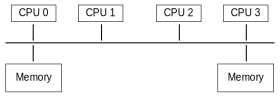
\includegraphics{memorder/SystemArchBus}}
\caption{Global System Bus And Multi-Copy Atomicity}
\label{fig:memorder:Global System Bus And Multi-Copy Atomicity}
\end{figure}

Threads running on a fully
\emph{multicopy atomic}~\cite{Stone:1995:SP:623262.623912}
platform are guaranteed
to agree on the order of stores, even to different variables.
A useful mental model of such a system is the single-bus architecture
shown in
\cref{fig:memorder:Global System Bus And Multi-Copy Atomicity}.
If each store resulted in a message on the bus, and if the bus could
accommodate only one store at a time, then any pair of CPUs would
agree on the order of all stores that they observed.
Unfortunately, building a computer system as shown in the figure,
without store buffers or even caches, would result in glacial computation.
Most CPU vendors interested in providing multicopy atomicity have therefore
instead provided the slightly weaker
\emph{other-multicopy atomicity}~\cite[Section B2.3]{ARMv8A:2017},
which excludes the CPU doing a given store from the requirement that all
CPUs agree on the order of all stores.\footnote{
	As of late 2018, ARMv8 and x86 provide other-multicopy atomicity,
	IBM mainframe provides fully multicopy atomicity, and PPC does
	not provide multicopy atomicity at all. More detail is shown in
	\cref{tab:memorder:Summary of Memory Ordering}.}
This means that if only a subset of CPUs are doing stores, the
other CPUs will agree on the order of stores, hence the ``other''
in ``other-multicopy atomicity''.
Unlike multicopy-atomic platforms, within other-multicopy-atomic platforms,
the CPU doing the store is permitted to observe its
store early, which allows its later loads to obtain the newly stored
value directly from the store buffer.
This in turn avoids abysmal performance.

\QuickQuiz{}
	Can you give a specific example showing different behavior for
	multicopy atomic on the one hand and other-multicopy atomic
	on the other?
\QuickQuizAnswer{
\begin{listing}[tbp]
\input{CodeSamples/formal/litmus/C-MP-OMCA+o-o-o+o-rmb-o@whole.fcv}
\caption{Litmus Test Distinguishing Multicopy Atomic From Other Multicopy Atomic}
\label{lst:memorder:Litmus Test Distinguishing Multicopy Atomic From Other Multicopy Atomic}
\end{listing}%
%
	\Cref{lst:memorder:Litmus Test Distinguishing Multicopy Atomic From Other Multicopy Atomic}
	(\path{C-MP-OMCA+o-o-o+o-rmb-o.litmus})
	shows such a test.

	\begin{lineref}[ln:formal:C-MP-OMCA+o-o-o+o-rmb-o:whole]
	On a multicopy-atomic platform, \co{P0()}'s store to \co{x} on
	\clnref{P0:st} must become visible to both \co{P0()} and \co{P1()}
	simultaneously.
	Because this store becomes visible to \co{P0()} on \clnref{P0:ld}, before
	\co{P0()}'s store to \co{y} on \clnref{P0:y}, \co{P0()}'s store to
	\co{x} must become visible before its store to \co{y} everywhere,
	including \co{P1()}.
	Therefore, if \co{P1()}'s load from \co{y} on \clnref{P1:y} returns the
	value 1, so must its load from \co{x} on \clnref{P1:x}, given that
	the \co{smp_rmb()} on \clnref{P1:rmb} forces these two loads to execute
	in order.
	Therefore, the \co{exists} clause on \clnref{exists} cannot trigger on a
	multicopy-atomic platform.
	\end{lineref}

	In contrast, on an other-multicopy-atomic platform, \co{P0()}
	could see its own store early, so that there would be no constraint
	on the order of visibility of the two stores from to \co{P1()},
	which in turn allows the \co{exists} clause to trigger.
} \QuickQuizEnd

Perhaps there will come a day when all platforms provide some flavor
of multi-copy atomicity, but
in the meantime, non-multicopy-atomic platforms do exist, and so software
must deal with them.

\begin{listing}[tbp]
\input{CodeSamples/formal/litmus/C-WRC+o+o-data-o+o-rmb-o@whole.fcv}
\caption{WRC Litmus Test With Dependencies (No Ordering)}
\label{lst:memorder:WRC Litmus Test With Dependencies (No Ordering)}
\end{listing}

\begin{lineref}[ln:formal:C-WRC+o+o-data-o+o-rmb-o:whole]
\Cref{lst:memorder:WRC Litmus Test With Dependencies (No Ordering)}
(\path{C-WRC+o+o-data-o+o-rmb-o.litmus})
demonstrates multicopy atomicity, that is, on a multicopy-atomic platform,
the \co{exists} clause on \clnref{exists} cannot trigger.
In contrast, on a non-multicopy-atomic
platform this \co{exists} clause can trigger, despite
\co{P1()}'s accesses being ordered by a data dependency and \co{P2()}'s
accesses being ordered by an \co{smp_rmb()}.
Recall that the definition of multicopy atomicity requires that all
threads agree on the order of stores, which can be thought of as
all stores reaching all threads at the same time.
Therefore, a non-multicopy-atomic platform can have a store reach
different threads at different times.
In particular, \co{P0()}'s store might reach \co{P1()} long before it
reaches \co{P2()}, which raises the possibility that \co{P1()}'s store
might reach \co{P2()} before \co{P0()}'s store does.
\end{lineref}

\begin{figure}[tb]
\centering
\resizebox{3.0in}{!}{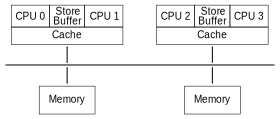
\includegraphics{memorder/NonMCAplatform}}
\caption{Shared Store Buffers And Multi-Copy Atomicity}
\label{fig:memorder:Shared Store Buffers And Multi-Copy Atomicity}
\end{figure}

This leads to the question of why a real system constrained by the
usual laws of physics would ever trigger the \co{exists} clause of
\cref{lst:memorder:WRC Litmus Test With Dependencies (No Ordering)}.
The cartoonish diagram of a such a real system is shown in
\cref{fig:memorder:Shared Store Buffers And Multi-Copy Atomicity}.
CPU~0 and CPU~1 share a store buffer, as do CPUs~2 and~3.
This means that CPU~1 can load a value out of the store buffer, thus
potentially immediately seeing a value stored by CPU~0.
In contrast, CPUs~2 and~3 will have to wait for the corresponding cache
line to carry this new value to them.

\QuickQuiz{}
	Then who would even \emph{think} of designing a system with shared
	store buffers???
\QuickQuizAnswer{
	This is in fact a very natural design for any system having
	multiple hardware threads per core.
	Natural from a hardware point of view, that is!
} \QuickQuizEnd

\begin{table*}[tbh]
\small
\centering\OneColumnHSpace{-0.8in}
\renewcommand*{\arraystretch}{1.1}
\rowcolors{10}{}{lightgray}
\begin{tabular}{rlllllll}\toprule
	& \multicolumn{1}{c}{\tco{P0()}} & \multicolumn{2}{c}{\tco{P0()} \& \tco{P1()}} &
		\multicolumn{1}{c}{\tco{P1()}} & \multicolumn{3}{c}{\tco{P2()}} \\
	\cmidrule(l){2-2} \cmidrule(l){3-4} \cmidrule(lr){5-5} \cmidrule(l){6-8}
	& Instruction & Store Buffer & Cache & Instruction &
			Instruction & Store Buffer & Cache \\
	\cmidrule{1-1} \cmidrule(l){2-2} \cmidrule(l){3-4}
		\cmidrule(lr){5-5} \cmidrule(l){6-8}
	1 & (Initial state) & & \tco{y==0} &
		(Initial state) &
			(Initial state) & & \tco{x==0} \\
	2 & \tco{x = 1;} & \tco{x==1} & \tco{y==0} &
		 & & & \tco{x==0} \\
	3 & (Read-Invalidate \tco{x}) & \tco{x==1} & \tco{y==0} & \tco{r1 = x} (1)
		 & & & \tco{x==0} \\
	4 &  & \tco{x==1} \tco{y==1} & \tco{y==0} & \tco{y = r1}
		 & \tco{r2 = y} & & \tco{x==0} \\
	5 &  & \tco{x==1} & \tco{y==1} & (Finish store)
		 & (Read \tco{y}) & & \tco{x==0} \\
	6 & (Respond \tco{y}) & \tco{x==1} & \tco{y==1} &
		 & (\tco{r2==1}) & & \tco{x==0} \tco{y==1} \\
	7 & & \tco{x==1} & \tco{y==1} &
		 & \tco{smp_rmb()} & & \tco{x==0} \tco{y==1} \\
	8 & & \tco{x==1} & \tco{y==1} &
		 & \tco{r3 = x (0)} & & \tco{x==0} \tco{y==1} \\
	9 & & \tco{x==1} & \tco{x==0} \tco{y==1} &
		 & (Respond \tco{x}) & & \tco{y==1} \\
	10 & (Finish store) & & \tco{x==1} \tco{y==1} &
		 &  & & \tco{y==1} \\
	\bottomrule
\end{tabular}
\caption{Memory Ordering: WRC Sequence of Events}
\label{tab:memorder:Memory Ordering: WRC Sequence of Events}
\end{table*}

\Cref{tab:memorder:Memory Ordering: WRC Sequence of Events}
shows one sequence of events that can result in the \co{exists} clause in
\cref{lst:memorder:WRC Litmus Test With Dependencies (No Ordering)}
triggering.
This sequence of events will depend critically on \co{P0()} and
\co{P1()} sharing both cache and a store buffer in the manner shown in
\cref{fig:memorder:Shared Store Buffers And Multi-Copy Atomicity}.

\QuickQuiz{}
	But just how is it fair that \co{P0()} and \co{P1()} must share a store
	buffer and a cache, but \co{P2()} gets one each of its very own???
\QuickQuizAnswer{
	Presumably there is a \co{P3()}, as is in fact shown in
	\cref{fig:memorder:Shared Store Buffers And Multi-Copy Atomicity},
	that shares \co{P2()}'s store buffer and cache.
	But not necessarily.
	Some platforms allow different cores to disable different numbers
	of threads, allowing the hardware to adjust to the needs of the
	workload at hand.
	For example, a single-threaded critical-path portion of the workload
	might be assigned to a core with only one thread enabled, thus
	allowing the single thread running that portion of the workload
	to use the entire capabilities of that core.
	Other more highly parallel but cache-miss-prone portions of the
	workload might be assigned to cores with all hardware threads
	enabled to provide improved throughput.
	This improved throughput could be due to the fact that while one
	hardware thread is stalled on a cache miss, the other hardware
	threads can make forward progress.

	In such cases, performance requirements override quaint human
	notions of fairness.
} \QuickQuizEnd

\begin{lineref}[ln:formal:C-WRC+o+o-data-o+o-rmb-o:whole]
Row~1 shows the initial state, with the initial value of \co{y} in
\co{P0()}'s and \co{P1()}'s shared cache, and the initial value of \co{x} in
\co{P2()}'s cache.

Row~2 shows the immediate effect of \co{P0()} executing its store on \clnref{P0:x}.
Because the cacheline containing \co{x} is not in \co{P0()}'s and \co{P1()}'s
shared cache, the new value (\co{1}) is stored in the shared store buffer.

Row~3 shows two transitions.
First, \co{P0()} issues a read-invalidate operation to fetch the cacheline
containing \co{x} so that it can flush the new value for \co{x} out of
the shared store buffer.
Second, \co{P1()} loads from \co{x} (\clnref{P1:x}), an operation that completes
immediately because the new value of \co{x} is immediately available
from the shared store buffer.

Row~4 also shows two transitions.
First, it shows the immediate effect of \co{P1()} executing its store to
\co{y} (\clnref{P1:y}), placing the new value into the shared store buffer.
Second, it shows the start of \co{P2()}'s load from \co{y} (\clnref{P2:y}).

Row~5 continues the tradition of showing two transitions.
First, it shows \co{P1()} complete its store to \co{y}, flushing
from the shared store buffer to the cache.
Second, it shows \co{P2()} request the cacheline containing \co{y}.

Row~6 shows \co{P2()} receive the cacheline containing \co{y}, allowing
it to finish its load into \co{r2}, which takes on the value \co{1}.

Row~7 shows \co{P2()} execute its \co{smp_rmb()} (\clnref{P2:rmb}), thus keeping
its two loads ordered.

Row~8 shows \co{P2()} execute its load from \co{x}, which immediately
returns with the value zero from \co{P2()}'s cache.

Row~9 shows \co{P2()} \emph{finally} responding to \co{P0()}'s request for
the cacheline containing \co{x}, which was made way back up on row~3.

Finally, row~10 shows \co{P0()} finish its store, flushing its value of
\co{x} from the shared store buffer to the shared cache.

Note well that the \co{exists} clause on \clnref{exists} has triggered.
The values of \co{r1} and \co{r2} are both the value one, and
the final value of \co{r3} the value zero.
This strange result occurred because \co{P0()}'s new value of \co{x} was
communicated to \co{P1()} long before it was communicated to \co{P2()}.
\end{lineref}

\QuickQuiz{}
	\begin{lineref}[ln:formal:C-WRC+o+o-data-o+o-rmb-o:whole]
	Referring to
	\cref{tab:memorder:Memory Ordering: WRC Sequence of Events},
	why on earth would \co{P0()}'s store take so long to complete when
	\co{P1()}'s store complete so quickly?
	In other words, does the \co{exists} clause on \clnref{exists} of
	\cref{lst:memorder:WRC Litmus Test With Dependencies (No Ordering)}
	really trigger on real systems?
	\end{lineref}
\QuickQuizAnswer{
	You need to face the fact that it really can trigger.
	Akira Yokosawa used the \co{litmus7} tool to run this litmus test
	on a \Power{8} system.
	Out of 1,000,000,000 runs, 4 triggered the \co{exists} clause.
	Thus, triggering the \co{exists} clause is not merely a one-in-a-million
	occurrence, but rather a one-in-a-hundred-million occurrence.
	But it nevertheless really does trigger on real systems.
} \QuickQuizEnd

This counter-intuitive result happens because although dependencies
do provide ordering, they provide it only within the confines of their
own thread.
This three-thread example requires stronger ordering, which
is the subject of
\crefthro{sec:memorder:Cumulativity}
{sec:memorder:Release-Acquire Chains}.

\subsubsection{Cumulativity}
\label{sec:memorder:Cumulativity}

The three-thread example shown in
\cref{lst:memorder:WRC Litmus Test With Dependencies (No Ordering)}
requires \emph{cumulative} ordering, or \emph{cumulativity}.
A cumulative memory-ordering operation orders not just any given
access preceding it, but also earlier accesses by any thread to that
same variable.

\begin{listing}[tbp]
\input{CodeSamples/formal/litmus/C-WRC+o+o-r+a-o@whole.fcv}
\caption{WRC Litmus Test With Release}
\label{lst:memorder:WRC Litmus Test With Release}
\end{listing}

Dependencies do not provide cumulativity,
which is why the ``C'' column is blank for
both the \co{READ_ONCE()} and the \co{smp_read_barrier_depends()} rows
of \cref{tab:memorder:Linux-Kernel Memory-Ordering Cheat Sheet}.
However, as indicated by the ``C'' in their ``C'' column,
release operations do provide cumulativity.
Therefore,
\cref{lst:memorder:WRC Litmus Test With Release}
(\path{C-WRC+o+o-r+a-o.litmus})
substitutes a release operation for
\cref{lst:memorder:WRC Litmus Test With Dependencies (No Ordering)}'s
data dependency.
\begin{lineref}[ln:formal:C-WRC+o+o-r+a-o:whole]
Because the release operation is cumulative, its ordering applies not only to
\cref{lst:memorder:WRC Litmus Test With Release}'s
load from \co{x} by \co{P1()} on \clnref{P1:x}, but also to the store to \co{x}
by \co{P0()} on \clnref{P0:x}---but only if that load returns the value stored,
which matches the \co{1:r1=1} in the \co{exists} clause on \clnref{exists}.
This means that \co{P2()}'s load-acquire suffices to force the
load from \co{x} on \clnref{P2:x} to happen after the store on \clnref{P0:x}, so
the value returned is one, which does not match \co{2:r3=0}, which
in turn prevents the \co{exists} clause from triggering.
\end{lineref}

\begin{figure*}[htbp]
\centering
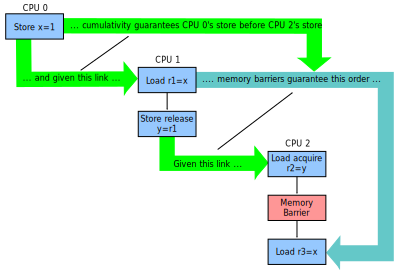
\includegraphics{memorder/memorybarriercum}
\caption{Cumulativity}
\label{fig:memorder:Cumulativity}
\end{figure*}

\begin{lineref}[ln:formal:C-WRC+o+o-r+a-o:whole]
These ordering constraints are depicted graphically in
\cref{fig:memorder:Cumulativity}.
Note also that cumulativity is not limited to a single step back in time.
If there was another load from \co{x} or store to \co{x} from any thread
that came before the store on \clnref{P0:x}, that prior load or store would also
be ordered before the load on \clnref{P2:x}, though only if both \co{r1} and
\co{r2} both end up containing the value \co{1}.
\end{lineref}

In short, use of cumulative ordering operations can suppress
non-multicopy-atomic behaviors in some situations.
Cumulativity nevertheless has limits, which are examined in the next section.

\subsubsection{Propagation}
\label{sec:memorder:Propagation}

\begin{listing}[tbp]
\input{CodeSamples/formal/litmus/C-W+RWC+o-r+a-o+o-mb-o@whole.fcv}
\caption{W+RWC Litmus Test With Release (No Ordering)}
\label{lst:memorder:W+RWC Litmus Test With Release (No Ordering)}
\end{listing}

\begin{lineref}[ln:formal:C-W+RWC+o-r+a-o+o-mb-o:whole]
\Cref{lst:memorder:W+RWC Litmus Test With Release (No Ordering)}
(\path{C-W+RWC+o-r+a-o+o-mb-o.litmus})
shows the limitations of cumulativity and store-release,
even with a full memory barrier.
The problem is that although the \co{smp_store_release()} on
\clnref{P0:sr} has cumulativity, and although that cumulativity does
order \co{P2()}'s load on \clnref{P2:ld}, the \co{smp_store_release()}'s
ordering cannot propagate through the combination of \co{P1()}'s
load (\clnref{P1:ld}) and \co{P2()}'s store (\clnref{P2:st}).
This means that the \co{exists} clause on \clnref{exists} really can trigger.
\end{lineref}

\QuickQuiz{}
	But it is not necessary to worry about propagation unless
	there are at least three threads in the litmus test, right?
\QuickQuizAnswer{
\begin{listing}[tbp]
\input{CodeSamples/formal/litmus/C-R+o-wmb-o+o-mb-o@whole.fcv}
\caption{R Litmus Test With Write Memory Barrier (No Ordering)}
\label{lst:memorder:R Litmus Test With Write Memory Barrier (No Ordering)}
\end{listing}%
%
	Wrong.

	\begin{lineref}[ln:formal:C-R+o-wmb-o+o-mb-o:whole]
	\Cref{lst:memorder:R Litmus Test With Write Memory Barrier (No Ordering)}
	(\path{C-R+o-wmb-o+o-mb-o.litmus})
	shows a two-thread litmus test that requires propagation due to
	the fact that it only has store-to-store and load-to-store
	links between its pair of threads.
	Even though \co{P0()} is fully ordered by the \co{smp_wmb()} and
	\co{P1()} is fully ordered by the \co{smp_mb()}, the
	counter-temporal nature of the links means that
	the \co{exists} clause on \clnref{exists} really can trigger.
	To prevent this triggering, the \co{smp_wmb()} on \clnref{wmb}
	must become an \co{smp_mb()}, bringing propagation into play
	twice, once for each non-temporal link.
	\end{lineref}
} \QuickQuizEnd

\QuickQuizLabel{\MemorderQQLitmusTestR}

\begin{figure}[htbp]
\centering
\resizebox{\twocolumnwidth}{!}{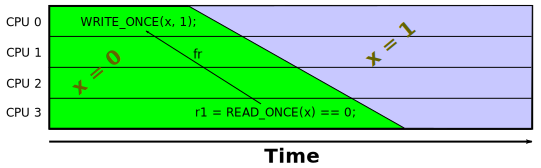
\includegraphics{memorder/fr}}
\caption{Load-to-Store is Counter-Temporal}
\label{fig:memorder:Load-to-Store is Counter-Temporal}
\end{figure}

This situation might seem completely counter-intuitive, but keep
in mind that the speed of light is finite and computers are of
non-zero size.
It therefore takes time for the effect of the \co{P2()}'s store to
\co{z} to propagate to \co{P1()}, which in turn means that it is possible
that \co{P1()}'s read from \co{z} happens much later in time, but
nevertheless still sees the old value of zero.
This situation is depicted in
\cref{fig:memorder:Load-to-Store is Counter-Temporal}:
Just because a load sees the old value does \emph{not} mean that
this load executed at an earlier time than did the store of the
new value.

Note that
\cref{lst:memorder:W+RWC Litmus Test With Release (No Ordering)}
also shows the limitations of memory-barrier pairing, given that
there are not two but three processes.
These more complex litmus tests can instead be said to have \emph{cycles},
where memory-barrier pairing is the special case of a two-thread cycle.
\begin{lineref}[ln:formal:C-W+RWC+o-r+a-o+o-mb-o:whole]
The cycle in
\cref{lst:memorder:W+RWC Litmus Test With Release (No Ordering)}
goes through \co{P0()} (\clnref{P0:st,P0:sr}), \co{P1()} (\clnref{P1:la,P1:ld}),
\co{P2()} (\clnref{P2:st,P2:mb,P2:ld}), and back to \co{P0()} (\clnref{P0:st}).
The \co{exists} clause delineates this cycle:
the \co{1:r1=1} indicates that the \co{smp_load_acquire()} on \clnref{P1:la}
returned the value stored by the \co{smp_store_release()} on \clnref{P0:sr},
the \co{1:r2=0} indicates that the \co{WRITE_ONCE()} on \clnref{P2:st} came
too late to affect the value returned by the \co{READ_ONCE()} on \clnref{P1:ld},
and finally the \co{2:r3=0} indicates that the
\co{WRITE_ONCE()} on \clnref{P0:st} came too late to affect the value returned
by the \co{READ_ONCE()} on \clnref{P2:ld}.
In this case, the fact that the \co{exists} clause can trigger means that
the cycle is said to be \emph{allowed}.
In contrast, in cases where the \co{exists} clause cannot trigger,
the cycle is said to be \emph{prohibited}.
\end{lineref}

\begin{listing}[tbp]
\input{CodeSamples/formal/litmus/C-W+RWC+o-mb-o+a-o+o-mb-o@whole.fcv}
\caption{W+WRC Litmus Test With More Barriers}
\label{lst:memorder:W+WRC Litmus Test With More Barriers}
\end{listing}

\begin{lineref}[ln:formal:C-W+RWC+o-r+a-o+o-mb-o:whole]
But what if we need to keep the \co{exists} clause on \clnref{exists} of
\cref{lst:memorder:W+RWC Litmus Test With Release (No Ordering)}?
One solution is to replace \co{P0()}'s \co{smp_store_release()}
with an \co{smp_mb()}, which
\cref{tab:memorder:Linux-Kernel Memory-Ordering Cheat Sheet}
shows to have not only cumulativity, but also propagation.
\end{lineref}
The result is shown in
\cref{lst:memorder:W+WRC Litmus Test With More Barriers}
(\path{C-W+RWC+o-mb-o+a-o+o-mb-o.litmus}).

\QuickQuiz{}
	\begin{lineref}[ln:formal:C-W+RWC+o-r+a-o+o-mb-o:whole]
	But given that \co{smp_mb()} has the propagation property,
	why doesn't the \co{smp_mb()} on \clnref{P2:mb} of
	\cref{lst:memorder:W+RWC Litmus Test With Release (No Ordering)}
	prevent the \co{exists} clause from triggering?
	\end{lineref}
\QuickQuizAnswer{
	\begin{lineref}[ln:formal:C-W+RWC+o-r+a-o+o-mb-o:whole]
	As a rough rule of thumb, the \co{smp_mb()} barrier's
	propagation property is sufficient to maintain ordering
	through only one load-to-store link between
	processes.
	Unfortunately,
	\cref{lst:memorder:W+RWC Litmus Test With Release (No Ordering)}
	has not one but two load-to-store links, with the
	first being from the \co{READ_ONCE()} on \clnref{P1:ld} to the
	\co{WRITE_ONCE()} on \clnref{P2:st} and the second being from
	the \co{READ_ONCE()} on \clnref{P2:ld} to the \co{WRITE_ONCE()}
	on \clnref{P0:st}.
	Therefore, preventing the \co{exists} clause from triggering
	should be expected to require not one but two
	instances of \co{smp_mb()}.
	\end{lineref}

	As a special exception to this rule of thumb, a release-acquire
	chain can have one load-to-store link between processes
	and still prohibit the cycle.
} \QuickQuizEnd

\begin{figure}[tbp]
\centering
\resizebox{\twocolumnwidth}{!}{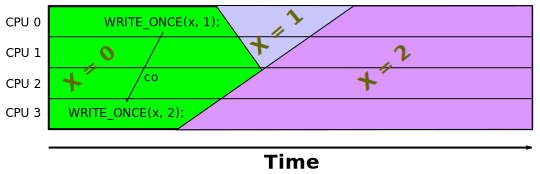
\includegraphics{memorder/co}}
\caption{Store-to-Store is Counter-Temporal}
\label{fig:memorder:Store-to-Store is Counter-Temporal}
\end{figure}

For completeness,
\cref{fig:memorder:Store-to-Store is Counter-Temporal}
shows that the ``winning'' store among a group of stores to the
same variable is not necessarily the store that started last.
This should not come as a surprise to anyone who carefully examined
\cref{fig:memorder:A Variable With More Simultaneous Values}.

\begin{listing}[tbp]
\input{CodeSamples/formal/litmus/C-2+2W+o-wmb-o+o-wmb-o@whole.fcv}
\caption{2+2W Litmus Test With Write Barriers}
\label{lst:memorder:2+2W Litmus Test With Write Barriers}
\end{listing}

\QuickQuiz{}
	But for litmus tests having only ordered stores, as shown in
	\cref{lst:memorder:2+2W Litmus Test With Write Barriers}
	(\path{C-2+2W+o-wmb-o+o-wmb-o.litmus}),
	research shows that the cycle is prohibited, even in weakly
	ordered systems such as ARM and Power~\cite{test6-pdf}.
	Given that, are store-to-store really \emph{always}
	counter-temporal???
\QuickQuizAnswer{
	This litmus test is indeed a very interesting curiosity.
	Its ordering apparently occurs naturally given typical
	weakly ordered hardware design, which would normally be
	considered a great gift from the relevant laws of physics
	and cache-coherency-protocol mathematics.

	\begin{lineref}[ln:formal:C-2+2W+o-wmb-o+o-wmb-o:whole]
	Unfortunately, no one has been able to come up with a software use
	case for this gift that does not have a much better alternative
	implementation.
	Therefore, neither the C11 nor the Linux kernel memory models
	provide any guarantee corresponding to
	\cref{lst:memorder:2+2W Litmus Test With Write Barriers}.
	This means that the \co{exists} clause on \clnref{exists} can
	trigger.
	\end{lineref}

\begin{listing}[tbp]
\input{CodeSamples/formal/litmus/C-2+2W+o-o+o-o@whole.fcv}
\caption{2+2W Litmus Test (No Ordering)}
\label{lst:memorder:2+2W Litmus Test (No Ordering)}
\end{listing}

	Of course, without the barrier, there are no ordering
	guarantees, even on real weakly ordered hardware, as shown in
	\cref{lst:memorder:2+2W Litmus Test (No Ordering)}
	(\path{C-2+2W+o-o+o-o.litmus}).
} \QuickQuizEnd

But sometimes time really is on our side.  Read on!

\subsubsection{Happens-Before}
\label{sec:memorder:Happens-Before}

\begin{figure}[tbp]
\centering
\resizebox{\twocolumnwidth}{!}{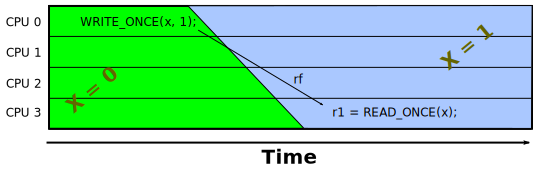
\includegraphics{memorder/rf}}
\caption{Store-to-Load is Temporal}
\label{fig:memorder:Store-to-Load is Temporal}
\end{figure}

As shown in
\cref{fig:memorder:Store-to-Load is Temporal},
on platforms without user-visible speculation, if a load returns the value
from a particular store, then, courtesy of the finite speed of light and
the non-zero size of modern computing systems, the store absolutely has
to have executed at an earlier time than did the load.
This means that carefully constructed programs can rely on the
passage of time itself as an memory-ordering operation.

\begin{listing}[tbp]
\input{CodeSamples/formal/litmus/C-LB+a-o+o-data-o+o-data-o@whole.fcv}
\caption{LB Litmus Test With One Acquire}
\label{lst:memorder:LB Litmus Test With One Acquire}
\end{listing}

Of course, just the passage of time by itself is not enough, as
was seen in
\cref{lst:memorder:Load-Buffering Litmus Test (No Ordering)},
which has nothing but store-to-load links and, because it provides
absolutely no ordering, still can trigger its \co{exists} clause.
However, as long as each thread provides even the weakest possible
ordering, \co{exists} clause would not be able to trigger.
For example,
\cref{lst:memorder:LB Litmus Test With One Acquire}
(\path{C-LB+a-o+o-data-o+o-data-o.litmus})
shows \co{P0()} ordered with an \co{smp_load_acquire()} and
both \co{P1()} and \co{P2()} ordered with data dependencies.
These orderings, which are close to the top of
\cref{tab:memorder:Linux-Kernel Memory-Ordering Cheat Sheet},
suffice to prevent the \co{exists} clause from triggering.

\QuickQuiz{}
	Can you construct a litmus test like that in
	\cref{lst:memorder:LB Litmus Test With One Acquire}
	that uses \emph{only} dependencies?
\QuickQuizAnswer{
	\Cref{lst:memorder:LB Litmus Test With No Acquires}
	shows a somewhat nonsensical but very real example.
	Creating a more useful (but still real) litmus test is left
	as an exercise for the reader.

\begin{listing}[tbp]
\input{CodeSamples/formal/litmus/C-LB+o-data-o+o-data-o+o-data-o@whole.fcv}
\caption{LB Litmus Test With No Acquires}
\label{lst:memorder:LB Litmus Test With No Acquires}
\end{listing}
} \QuickQuizEnd

An important, to say nothing of more useful, use of time for ordering
memory accesses is covered in the next section.

\subsubsection{Release-Acquire Chains}
\label{sec:memorder:Release-Acquire Chains}

\begin{listing}[tbp]
\input{CodeSamples/formal/litmus/C-LB+a-r+a-r+a-r+a-r@whole.fcv}
\caption{Long LB Release-Acquire Chain}
\label{lst:memorder:Long LB Release-Acquire Chain}
\end{listing}

A minimal release-acquire chain was shown in
\cref{lst:memorder:Enforcing Ordering of Load-Buffering Litmus Test},
but these chains can be much longer, as shown in
\cref{lst:memorder:Long LB Release-Acquire Chain}
(\path{C-LB+a-r+a-r+a-r+a-r.litmus}).
The longer the release-acquire chain, the more ordering is gained
from the passage of time, so that no matter how many threads are
involved, the corresponding \co{exists} clause cannot trigger.

\begin{listing}[tbp]
\input{CodeSamples/formal/litmus/C-ISA2+o-r+a-r+a-r+a-o@whole.fcv}
\caption{Long ISA2 Release-Acquire Chain}
\label{lst:memorder:Long ISA2 Release-Acquire Chain}
\end{listing}

Although release-acquire chains are inherently store-to-load creatures,
it turns out that they can tolerate one load-to-store step, despite
such steps being counter-temporal, as shown in
\cref{fig:memorder:Load-to-Store is Counter-Temporal}.
For example,
\cref{lst:memorder:Long ISA2 Release-Acquire Chain}
(\path{C-ISA2+o-r+a-r+a-r+a-o.litmus})
shows a three-step release-acquire chain, but where \co{P3()}'s
final access is a \co{READ_ONCE()} from \co{x0}, which is
accessed via \co{WRITE_ONCE()} by \co{P0()}, forming a non-temporal
load-to-store link between these two processes.
\begin{lineref}[ln:formal:litmus:C-ISA2+o-r+a-r+a-r+a-o:whole]
However, because \co{P0()}'s \co{smp_store_release()} (\clnref{P0:rel})
is cumulative, if \co{P3()}'s \co{READ_ONCE()} returns zero,
this cumulativity will force the \co{READ_ONCE()} to be ordered
before \co{P0()}'s \co{smp_store_release()}.
In addition, the release-acquire chain
(\clnref{P0:rel,P1:acq,P1:rel,P2:acq,P2:rel,P3:acq})
forces \co{P3()}'s \co{READ_ONCE()} to be ordered after \co{P0()}'s
\co{smp_store_release()}.
Because \co{P3()}'s \co{READ_ONCE()} cannot be both before and after
\co{P0()}'s \co{smp_store_release()}, either or both of two things must
be true:
\end{lineref}

\begin{enumerate}
\item	\co{P3()}'s \co{READ_ONCE()} came after \co{P0()}'s
	\co{WRITE_ONCE()}, so that the \co{READ_ONCE()} returned
	the value two, so that the \co{exists} clause's \co{3:r2=0}
	is false.
\item	The release-acquire chain did not form, that is, one or more
	of the \co{exists} clause's \co{1:r2=2}, \co{2:r2=2}, or \co{3:r1=2}
	is false.
\end{enumerate}

Either way, the \co{exists} clause cannot trigger, despite this litmus
test containing a notorious load-to-store link between
\co{P3()} and \co{P0()}.
But never forget that release-acquire chains can tolerate only one
load-to-store link, as was seen in
\cref{lst:memorder:W+RWC Litmus Test With Release (No Ordering)}.

\begin{listing}[tbp]
\input{CodeSamples/formal/litmus/C-Z6.2+o-r+a-r+a-r+a-o@whole.fcv}
\caption{Long Z6.2 Release-Acquire Chain}
\label{lst:memorder:Long Z6.2 Release-Acquire Chain}
\end{listing}

Release-acquire chains can also tolerate a single store-to-store step,
as shown in
\cref{lst:memorder:Long Z6.2 Release-Acquire Chain}
(\path{C-Z6.2+o-r+a-r+a-r+a-o.litmus}).
\begin{lineref}[ln:formal:C-Z6.2+o-r+a-r+a-r+a-o:whole]
As with the previous example, \co{smp_store_release()}'s cumulativity
combined with the temporal nature of the release-acquire chain
prevents the \co{exists} clause on \clnref{exists} from triggering.
But beware: Adding a second store-to-store step would allow the correspondingly
updated \co{exists} clause to trigger.
\end{lineref}

\begin{listing}[tbp]
\input{CodeSamples/formal/litmus/C-Z6.2+o-r+a-o+o-mb-o@whole.fcv}
\caption{Z6.0 Release-Acquire Chain (Ordering?)}
\label{lst:memorder:Z6.0 Release-Acquire Chain (Ordering?)}
\end{listing}

\QuickQuiz{}
	Suppose we have a short release-acquire chain along with one
	load-to-store link and one store-to-store link, like that shown in
	\cref{lst:memorder:Z6.0 Release-Acquire Chain (Ordering?)}.
	Given that there is only one of each type of non-store-to-load
	link, the \co{exists} cannot trigger, right?
\QuickQuizAnswer{
	Wrong.
	It is the number of non-store-to-load links that matters.
	If there is only one non-store-to-load link, a release-acquire
	chain can prevent the \co{exists} clause from triggering.
	However, if there is more than one non-store-to-load link,
	be they store-to-store, load-to-store, or any combination
	thereof, it is necessary to have at least one full barrier
	(\co{smp_mb()} or better) between each non-store-to-load link.
	In
	\cref{lst:memorder:Z6.0 Release-Acquire Chain (Ordering?)},
	preventing the \co{exists} clause from triggering therefore requires
	an additional full barrier between either \co{P0()}'s or
	\co{P1()}'s accesses.
} \QuickQuizEnd

\QuickQuiz{}
	There are store-to-load links, load-to-store links, and
	store-to-store links.
	But what about load-to-load links?
\QuickQuizAnswer{
	The problem with the concept of load-to-load links is that
	if the two loads from the same variable return the same
	value, there is no way to determine their ordering.
	The only way to determine their ordering is if they return
	different values, in which case there had to have been an
	intervening store.
	And that intervening store means that there is no load-to-load
	link, but rather a load-to-store link followed by a
	store-to-load link.
} \QuickQuizEnd

In short, properly constructed release-acquire chains form a peaceful
island of intuitive bliss surrounded by a strongly counter-intuitive
sea of more complex memory-ordering constraints.

% Exercises?
% Hardware details from Appendix?

\section{Compile-Time Consternation}
\label{sec:memorder:Compile-Time Consternation}

Most languages, including C, were developed on uniprocessor systems
by people with little or no parallel-programming experience.
As a results, unless explicitly told otherwise, these languages assume
that the current CPU is the only thing that is reading or writing memory.
This in turn means that these languages' compilers' optimizers
are ready, willing, and oh so able to make dramatic changes to the
order, number, and sizes of memory references that your program
executes.
In fact, the reordering carried out by hardware can seem quite tame
by comparison.

This section will help you tame your compiler, thus avoiding a great
deal of compile-time consternation.
\Cref{sec:memorder:Memory-Reference Restrictions}
describes how to keep the compiler from destructively optimizing
your code's memory references,
\cref{sec:memorder:Address- and Data-Dependency Difficulties}
describes how to protect address and data dependencies,
and finally,
\cref{sec:memorder:Control-Dependency Calamities}
describes how to protect those delicate control dependencies.

\subsection{Memory-Reference Restrictions}
\label{sec:memorder:Memory-Reference Restrictions}

As noted in \cref{sec:toolsoftrade:Accessing Shared Variables},
unless told otherwise, compilers assume that nothing else
is affecting the variables that the code is accessing.
Furthermore, this assumption is not simply some design error, but is
instead enshrined in various standards.\footnote{
	Or perhaps it is a standardized design error.}
It is worth summarizing this material in preparation for the following
sections.

Plain accesses, as in plain-access C-language assignment statements such
as \qco{r1 = a} or \qco{b = 1} are subject to the
shared-variable shenanigans described in
\cref{sec:toolsoftrade:Shared-Variable Shenanigans}.
Ways of avoiding these shenanigans are described in
\crefrange{sec:toolsoftrade:A Volatile Solution}{sec:toolsoftrade:Avoiding Data Races}:

\begin{enumerate}
\item	Plain accesses can tear, for example, the compiler could choose
	to access an eight-byte pointer one byte at a time.
	Tearing can be prevented by using \co{READ_ONCE()} and
	\co{WRITE_ONCE()}.
\item	Plain loads can fuse, for example, if the results of an earlier
	load from that same object are still in a machine register,
	the compiler might opt to reuse the value in that register
	instead of reloading from memory.
	Load fusing can be prevented by using \co{READ_ONCE()} or by
	enforcing ordering between the two loads using \co{barrier()},
	\co{smp_rmb()}, and other means shown in
	\cref{tab:memorder:Linux-Kernel Memory-Ordering Cheat Sheet}.
\item	Plain stores can fuse, so that a store can be omitted entirely
	if there is a later store to that same variable.
	Store fusing can be prevented by using \co{WRITE_ONCE()} or by
	enforcing ordering between the two stores using \co{barrier()},
	\co{smp_wmb()}, and other means shown in
	\cref{tab:memorder:Linux-Kernel Memory-Ordering Cheat Sheet}.
\item	Plain accesses can be reordered in surprising ways by modern
	optimizing compilers.
	This reordering can be prevented by enforcing ordering as
	called out above.
\item	Plain loads can be invented, for example, register pressure might
	cause the compiler to discard a previously loaded value from
	its register, and then reload it later on.
	Invented loads can be prevented by using \co{READ_ONCE()} or by
	enforcing ordering as called out above between the load and a
	later use of its value using \co{barrier()}.
\item	Stores can be invented before a plain store, for example, by
	using the stored-to location as temporary storage.
	This can be prevented by use of \co{WRITE_ONCE()}.
\end{enumerate}

\QuickQuiz{}
	Why not place a \co{barrier()} call immediately before
	a plain store to prevent the compiler from inventing stores?
\QuickQuizAnswer{
	Because it would not work.
	Although the compiler would be prevented from inventing a
	store prior to the \co{barrier()}, nothing would prevent
	it from inventing a store between that \co{barrier()} and
	the plain store.
} \QuickQuizEnd

Please note that all of these shared-memory shenanigans can instead be
avoided by avoiding data races on plain accesses, as described in
\cref{sec:toolsoftrade:Avoiding Data Races}.
After all, if there are no data races, then each and every one of the
compiler optimizations mentioned above is perfectly safe.
But for code containing data races, this list is subject to change
without notice as compiler optimizations continue becoming increasingly
aggressive.

In short, use of \co{READ_ONCE()}, \co{WRITE_ONCE()}, \co{barrier()},
\co{volatile}, and other primitives called out in
\cref{tab:memorder:Linux-Kernel Memory-Ordering Cheat Sheet}
are valuable tools in preventing the compiler from
optimizing your parallel algorithm out of existence.
Compilers are starting to provide other mechanisms for avoiding
load and store tearing, for example, \co{memory_order_relaxed}
atomic loads and stores, however, work is still
needed~\cite{JonathanCorbet2016C11atomics}.
In addition, compiler issues aside, \co{volatile} is still needed
to avoid fusing and invention of accesses, including C11 atomic accesses.

Please note that, it is possible to overdo use of \co{READ_ONCE()} and
\co{WRITE_ONCE()}.
For example, if you have prevented a given variable from changing
(perhaps by holding the lock guarding all updates to that
variable), there is no point in using \co{READ_ONCE()}.
Similarly, if you have prevented any other CPUs or threads from
reading a given variable (perhaps because you are initializing
that variable before any other CPU or thread has access to it),
there is no point in using \co{WRITE_ONCE()}.
However, in my experience, developers need to use things like
\co{READ_ONCE()} and \co{WRITE_ONCE()} more often than they think that
they do, the overhead of unnecessary uses is quite low.
Furthermore, the penalty for failing to use them when needed is quite high.

\subsection{Address- and Data-Dependency Difficulties}
\label{sec:memorder:Address- and Data-Dependency Difficulties}
\OriginallyPublished{Section}{sec:memorder:Address- and Data-Dependency Difficulties}{Address- and Data-Dependency Difficulties}{the Linux kernel}{PaulEMcKenney2014rcu-dereference}

Compilers do not understand either address or data dependencies,
although there are efforts underway to teach them, or at the very
least, standardize the process of teaching
them~\cite{PaulEMcKennneyConsumeP0190R4,PaulEMcKenney2017markconsumeP0462R1}.
In the meantime, it is necessary to be very careful in order to prevent
your compiler from breaking your dependencies.

\subsubsection{Give your dependency chain a good start}
The load that heads your dependency chain must use proper
ordering, for example \co{rcu_dereference()} or \co{READ_ONCE()}.
Failure to follow this rule can have serious side effects:

\begin{enumerate}
\item	On DEC Alpha, a dependent load might not be ordered with
	the load heading the dependency chain, as described in
	\cref{sec:memorder:Alpha}.
\item	If the load heading the dependency chain is a
	C11 non-volatile \co{memory_order_relaxed} load,
	the compiler could omit the load, for example, by using a value
	that it loaded in the past.
\item	If the load heading the dependency chain is a plain load,
	the compiler can omit the load, again by using a value
	that it loaded in the past.
	Worse yet, it could load twice instead of once, so that
	different parts of your code use different values---and
	compilers really do this, especially when under register
	pressure.
\item	The value loaded by the head of the dependency chain must
	be a pointer.
	In theory, yes, you could load an integer, perhaps to use
	it as an array index.
	In practice, the compiler knows too much about integers,
	and thus has way too many opportunities to break your
	dependency chain~\cite{PaulEMcKennneyConsumeP0190R4}.
\end{enumerate}

\subsubsection{Avoid arithmetic dependency breakage}
Although it is just fine to do some arithmetic operations on a pointer in
your dependency chain, you need to be careful to avoid giving the
compiler too much information.
After all, if the compiler learns enough to determine the exact value
of the pointer, it can use that exact value instead of the pointer itself.
As soon as the compiler does that, the dependency is broken and all
ordering is lost.

\begin{listing}[tbp]
\begin{linelabel}[ln:memorder:Breakable Dependencies With Comparisons]
\begin{VerbatimL}[commandchars=\\\[\]]
int reserve_int;
int *gp;
int *p;

p = rcu_dereference(gp);
if (p == &reserve_int)		\lnlbl[cmp]
	handle_reserve(p);	\lnlbl[handle]
do_something_with(*p); /* buggy! */
\end{VerbatimL}
\end{linelabel}
\caption{Breakable Dependencies With Comparisons}
\label{lst:memorder:Breakable Dependencies With Comparisons}
\end{listing}

\begin{listing}[tbp]
\begin{linelabel}[ln:memorder:Broken Dependencies With Comparisons]
\begin{VerbatimL}[commandchars=\\\[\]]
int reserve_int;
int *gp;
int *p;

p = rcu_dereference(gp);	\lnlbl[deref1]
if (p == &reserve_int) {
	handle_reserve(&reserve_int);
	do_something_with(reserve_int); /* buggy! */ \lnlbl[deref2]
} else {
	do_something_with(*p); /* OK! */
}
\end{VerbatimL}
\end{linelabel}
\caption{Broken Dependencies With Comparisons}
\label{lst:memorder:Broken Dependencies With Comparisons}
\end{listing}

\begin{enumerate}
\item	Although it is permissible to compute offsets from a
	pointer, these offsets must not result in total cancellation.
	For example, given a \co{char} pointer \co{cp},
	\co{cp-(uintptr_t)cp)} will cancel and can allow the compiler
	to break your dependency chain.
	On the other hand, canceling offset values with each other
	is perfectly safe and legal.
	For example, if \co{a} and \co{b} are equal, \co{cp+a-b}
	is an identity function, including preserving the dependency.
\item	Comparisons can break dependencies.
	\cref{lst:memorder:Breakable Dependencies With Comparisons}
	shows how this can happen.
	Here global pointer \co{gp} points to a dynamically allocated
	integer, but if memory is low, it might instead point to
	the \co{reserve_int} variable.
	\begin{lineref}[ln:memorder:Breakable Dependencies With Comparisons]
	This \co{reserve_int} case might need special handling, as
	shown on \clnref{cmp,handle} of the listing.
	\end{lineref}
        \begin{lineref}[ln:memorder:Broken Dependencies With Comparisons]
	But the compiler could reasonably transform this code into
	the form shown in
	\cref{lst:memorder:Broken Dependencies With Comparisons},
	especially on systems where instructions with absolute
	addresses run faster than instructions using addresses
	supplied in registers.
	However, there is clearly no ordering between the pointer
	load on \clnref{deref1} and the dereference on \clnref{deref2}.
	Please note that this is simply an example: There are a great
	many other ways to break dependency chains with comparisons.
	\end{lineref}
\end{enumerate}

\QuickQuiz{}
	\begin{lineref}[ln:memorder:Breakable Dependencies With Comparisons]
	Why can't you simply dereference the pointer before comparing it
	to \co{&reserve_int} on \clnref{cmp} of
	\cref{lst:memorder:Breakable Dependencies With Comparisons}?
	\end{lineref}
\QuickQuizAnswer{
	For first, it might be necessary to invoke
	\co{handle_reserve()} before \co{do_something_with()}.

	But more relevant to memory ordering, the compiler is often within
	its rights to hoist the comparison ahead of the dereferences,
	which would allow the compiler to use \co{&reserve_int} instead
	of the variable \co{p} that the hardware has tagged with
	a dependency.
} \QuickQuizEnd

\QuickQuiz{}
	But it should be safe to compare two pointer variables,
	right?  After all, the compiler doesn't know the value
	of either, so how can it possibly learn anything from the
	comparison?
\QuickQuizAnswer{
%
\begin{listing}[tbp]
\begin{linelabel}[ln:memorder:Breakable Dependencies With Non-Constant Comparisons]
\begin{VerbatimL}
int *gp1;
int *gp2;
int *p;
int *q;

p = rcu_dereference(gp1);
q = READ_ONCE(gp2);
if (p == q)
	handle_equality(p);
do_something_with(*p);
\end{VerbatimL}
\end{linelabel}
\caption{Breakable Dependencies With Non-Constant Comparisons}
\label{lst:memorder:Breakable Dependencies With Non-Constant Comparisons}
\end{listing}%
%
\begin{listing}[tbp]
\begin{linelabel}[ln:memorder:Broken Dependencies With Non-Constant Comparisons]
\begin{VerbatimL}[commandchars=\\\[\]]
int *gp1;
int *gp2;
int *p;
int *q;

p = rcu_dereference(gp1);		\lnlbl[p]
q = READ_ONCE(gp2);
if (p == q) {
	handle_equality(q);
	do_something_with(*q);		\lnlbl[q]
} else {
	do_something_with(*p);
}
\end{VerbatimL}
\end{linelabel}
\caption{Broken Dependencies With Non-Constant Comparisons}
\label{lst:memorder:Broken Dependencies With Non-Constant Comparisons}
\end{listing}%
%
	Unfortunately, the compiler really can learn enough to
	break your dependency chain, for example, as shown in
	\cref{lst:memorder:Breakable Dependencies With Non-Constant Comparisons}.
	The compiler is within its rights to transform this code
	into that shown in
	\cref{lst:memorder:Broken Dependencies With Non-Constant Comparisons},
	and might well make this transformation due to register pressure
	if \co{handle_equality()} was inlined and needed a lot of registers.
	\begin{lineref}[ln:memorder:Broken Dependencies With Non-Constant Comparisons]
	\Clnref{q} of this transformed code uses \co{q}, which although
	equal to \co{p}, is not necessarily tagged by the hardware as
	carrying a dependency.
	Therefore, this transformed code does not necessarily guarantee
	that \clnref{q} is ordered after \clnref{p}.\footnote{
		Kudos to Linus Torvalds for providing this example.}
	\end{lineref}
} \QuickQuizEnd

Note that a series of inequality comparisons might, when taken together,
give the compiler enough information to determine the exact value of
the pointer, at which point the dependency is broken.
Furthermore, the compiler might be able to combine information from
even a single inequality comparison with other information to learn
the exact value, again breaking the dependency.
Pointers to elements in arrays are especially susceptible to this latter
form of dependency breakage.

\subsubsection{Safe comparison of dependent pointers}
It turns out that there are several safe ways to compare dependent
pointers:

\begin{enumerate}
\item	Comparisons against the \co{NULL} pointer.
	In this case, all the compiler can learn is that the pointer
	is \co{NULL}, in which case you are not allowed to
	dereference it anyway.
\item	The dependent pointer is never dereferenced, whether before or
	after the comparison.
\item	The dependent pointer is compared to a pointer that references
	objects that were last modified a very long time ago, where
	the only unconditionally safe value of ``a very long time ago'' is
	``at compile time''.
	The key point is that there absolutely must be something other
	than the address or data dependency that guarantees ordering.
\item	Comparisons between two pointers, each of which is carrying
	a good-enough dependency.
	For example, you have a pair of pointers, each carrying a
	dependency, and you want to avoid deadlock by acquiring locks
	of the pointed-to data elements in address order.
\item	The comparison is not-equal, and the compiler does not have
	enough other information to deduce the value of the
	pointer carrying the dependency.
\end{enumerate}

\begin{listing}[tbp]
\begin{linelabel}[ln:memorder:Broken Dependencies With Pointer Comparisons]
\begin{VerbatimL}[commandchars=\\\[\]]
struct foo {		\lnlbl[foo:b]
	int a;
	int b;
	int c;
};                      \lnlbl[foo:e]
struct foo *gp1;	\lnlbl[gp1]
struct foo *gp2;	\lnlbl[gp2]

void updater(void)		\lnlbl[upd:b]
{
	struct foo *p;

	p = malloc(sizeo(*p));		\lnlbl[upd:alloc]
	BUG_ON(!p);			\lnlbl[upd:bug]
	p->a = 42;			\lnlbl[upd:init:a]
	p->b = 43;
	p->c = 44;			\lnlbl[upd:init:c]
	rcu_assign_pointer(gp1, p);	\lnlbl[upd:assign1]
	p->b = 143;			\lnlbl[upd:upd:b]
	p->c = 144;			\lnlbl[upd:upd:c]
	rcu_assign_pointer(gp2, p);	\lnlbl[upd:assign2]
}				\lnlbl[upd:e]

void reader(void)		\lnlbl[read:b]
{
	struct foo *p;
	struct foo *q;
	int r1, r2 = 0;

	p = rcu_dereference(gp2);	\lnlbl[read:gp2]
	if (p == NULL)			\lnlbl[read:nulchk]
		return;			\lnlbl[read:nulret]
	r1 = p->b;			\lnlbl[read:pb]
	q = rcu_dereference(gp1);	\lnlbl[read:gp1]
	if (p == q) {			\lnlbl[read:equ]
		r2 = p->c;		\lnlbl[read:pc]
	}
	do_something_with(r1, r2);
}				\lnlbl[read:e]
\end{VerbatimL}
\end{linelabel}
\caption{Broken Dependencies With Pointer Comparisons}
\label{lst:memorder:Broken Dependencies With Pointer Comparisons}
\end{listing}

Pointer comparisons can be quite tricky, and so it is well worth working
through the example shown in
\cref{lst:memorder:Broken Dependencies With Pointer Comparisons}.
\begin{lineref}[ln:memorder:Broken Dependencies With Pointer Comparisons]
This example uses a simple \co{struct foo} shown on \clnrefrange{foo:b}{foo:e}
and two global pointers, \co{gp1} and \co{gp2}, shown on \clnref{gp1,gp2},
respectively.
This example uses two threads, namely \co{updater()} on
\clnrefrange{upd:b}{upd:e} and \co{reader()} on \clnrefrange{read:b}{read:e}.
\end{lineref}

\begin{lineref}[ln:memorder:Broken Dependencies With Pointer Comparisons:upd]
The \co{updater()} thread allocates memory on \clnref{alloc}, and complains
bitterly on \clnref{bug} if none is available.
\Clnrefrange{init:a}{init:c} initialize the newly allocated structure,
and then \clnref{assign1} assigns the pointer to \co{gp1}.
\Clnref{upd:b,upd:c} then update two of the structure's fields, and does
so \co{after} \clnref{assign1} has made those fields visible to readers.
Please note that unsynchronized update of reader-visible fields
often constitutes a bug.
Although there are legitimate use cases doing just this, such use cases
require more care than is exercised in this example.

Finally, \clnref{assign2} assigns the pointer to \co{gp2}.
\end{lineref}

\begin{lineref}[ln:memorder:Broken Dependencies With Pointer Comparisons:read]
The \co{reader()} thread first fetches \co{gp2} on \clnref{gp2}, with
\clnref{nulchk,nulret} checking for \co{NULL} and returning if so.
\Clnref{pb} then fetches field \co{->b}.
Now \clnref{gp1} fetches \co{gp1}, and if \clnref{equ} sees that the pointers
fetched on \clnref{gp2,gp1} are equal, \clnref{pc} fetches \co{p->c}.
Note that \clnref{pc} uses pointer \co{p} fetched on \clnref{gp2}, not
pointer \co{q} fetched on \clnref{gp1}.

But this difference might not matter.
An equals comparison on \clnref{equ} might lead the compiler to (incorrectly)
conclude that both pointers are equivalent, when in fact they carry
different dependencies.
This means that the compiler might well transform \clnref{pc} to instead
be \co{r2 = q->c}, which might well cause the value 44 to be loaded
instead of the expected value 144.
\end{lineref}

\QuickQuiz{}
	\begin{lineref}[ln:memorder:Broken Dependencies With Pointer Comparisons:read]
	But doesn't the condition in \clnref{equ} supply a control dependency
	that would keep \clnref{pc} ordered after \clnref{gp1}?
	\end{lineref}
\QuickQuizAnswer{
	\begin{lineref}[ln:memorder:Broken Dependencies With Pointer Comparisons:read]
	Yes, but no.
	Yes, there is a control dependency, but control dependencies do
	not order later loads, only later stores.
	If you really need ordering, you could place an \co{smp_rmb()}
	between \clnref{equ,pc}.
	Or considerably better, have \co{update()}
	allocate two structures instead of reusing the structure.
	\end{lineref}
} \QuickQuizEnd

In short, some care is required in order to ensure that dependency
chains in your source code are still dependency chains once the
compiler has gotten done with them.

\subsection{Control-Dependency Calamities}
\label{sec:memorder:Control-Dependency Calamities}

Control dependencies are especially tricky because current compilers
do not understand them and can easily break them.
The rules and examples in this section are intended to help you
prevent your compiler's ignorance from breaking your code.

A load-load control dependency requires a full read memory barrier,
not simply a data dependency barrier.
Consider the following bit of code:

\begin{VerbatimN}
q = READ_ONCE(x);
if (q) {
	<data dependency barrier>
	q = READ_ONCE(y);
}
\end{VerbatimN}

This will not have the desired effect because there is no actual data
dependency, but rather a control dependency that the CPU may short-circuit
by attempting to predict the outcome in advance, so that other CPUs see
the load from~\co{y} as having happened before the load from~\co{x}.
In such a case what's actually required is:

\begin{VerbatimN}
q = READ_ONCE(x);
if (q) {
	<read barrier>
	q = READ_ONCE(y);
}
\end{VerbatimN}

However, stores are not speculated.
This means that ordering \emph{is} provided for load-store control
dependencies, as in the following example:

\begin{VerbatimN}
q = READ_ONCE(x);
if (q)
	WRITE_ONCE(y, 1);
\end{VerbatimN}

Control dependencies pair normally with other types of ordering operations.
That said, please note that neither \co{READ_ONCE()} nor \co{WRITE_ONCE()}
are optional!
Without the \co{READ_ONCE()}, the compiler might combine the load
from~\co{x} with other loads from~\co{x}.
Without the \co{WRITE_ONCE()}, the compiler might combine the store
to~\co{y} with other stores to~\co{y}.
Either can result in highly counterintuitive effects on ordering.

Worse yet, if the compiler is able to prove (say) that the value of
variable~\co{x} is always non-zero, it would be well within its rights
to optimize the original example by eliminating the \qco{if} statement
as follows:

\begin{VerbatimN}
q = READ_ONCE(x);
WRITE_ONCE(y, 1); /* BUG: CPU can reorder!!! */
\end{VerbatimN}

It is tempting to try to enforce ordering on identical stores on both
branches of the \qco{if} statement as follows:

\begin{VerbatimN}
q = READ_ONCE(x);
if (q) {
	barrier();
	WRITE_ONCE(y, 1);
	do_something();
} else {
	barrier();
	WRITE_ONCE(y, 1);
	do_something_else();
}
\end{VerbatimN}

Unfortunately, current compilers will transform this as follows at high
optimization levels:

\begin{VerbatimN}
q = READ_ONCE(x);
barrier();
WRITE_ONCE(y, 1);  /* BUG: No ordering!!! */
if (q) {
	do_something();
} else {
	do_something_else();
}
\end{VerbatimN}

Now there is no conditional between the load from~\co{x} and the store
to~\co{y}, which means that the CPU is within its rights to reorder them:
The conditional is absolutely required, and must be present in the
assembly code even after all compiler optimizations have been applied.
Therefore, if you need ordering in this example, you need explicit
memory-ordering operations, for example, a release store:

\begin{VerbatimN}
q = READ_ONCE(x);
if (q) {
	smp_store_release(&y, 1);
	do_something();
} else {
	smp_store_release(&y, 1);
	do_something_else();
}
\end{VerbatimN}

The initial \co{READ_ONCE()} is still required to prevent the compiler from
proving the value of~\co{x}.

In addition, you need to be careful what you do with the local variable~%
\co{q},
otherwise the compiler might be able to guess the value and again remove
the needed conditional.
For example:

\begin{VerbatimN}
q = READ_ONCE(x);
if (q % MAX) {
	WRITE_ONCE(y, 1);
	do_something();
} else {
	WRITE_ONCE(y, 2);
	do_something_else();
}
\end{VerbatimN}

If \co{MAX} is defined to be~1, then the compiler knows that \co{(q\%MAX)} is
equal to zero, in which case the compiler is within its rights to
transform the above code into the following:

\begin{VerbatimN}
q = READ_ONCE(x);
WRITE_ONCE(y, 2);
do_something_else();
\end{VerbatimN}

Given this transformation, the CPU is not required to respect the ordering
between the load from variable~\co{x} and the store to variable~\co{y}.
It is tempting to add a \co{barrier()} to constrain the compiler,
but this does not help.
The conditional is gone, and the \co{barrier()} won't bring it back.
Therefore, if you are relying on this ordering, you should make sure
that \co{MAX} is greater than one, perhaps as follows:

\begin{VerbatimN}
q = READ_ONCE(x);
BUILD_BUG_ON(MAX <= 1);
if (q % MAX) {
	WRITE_ONCE(y, 1);
	do_something();
} else {
	WRITE_ONCE(y, 2);
	do_something_else();
}
\end{VerbatimN}

Please note once again that the stores to~\co{y} differ.
If they were identical, as noted earlier, the compiler could pull this
store outside of the \qco{if} statement.

You must also avoid excessive reliance on boolean short-circuit evaluation.
Consider this example:

\begin{VerbatimN}
q = READ_ONCE(x);
if (q || 1 > 0)
	WRITE_ONCE(y, 1);
\end{VerbatimN}

Because the first condition cannot fault and the second condition is
always true, the compiler can transform this example as following,
defeating control dependency:

\begin{VerbatimN}
q = READ_ONCE(x);
WRITE_ONCE(y, 1);
\end{VerbatimN}

This example underscores the need to ensure that the compiler cannot
out-guess your code.
More generally, although \co{READ_ONCE()} does force
the compiler to actually emit code for a given load, it does not force
the compiler to use the results.

In addition, control dependencies apply only to the then-clause and
else-clause of the if-statement in question.
In particular, it does
not necessarily apply to code following the if-statement:

\begin{VerbatimN}
q = READ_ONCE(x);
if (q) {
	WRITE_ONCE(y, 1);
} else {
	WRITE_ONCE(y, 2);
}
WRITE_ONCE(z, 1);  /* BUG: No ordering. */
\end{VerbatimN}

It is tempting to argue that there in fact is ordering because the
compiler cannot reorder volatile accesses and also cannot reorder
the writes to~\co{y} with the condition.
Unfortunately for this line
of reasoning, the compiler might compile the two writes to~\co{y} as
conditional-move instructions, as in this fanciful pseudo-assembly
language:

\begin{VerbatimN}
ld r1,x
cmp r1,$0
cmov,ne r4,$1
cmov,eq r4,$2
st r4,y
st $1,z
\end{VerbatimN}

A weakly ordered CPU would have no dependency of any sort between the load
from~\co{x} and the store to~\co{z}.
The control dependencies would extend
only to the pair of cmov instructions and the store depending on them.
In short, control dependencies apply only to the stores in the \qco{then}
and \qco{else} of the \qco{if} in question (including functions
invoked by those two clauses), not to code following that \qco{if}.

Finally, control dependencies do \emph{not} provide cumulativity.\footnote{
	Refer to \cref{sec:memorder:Cumulativity} for
	the meaning of cumulativity.}
This is demonstrated by two related litmus tests, namely
\cref{lst:memorder:LB Litmus Test With Control Dependency,%
lst:memorder:WWC Litmus Test With Control Dependency (Cumulativity?)}
with the initial values
of~\co{x} and~\co{y} both being zero.

\begin{listing}[tb]
\input{CodeSamples/formal/litmus/C-LB+o-cgt-o+o-cgt-o@whole.fcv}
\caption{LB Litmus Test With Control Dependency}
\label{lst:memorder:LB Litmus Test With Control Dependency}
\end{listing}

The \co{exists} clause in the two-thread example of
\cref{lst:memorder:LB Litmus Test With Control Dependency}
(\path{C-LB+o-cgt-o+o-cgt-o.litmus})
will never trigger.
If control dependencies guaranteed cumulativity (which they do
not), then adding a thread to the example as in
\cref{lst:memorder:WWC Litmus Test With Control Dependency (Cumulativity?)}
(\path{C-WWC+o-cgt-o+o-cgt-o+o.litmus})
would guarantee the related \co{exists} clause never to trigger.

\begin{listing}
\input{CodeSamples/formal/litmus/C-WWC+o-cgt-o+o-cgt-o+o@whole.fcv}
\caption{WWC Litmus Test With Control Dependency (Cumulativity?)}
\label{lst:memorder:WWC Litmus Test With Control Dependency (Cumulativity?)}
\end{listing}

But because control dependencies do \emph{not} provide cumulativity, the
\co{exists} clause in the three-thread litmus test can trigger.
If you need the three-thread example to provide ordering, you will need
\co{smp_mb()} between the load and store in \co{P0()},
that is, just before or just after the \qco{if} statements.
Furthermore, the original two-thread example is very fragile and should be avoided.

\QuickQuiz{}
	Can't you instead add an \co{smp_mb()} to \co{P1()} in
	\cref{lst:memorder:WWC Litmus Test With Control Dependency (Cumulativity?)}?
\QuickQuizAnswer{
	Not given the Linux kernel memory model.
	(Try it!)
	However, you can instead replace \co{P0()}'s
	\co{WRITE_ONCE()} with \co{smp_store_release()},
	which usually has less overhead than does adding an \co{smp_mb()}.
} \QuickQuizEnd

The following list of rules summarizes the lessons of this section:

\begin{enumerate}
\item	Compilers do not understand control dependencies, so it is
	your job to make sure that the compiler cannot break your code.

\item	Control dependencies can order prior loads against later stores.
	However, they do \emph{not} guarantee any other sort of ordering:
	Not prior loads against later loads, nor prior stores against
	later anything.
	If you need these other forms of ordering, use \co{smp_rmb()},
	\co{smp_wmb()}, or, in the case of prior stores and later loads,
	\co{smp_mb()}.

\item	If both legs of the \qco{if} statement begin with identical stores
	to the same variable, then those stores must be ordered,
	either by preceding both of them with \co{smp_mb()} or by using
	\co{smp_store_release()} to carry out the stores.
	Please note that it is \emph{not} sufficient to use \co{barrier()}
	at beginning of each leg of the \qco{if} statement because, as shown
	by the example above, optimizing compilers can destroy the control
	dependency while respecting the letter of the \co{barrier()} law.

\item	Control dependencies require at least one run-time conditional
	between the prior load and the subsequent store, and this
	conditional must involve the prior load.
	If the compiler is able to optimize the conditional away, it
	will have also optimized away the ordering.
	Careful use of \co{READ_ONCE()} and \co{WRITE_ONCE()} can help
	to preserve the needed conditional.

\item	Control dependencies require that the compiler avoid reordering
	the dependency into nonexistence.
	Careful use of \co{READ_ONCE()}, \co{atomic_read()}, or
	\co{atomic64_read()} can help to preserve your control
	dependency.

\item	Control dependencies apply only to the \qco{then} and
	\qco{else} of the \qco{if} containing the control
	dependency, including any functions that these two clauses call.
	Control dependencies do \emph{not} apply to code following the
	end of the \qco{if} statement containing the control dependency.

\item	Control dependencies pair normally with other types of
	memory-ordering operations.

\item	Control dependencies do \emph{not} provide cumulativity.
	If you need cumulativity, use \co{smp_mb()}.
\end{enumerate}

In short, many popular languages were designed primarily with
single-threaded use in mind.
Successfully using these languages to construct multi-threaded software
requires that you pay special attention to your memory references and
dependencies.

\section{Higher-Level Primitives}
\label{sec:memorder:Higher-Level Primitives}

The answer to one of the quick quizzes in
\cref{sec:formal:Axiomatic Approaches and Locking}
demonstrated exponential speedups due to verifying programs
modeled at higher levels of abstraction.
This section will look into how higher levels of abstraction can
also provide a deeper understanding of the synchronization primitives
themselves.
\Cref{sec:memorder:Memory Allocation}
takes a look at memory allocation and
\cref{sec:memorder:RCU}
digs more deeply into RCU.

\subsection{Memory Allocation}
\label{sec:memorder:Memory Allocation}

\Cref{sec:SMPdesign:Parallel Fastpath for Resource Allocation}
touched upon memory allocation, and this section expands upon the relevant
memory-ordering issues.

The key requirement is that any access executed on a given block of
memory before freeing that block must be ordered before any access
executed after that same block is reallocated.
It would after all be a cruel and unusual memory-allocator bug if a store
preceding the free were to be reordered after another store following
the reallocation!
However, it would also be cruel and unusual to require developers to use
\co{READ_ONCE()} and \co{WRITE_ONCE()} to access dynamically allocated
memory.
Full ordering must therefore be provided for plain accesses, in spite of
all the shared-variable shenanigans called out in
\cref{sec:toolsoftrade:Shared-Variable Shenanigans}.

Of course, each CPU sees its own accesses in order and the compiler
always has fully accounted for intra-CPU shenanigans.
These facts are what enables the lockless fastpaths in
\co{memblock_alloc()} and \co{memblock_free()}, which are shown in
\cref{lst:SMPdesign:Allocator-Cache Allocator Function,%
lst:SMPdesign:Allocator-Cache Free Function},
respectively.
However, this also why the developer is responsible for providing
appropriate ordering (for example, by using \co{smp_store_release()})
when publishing a pointer to a newly allocated block of memory.
After all, in the CPU-local case, the allocator has not necessarily
provided any ordering.

However, the allocator must provide ordering when rebalancing its
per-thread pools.
This ordering is provided by the calls to \co{spin_lock()} and
\co{spin_unlock()} from \co{memblock_alloc()} and \co{memblock_free()}.
For any block that has migrated from one thread to another, the old
thread will have executed \co{spin_unlock(&globalmem.mutex)} after
placing the block in the \co{globalmem} pool, and the new thread will
have executed \co{spin_lock(&globalmem.mutex)} before moving that
block to its per-thread pool.
This \co{spin_unlock()} and \co{spin_lock()} ensures that both the
old and new threads see the old thread's accesses as having happened
before those of the new thread.

\QuickQuiz{}
	But doesn't PowerPC have weak unlock-lock ordering properties
	within the Linux kernel, allowing a write before the unlock to
	be reordered with a read after the lock?
\QuickQuizAnswer{
	Yes, but only from the perspective of a third thread not holding
	that lock.
	In contrast, memory allocators need only concern themselves with
	the two threads migrating the memory.
	It is after all the developer's responsibility to properly
	synchronize with any other threads that need access to the newly
	migrated block of memory.

	That said, if there was a third CPU involved in the memory
	allocator within the Linux kernel, it might be necessary for
	the memory allocator to invoke \co{smp_mb__after_unlock_lock()}
	immediately after acquiring \co{globalmem.mutex}.
} \QuickQuizEnd

Therefore, the ordering required by conventional uses of memory allocation
can be provided solely by non-fastpath locking, allowing the fastpath to
remain synchronization-free.

% \subsection{Detailed Locking Semantics}
% \label{sec:memorder:Detailed Locking Semantics}
% % Awaiting LWN article.

% Locking is a well-known synchronization primitive with which the
% parallel-programming community has had decades of experience with
% in a great many situations.
% As such, locking's semantics are quite simple.

% However, they remain quite simple only until you start thinking about
% them rigorously enough to mathematically model them.

% The simple part is that any CPU or thread holding a given lock is
% guaranteed to see accesses executed when other CPUs or threads
% were previously holding that lock.
% In addition, any CPU or thread holding a given lock is guaranteed not
% to see accesses executed when other CPUs or threads will be
% subsequently holding that lock.

% Existence of mathematical modeling, as called out in
% Section~\ref{sec:formal:Axiomatic Approaches and Locking}.
% Pull in performance from LKMM effort.

% Ordering for holders of same lock.
% For holders of different locks?

% Memory-ordering constraints for lock and unlock.
% When augmented by \co{smp_mb__after_spinlock()} or
% \co{smp_mb__after_spinlock()}.

% Memory-ordering constraints for unlock followed by lock.
% When augmented \co{smp_mb__after_unlock_lock()}.

\subsection{RCU}
\label{sec:memorder:RCU}

As described in
\cref{sec:defer:RCU Fundamentals},
the fundamental property of RCU grace periods is this straightforward
two-part guarantee:
% @@@ Refer back to if-then diagrams to be added to RCU Fundamentals.
(1)~If any part of a given RCU read-side critical section precedes
the beginning of a given grace period, then the entirety of that
critical section precedes the end of that grace period.
(2)~If any part of a given RCU read-side critical section follows
the end of a given grace period, then the entirety of that
critical section follows the beginning of that grace period.

\begin{listing}[tb]
\input{CodeSamples/formal/herd/C-SB+o-rcusync-o+rl-o-o-rul@whole.fcv}
\caption{RCU Fundamental Property}
\label{lst:memorder:RCU Fundamental Property}
\end{listing}

\begin{listing}[tb]
\input{CodeSamples/formal/herd/C-SB+o-rcusync-o+i-rl-o-o-rul@whole.fcv}
\caption{RCU Fundamental Property and Reordering}
\label{lst:memorder:RCU Fundamental Property and Reordering}
\end{listing}

In short, an RCU read-side critical section is guaranteed never to
completely overlap an RCU grace period, as demonstrated by
\cref{lst:memorder:RCU Fundamental Property}
(\path{C-SB+o-rcusync-o+rl-o-o-rul.litmus}).
Either or neither of the \co{r2} registers can have the final value of zero,
but at least one of them must be non-zero (that is, the cycle identified
by the \co{exists} clause is prohibited), courtesy of RCU's fundamental
grace-period guarantee, as can be seen by running \co{herd} on this litmus test.
Note that this guarantee is insensitive to the ordering of the accesses
within \co{P1()}'s critical section, so the litmus test shown in
\cref{lst:memorder:RCU Fundamental Property and Reordering},\footnote{
	Dependencies can of course limit the ability to reorder accesses
	within RCU read-side critical sections.}
also forbids this same cycle.

However, this definition is incomplete, as can be seen from the following
list of questions:\footnote{
	Several of which were introduced to Paul by Jade Alglave during
	early work on LKMM, and a few more of which came from other
	LKMM participants~\cite{Alglave:2018:FSC:3173162.3177156}.}

\begin{enumerate}
\item	What ordering is provided by \co{rcu_read_lock()}
	and \co{rcu_read_unlock()}, independent of RCU grace periods?
\item	What ordering is provided by \co{synchronize_rcu()}
	and \co{synchronize_rcu_expedited()}, independent of RCU read-side
	critical sections?
\item	If the entirety of a given RCU read-side critical section
	precedes the end of a given RCU grace period, what about
	accesses preceding that critical section?
\item	If the entirety of a given RCU read-side critical section
	follows the beginning of a given RCU grace period, what about
	accesses following that critical section?
\item	What happens in situations involving more than one RCU read-side
	critical section and/or more than one RCU grace period?
\item	What happens when RCU is mixed with other memory-ordering
	mechanisms?
\end{enumerate}

These questions are addressed in the following sections.

\subsubsection{RCU Read-Side Ordering}
\label{sec:memorder:RCU Read-Side Ordering}

\begin{listing}[tb]
\input{CodeSamples/formal/herd/C-LB+rl-o-o-rul+rl-o-o-rul@whole.fcv}
\caption{RCU Readers Provide No Lock-Like Ordering}
\label{lst:memorder:RCU Readers Provide No Lock-Like Ordering}
\end{listing}

On their own, RCU's read-side primitives \co{rcu_read_lock()} and
\co{rcu_read_unlock()} provide no ordering whatsoever.
In particular, despite their names, they do not act like locks, as can
be seen in
\cref{lst:memorder:RCU Readers Provide No Lock-Like Ordering}
(\path{C-LB+rl-o-o-rul+rl-o-o-rul.litmus}).
As can be seen by running \co{herd} on this litmus test, this litmus
test's cycle is allowed: Both instances of the \co{r1} register can
have final values of 1.

\begin{listing}[tb]
\input{CodeSamples/formal/herd/C-LB+o-rl-rul-o+o-rl-rul-o@whole.fcv}
\caption{RCU Readers Provide No Barrier-Like Ordering}
\label{lst:memorder:RCU Readers Provide No Barrier-Like Ordering}
\end{listing}

Nor do these primitives have barrier-like ordering properties,
at least not unless there is a grace period in the mix, as can be seen in
\cref{lst:memorder:RCU Readers Provide No Barrier-Like Ordering}
(\path{C-LB+o-rl-rul-o+o-rl-rul-o.litmus}).
This litmus test's cycle is allowed, as can be verified by running
\co{herd} on this litmus test.

Of course, lack of ordering in both these litmus tests should be absolutely
no surprise, given that both \co{rcu_read_lock()} and \co{rcu_read_unlock()}
are no-ops in the QSBR implementation of RCU.

\subsubsection{RCU Update-Side Ordering}
\label{sec:memorder:RCU Update-Side Ordering}

\begin{listing}[tb]
\input{CodeSamples/formal/herd/C-SB+o-rcusync-o+o-rcusync-o@whole.fcv}
\caption{RCU Updaters Provide Full Ordering}
\label{lst:memorder:RCU Updaters Provide Full Ordering}
\end{listing}

In contrast with RCU readers, the RCU updater-side functions
\co{synchronize_rcu()} and \co{synchronize_rcu_expedited()}
provide memory ordering at least as strong as \co{smp_mb()},
as can be seen by running \co{herd} on the litmus test shown in
\cref{lst:memorder:RCU Updaters Provide Full Ordering}.
This test's cycle is prohibited, just as would be the case with
\co{smp_mb()}.
This should be no surprise given the information presented in
\cref{tab:memorder:Linux-Kernel Memory-Ordering Cheat Sheet}.

\subsubsection{RCU Readers: Before and After}
\label{sec:memorder:RCU Readers: Before and After}

Before reading this section, it would be well to reflect on the distinction
between guarantees that are available and guarantees that maintainable
software should rely on.
Keeping that firmly in mind, this section presents a few of the
more exotic RCU guarantees.

\begin{listing}[tb]
\input{CodeSamples/formal/herd/C-SB+o-rcusync-o+o-rl-o-rul@whole.fcv}
\caption{What Happens Before RCU Readers?}
\label{lst:memorder:What Happens Before RCU Readers?}
\end{listing}

\Cref{lst:memorder:What Happens Before RCU Readers?}
(\path{C-SB+o-rcusync-o+o-rl-o-rul.litmus})
shows a litmus test similar to that in
\cref{lst:memorder:RCU Fundamental Property},
but with the RCU reader's first access preceding the RCU read-side critical
section, rather than the more conventional (and maintainable!) approach of
being contained within it.
Perhaps surprisingly, running \co{herd} on this litmus test gives the
same result as for that in
\cref{lst:memorder:RCU Fundamental Property}:
The cycle is forbidden.

Why would this be the case?

Because both of \co{P1()}'s accesses are volatile,
as discussed in
\cref{sec:toolsoftrade:A Volatile Solution},
the compiler is not permitted to reorder them.
This means that the code emitted for \co{P1()}'s \co{WRITE_ONCE()} will
precede that of \co{P1()}'s \co{READ_ONCE()}.
Therefore, RCU implementations that place memory-barrier instructions in
\co{rcu_read_lock()} and \co{rcu_read_unlock()} will preserve the ordering
of \co{P1()}'s two accesses all the way down to the hardware level.
On the other hand, RCU implementations that rely on interrupt-based
state machines will also fully preserve this ordering
\emph{relative to the grace period} due to the fact that interrupts take
place at a precise location in the execution of the interrupted code.

This in turn means that if the \co{WRITE_ONCE()} follows the end of a given
RCU grace period, then the accesses within the RCU read-side critical
section must follow the beginning of that same grace period.
In fact, in some RCU implementations, the critical section's accesses
would (as an accident of the implementation!) also follow the end of
that grace period, rather than merely the beginning of it.
Similarly, if the \co{READ_ONCE()} precedes the beginning of the grace
period, everything within \emph{and preceding} that critical section
must precede the end of that same grace period.

\begin{listing}[tb]
\input{CodeSamples/formal/herd/C-SB+o-rcusync-o+rl-o-rul-o@whole.fcv}
\caption{What Happens After RCU Readers?}
\label{lst:memorder:What Happens After RCU Readers?}
\end{listing}

\Cref{lst:memorder:What Happens After RCU Readers?}
(\path{C-SB+o-rcusync-o+rl-o-rul-o.litmus})
is similar, but instead looks at accesses after the RCU read-side
critical section.
This test's cycle is also forbidden, as can be checked with the \co{herd}
tool.
The reasoning is similar to that for
\cref{lst:memorder:What Happens Before RCU Readers?},
and is left as an exercise for the reader.

\begin{listing}[tb]
\input{CodeSamples/formal/herd/C-SB+o-rcusync-o+o-rl-rul-o@whole.fcv}
\caption{What Happens With Empty RCU Readers?}
\label{lst:memorder:What Happens With Empty RCU Readers?}
\end{listing}

\Cref{lst:memorder:What Happens With Empty RCU Readers?}
(\path{C-SB+o-rcusync-o+o-rl-rul-o.litmus})
takes things one step farther, moving \co{P1()}'s \co{WRITE_ONCE()}
to precede the RCU read-side critical section and moving
\co{P1()}'s \co{READ_ONCE()} to follow it, resulting in an
empty RCU read-side critical section.

Perhaps surprisingly, despite the empty critical section, RCU nevertheless
still manages to forbid the cycle.
This can again be checked using the \co{herd} tool.
Furthermore, the reasoning is once again similar to that for
\cref{lst:memorder:What Happens Before RCU Readers?},
Recapping, if \co{P1()}'s \co{WRITE_ONCE()} follows the end of a given
grace period, then \co{P1()}'s RCU read-side critical section---and
everything following it---must follow the beginning of that same grace
period.
Similarly, if \co{P1()}'s \co{READ_ONCE()} precedes the beginning of a
given grace period, then \co{P1()}'s RCU read-side critical section---and
everything preceding it---must precede the end of that same grace period.
In both cases, the critical section's emptiness is irrelevant.

\QuickQuiz{}
	Wait a minute!
	In QSBR implementations of RCU, no code is emitted for
	\co{rcu_read_lock()} and \co{rcu_read_unlock()}.
	This means that the RCU read-side critical section in
	\cref{lst:memorder:What Happens With Empty RCU Readers?}
	isn't just empty, it is completely nonexistent!!!
	So how can something that doesn't exist at all possibly have
	any effect whatsoever on ordering???
\QuickQuizAnswer{
	Because in QSBR, RCU read-side critical sections don't
	actually disappear.
	Instead, they are extended in both directions until a quiescent
	state is encountered.
	For example, in the Linux kernel, the critical section might
	be expanded to a pair of \co{schedule()} calls, with one
	preceding and the other following the critical section.\footnote{
		Of course, in non-QSBR implementations,
		\co{rcu_read_lock()} and \co{rcu_read_unlock()} really
		do emit code, which can clearly provide ordering.}

	Therefore, strange though it might seem, empty RCU read-side
	critical sections really can and do provide some degree of
	ordering.
} \QuickQuizEnd

\begin{listing}[tb]
\input{CodeSamples/formal/herd/C-SB+o-rcusync-o+o-o@whole.fcv}
\caption{What Happens With No RCU Readers?}
\label{lst:memorder:What Happens With No RCU Readers?}
\end{listing}

This situation leads to the question of what happens if
\co{rcu_read_lock()} and \co{rcu_read_unlock()} are omitted
entirely, as shown in
\cref{lst:memorder:What Happens With No RCU Readers?}
(\path{C-SB+o-rcusync-o+o-o.litmus}).
As can be checked with \co{herd}, this litmus test's cycle is allowed,
that is, both instances of \co{r2} can have final values of zero.

This might seem strange in light of the fact that empty RCU
read-side critical sections can provide ordering.
And it is true that a QSBR implementations of RCU would in fact
forbid this outcome.
However, RCU also has non-QSBR implementations, and these implementations
have no way to enforce ordering in this case.
Again, therefore, this litmus test's cycle is allowed.

\QuickQuiz{}
	Can \co{P1()}'s accesses be reordered in the litmus tests shown in
	\cref{lst:memorder:What Happens Before RCU Readers?,%
	lst:memorder:What Happens After RCU Readers?,%
	lst:memorder:What Happens With Empty RCU Readers?}
	in the same way that they were reordered going from
	\cref{lst:memorder:RCU Fundamental Property}
	to
	\cref{lst:memorder:RCU Fundamental Property and Reordering}?
\QuickQuizAnswer{
	No, because none of these later litmus tests have more than one
	access within their RCU read-side critical sections.
	But what about swapping the accesses, for example, in
	\cref{lst:memorder:What Happens Before RCU Readers?},
	placing \co{P1()}'s \co{WRITE_ONCE()} within its critical
	section and the \co{READ_ONCE()} before its critical section?

	Swapping the accesses allows both instances of \co{r2} to
	have a final value of zero, in other words, although RCU read-side
	critical sections' ordering properties can extend outside of
	those critical sections, the same is not true of their
	reordering properties.
	Checking this with \co{herd} and explaining why is left as an
	exercise for the reader.
} \QuickQuizEnd

\subsubsection{Multiple RCU Readers and Updaters}
\label{sec:memorder:Multiple RCU Readers and Updaters}

Because \co{synchronize_rcu()} has stronger ordering semantics than does
\co{smp_mb()}, no matter how many processes there are in an SB
litmus test, placing \co{synchronize_rcu()} between each process's
accesses prohibits the cycle.\footnote{
	All this of course also applies to many other types of litmus tests
	as well, including LB, MP, and so on, not just SB.}
In addition, the cycle is prohibited in an SB test where one process
uses \co{synchronize_rcu()} and the other uses \co{rcu_read_lock()} and
\co{rcu_read_unlock()}, as exemplified by
\cref{lst:memorder:RCU Fundamental Property}.
However, if both processes use \co{rcu_read_lock()} and
\co{rcu_read_unlock()}, the cycle will be allowed, as exemplified by
\cref{lst:memorder:RCU Readers Provide No Lock-Like Ordering}.

So is it possible to say anything general about which RCU-protected
litmus tests will be prohibited and which will be allowed?
This section takes up this question.

\begin{listing}[tb]
\input{CodeSamples/formal/herd/C-SB+o-rcusync-o+rl-o-o-rul+rl-o-o-rul@whole.fcv}
\caption{One RCU Grace Period and Two Readers}
\label{lst:memorder:One RCU Grace Period and Two Readers}
\end{listing}

\begin{listing}[tb]
\input{CodeSamples/formal/herd/C-SB+o-rcusync-o+o-rcusync-o+rl-o-o-rul+rl-o-o-rul@whole.fcv}
\caption{Two RCU Grace Periods and Two Readers}
\label{lst:memorder:Two RCU Grace Periods and Two Readers}
\end{listing}

More specifically, what happens when the litmus test has one RCU grace
period and two RCU readers, as shown in
\cref{lst:memorder:One RCU Grace Period and Two Readers}?
The \co{herd} tool says that this cycle is allowed, but it would be
good to know \emph{why}.\footnote{
	Especially given that Paul changed his mind several times about
	this particular litmus test when working with Jade Alglave to
	generalize RCU ordering semantics.}

The key point is that the CPU is free to reorder \co{P1()}'s and \co{P2()}'s
\co{WRITE_ONCE()} and \co{READ_ONCE()}.
With that reordering,
\cref{fig:memorder:Cycle for One RCU Grace Period and Two RCU Readers}
shows how the cycle forms:

\begin{enumerate}
\item	\co{P0()}'s read from \co{x1} precedes \co{P1()}'s write, as
	depicted by the dashed arrow near the bottom of the diagram.
\item	Because \co{P1()}'s write follows the end of \co{P0()}'s grace period,
	\co{P1()}'s read from \co{x2} cannot precede the beginning of
	\co{P0()}'s grace period.
\item	\co{P1()}'s read from \co{x2} precedes \co{P2()}'s write.
\item	Because \co{P2()}'s write to \co{x2} precedes the end of
	\co{P0()}'s grace period, it is completely legal for \co{P2()}'s
	read from \co{x0} to precede the beginning of \co{P0()}'s grace period.
\item	Therefore, \co{P2()}'s read from \co{x0} can precede \co{P0()}'s
	write, thus allowing the cycle to form.
\end{enumerate}

But what happens when another grace period is added?
This situation is shown in
\cref{lst:memorder:Two RCU Grace Periods and Two Readers},
an SB litmus test in which \co{P0()} and \co{P1()} have RCU grace periods
and \co{P2()} and \co{P3()} have RCU readers.
Again, the CPUs can reorder the accesses within RCU read-side critical
sections, as shown in
\cref{fig:memorder:No Cycle for Two RCU Grace Periods and Two RCU Readers}.
For this cycle to form, \co{P2()}'s critical section must
end after \co{P1()}'s grace period and \co{P3()}'s must end after the
beginning of that same grace period, which happens to also be after the
end of \co{P0()}'s grace period.
Therefore, \co{P3()}'s critical section must start after the beginning
of \co{P0()}'s grace period, which in turn means that \co{P3()}'s
read from \co{x0} cannot possibly precede \co{P0()}'s write.
Therefore, the cycle is forbidden because RCU read-side critical sections
cannot span full RCU grace periods.

However, a closer look at
\cref{fig:memorder:No Cycle for Two RCU Grace Periods and Two RCU Readers}
makes it clear that adding a third reader would allow the cycle.
This is because this third reader could end before the end of \co{P0()}'s
grace period, and thus start before the beginning of that same grace
period.
This in turn suggests the general rule, which is:  In these sorts of RCU-only
litmus tests, if there are at least as many RCU grace periods as there
are RCU read-side critical sections, the cycle is forbidden.\footnote{
	Interestingly enough, Alan Stern proved that within the context
	of LKMM, the two-part fundamental property of RCU expressed
	in \cref{sec:defer:RCU Fundamentals} actually implies
	this seemingly more general result, which is called the RCU
	axiom~\cite{Alglave:2018:FSC:3173162.3177156}.}

\begin{figure*}[tbp]
\centering
\resizebox{0.75\textwidth}{!}{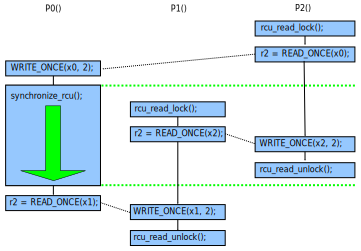
\includegraphics{memorder/RCU1G2R}}
\caption{Cycle for One RCU Grace Period and Two RCU Readers}
\label{fig:memorder:Cycle for One RCU Grace Period and Two RCU Readers}
\end{figure*}

\begin{figure*}[tbp]
\centering
\resizebox{\textwidth}{!}{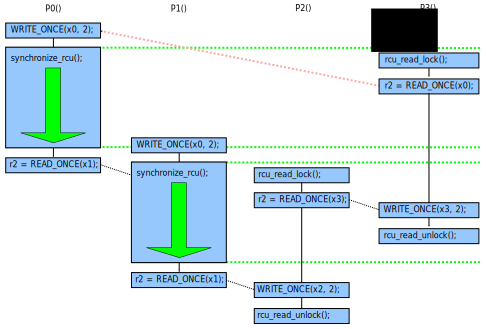
\includegraphics{memorder/RCU2G2R}}
\caption{No Cycle for Two RCU Grace Periods and Two RCU Readers}
\label{fig:memorder:No Cycle for Two RCU Grace Periods and Two RCU Readers}
\end{figure*}

\subsubsection{RCU and Other Ordering Mechanisms}
\label{sec:memorder:RCU and Other Ordering Mechanisms}

But what about litmus tests that combine RCU with other ordering
mechanisms?

The general rule is that it takes only one mechanism to forbid a cycle.

For example, refer back to
\cref{lst:memorder:RCU Readers Provide No Lock-Like Ordering}.
Applying the general rule from the previous section, because this litmus
test has two RCU read-side critical sections and no RCU grace periods,
the cycle is allowed.
But what if \co{P0()}'s \co{WRITE_ONCE()} is replaced by an
\co{smp_store_release()} and \co{P1()}'s \co{READ_ONCE()} is replaced
by an \co{smp_load_acquire()}?

RCU would still allow the cycle, but the release-acquire pair would
forbid it.
Because it only takes one mechanism to forbid a cycle, the
release-acquire pair would ``win'' and the cycle would be
forbidden.

For another example, refer back to
\cref{lst:memorder:One RCU Grace Period and Two Readers}.
Because this litmus test has two RCU readers but only one grace period,
its cycle is allowed.
But suppose that an \co{smp_mb()} was placed between \co{P1()}'s
pair of accesses.
In this new litmus test, because of the addition of the \co{smp_mb()},
\co{P2()}'s as well as \co{P1()}'s critical sections would extend beyond the
end of \co{P0()}'s grace period, which in turn would prevent \co{P2()}'s
read from \co{x0} from preceding \co{P0()}'s write, as depicted by the
red dashed arrow.
In this case, RCU and the full memory barrier work together to forbid
the cycle, with RCU preserving ordering between \co{P0()} and both
\co{P1()} and \co{P2()}, and with the \co{smp_mb()} preserving
ordering between \co{P1()} and \co{P2()}.

\QuickQuiz{}
	What would happen if the \co{smp_mb()} was instead added between
	\co{P2()}'s accesses in
	\cref{lst:memorder:One RCU Grace Period and Two Readers}?
\QuickQuizAnswer{
	The cycle would again be forbidden.
	Further analysis is left as an exercise for the reader.
} \QuickQuizEnd

In short, where RCU's semantics were once purely pragmatic, they are
now fully
formalized~\cite{PaulMcKenney2005RCUSemantics,MathieuDesnoyers2012URCU,AlexeyGotsman2013ESOPRCU,Alglave:2018:FSC:3173162.3177156}.

% \subsection{SRCU}
% \label{sec:memorder:SRCU}
% @@@ After LWN article

% Nesting vs. value passed from \co{srcu_read_lock()} to
% \co{srcu_read_unlock()}.

% When augmented by \co{smp_mb__after_srcu_read_unlock()}.

It is hoped that detailed semantics for higher-level primitives will
enable more capable static analysis and model checking, at least compared
to what can be done based on individual memory accesses.

\section{Hardware Specifics}
\label{sec:memorder:Hardware Specifics}
\OriginallyPublished{Section}{sec:memorder:Hardware Specifics}{Memory-Barrier Instructions For Specific CPUs}{Linux Journal}{PaulMcKenney2005i,PaulMcKenney2005j}

\begin{table*}[tbh]
\rowcolors{4}{}{lightgray}
\small
\centering
\newcommand{\cpufml}[1]{\begin{picture}(6,50)(0,0)\rotatebox{90}{#1}\end{picture}}
\renewcommand*{\arraystretch}{1.2}\OneColumnHSpace{-.35in}
\begin{tabular}{llccccccccc}
	\toprule
	\multicolumn{2}{l}{~} & \multicolumn{9}{c}{CPU Family} \\
	\cmidrule{3-11}
	\multicolumn{2}{c}{\raisebox{.5ex}{Property}}
	& \cpufml{Alpha}
	& \cpufml{ARMv7-A/R}
	& \cpufml{ARMv8}
	& \cpufml{Itanium}
	& \cpufml{MIPS}
	& \cpufml{\Power{}}
	& \cpufml{SPARC TSO}
	& \cpufml{x86}
	& \cpufml{z~Systems}
	\\
	\cmidrule(r){1-2} \cmidrule{3-11}
%		 Alpha ARMv8 ARMv7 Itanium MIPS PPC SPARC x86 z Systems
\cellcolor{white}
	Memory Ordering
	& Loads Reordered After Loads or Stores?
		 & Y   & Y   & Y   & Y     & Y  & Y & ~   & ~ & ~ \\
	& Stores Reordered After Stores?
		 & Y   & Y   & Y   & Y     & Y  & Y & ~   & ~ & ~ \\
\cellcolor{white}
	& Stores Reordered After Loads?
		 & Y   & Y   & Y   & Y     & Y  & Y & Y   & Y & Y \\
	& \parbox[c][6ex]{2in}{\raggedright Atomic Instructions Reordered With\par Loads or Stores?}
		 & Y   & Y   & Y   & ~     & Y  & Y & ~   & ~ & ~ \\
\cellcolor{white}
	& Dependent Loads Reordered?
		 & Y   & ~   & ~   & ~     & ~  & ~ & ~   & ~ & ~ \\
	& Dependent Stores Reordered?
		 & ~   & ~   & ~   & ~     & ~  & ~ & ~   & ~ & ~ \\
\cellcolor{white}
	& Non-Sequentially Consistent?
		 & Y   & Y   & Y   & Y     & Y  & Y & Y   & Y & Y \\
	& Non-Multicopy Atomic?
		 & Y   & Y   & Y   & Y     & Y  & Y & Y   & Y & ~ \\
\cellcolor{white}
	& Non-Other-Multicopy Atomic?
		 & Y   & Y   & ~   & Y     & Y  & Y & ~   & ~ & ~ \\
	& Non-Cache Coherent?
		 & ~   & ~   & ~   & Y     & ~  & ~ & ~   & ~ & ~ \\
	\cmidrule(r){1-2} \cmidrule{3-11}
\cellcolor{white}
	Instructions
	& Load-Acquire/Store-Release?
		 & F   & F   & i   & I     & F  & b & ~   & ~ & ~ \\
	& Atomic RMW Instruction Type?
		 & L   & L   & L   & C     & L  & L & C   & C & C \\
\cellcolor{white}
	& Incoherent Instruction Cache/Pipeline?
		 & Y   & Y   & Y   & Y     & Y  & Y & Y   & Y & Y \\
	\bottomrule
\end{tabular}

\vspace{5pt}\hfill
\framebox[\width]{\footnotesize\setlength{\tabcolsep}{3pt}
\rowcolors{1}{}{}
\renewcommand*{\arraystretch}{1}
\begin{tabular}{llcl}
	{ \bf Key: }
	  & \multicolumn{3}{l}{Load-Acquire/Store-Release?} \\
	~ & ~ & b: & Lightweight memory barrier \\
	~ & ~ & F: & Full memory barrier \\
	~ & ~ & i: & Instruction with lightweight ordering \\
	~ & ~ & I: & Instruction with heavyweight ordering \\
	~ &\multicolumn{3}{l}{Atomic RMW Instruction Type?} \\
	~ & ~ & C: & Compare-and-exchange instruction \\
	~ & ~ & L: & Load-linked/store-conditional instruction \\
\end{tabular}
}\OneColumnHSpace{-0.4in}
\caption{Summary of Memory Ordering}
\label{tab:memorder:Summary of Memory Ordering}
\end{table*}

Each CPU has its own peculiar approach to memory ordering, which
can make portability a challenge, as indicated by
\cref{tab:memorder:Summary of Memory Ordering}.
In fact, some software environments simply prohibit
direct use of memory-ordering operations, restricting the programmer
to mutual-exclusion primitives that incorporate them to the extent that
they are required.  Please note that this section is not intended to be
a reference manual
covering all (or even most) aspects of each CPU family, but rather
a high-level overview giving a rough comparison.
For full details, see the reference manual for the CPU of interest.

Getting back to
\cref{tab:memorder:Summary of Memory Ordering},
the first group of rows look at memory-ordering
properties and the second group looks at instruction properties.

The first three rows indicate whether a given CPU allows the four
possible combinations of loads and stores to be reordered, as discussed
in
\cref{sec:memorder:Ordering: Why and How?} and
\crefrange{sec:memorder:Load Followed By Load}{sec:memorder:Store Followed By Store}.
The next row (``Atomic Instructions Reordered With Loads or Stores?'')
indicates whether a given CPU allows loads and stores
to be reordered with atomic instructions.

The fifth and sixth rows cover reordering and dependencies,
which was covered in
\crefrange{sec:memorder:Address Dependencies}{sec:memorder:Control Dependencies}
and which is explained in more detail in
\cref{sec:memorder:Alpha}.
The short version is that Alpha requires memory barriers for readers
as well as updaters of linked data structures, however, these memory
barriers are provided by the Alpha architecture-specific code in
v4.15 and later Linux kernels.

The next row, ``Non-Sequentially Consistent'', indicates whether
the CPU's normal load and store instructions are constrained by
sequential consistency.
Almost all are not constrained in this way for performance reasons.

The next two rows cover multicopy atomicity, which was defined in
\cref{sec:memorder:Multicopy Atomicity}.
The first is full-up (and rare) multicopy atomicity, and the second is the
weaker other-multicopy atomicity.

The next row, ``Non-Cache Coherent'', covers accesses from multiple
threads to a single variable, which was discussed in
\cref{sec:memorder:Cache Coherence}.

The final three rows cover instruction-level choices and issues.
The first row indicates how each CPU implements load-acquire
and store-release, the second row classifies CPUs by atomic-instruction
type, and the third and final row
indicates whether a given CPU has an incoherent
instruction cache and pipeline.
Such CPUs require special instructions be executed for self-modifying
code.

%Parenthesized CPU names indicate modes that are architecturally allowed,
%but rarely used in practice.

The common ``just say no'' approach to memory-ordering operations
can be eminently reasonable where it applies,
but there are environments, such as the Linux kernel, where direct
use of memory-ordering operations is required.
Therefore,
Linux provides a carefully chosen least-common-denominator
set of memory-ordering primitives, which are as follows:
\begin{description}
\item	[\tco{smp_mb()}] (full memory barrier) that orders both loads and
	stores.
	This means that loads and stores preceding the memory barrier
	will be committed to memory before any loads and stores
	following the memory barrier.
\item	[\tco{smp_rmb()}] (read memory barrier) that orders only loads.
\item	[\tco{smp_wmb()}] (write memory barrier) that orders only stores.
\item	[\tco{smp_read_barrier_depends()}] that forces subsequent operations
	that depend on prior operations to be ordered.
	This primitive is a no-op on all platforms except Alpha, but
	is normally not used directly, but rather as part of
	something like \co{READ_ONCE()} or \co{rcu_dereference()}.
\item	[\tco{smp_mb__before_atomic()}] that forces ordering of accesses
	preceding the \co{smp_mb__before_atomic()} against accesses following
	a later RMW atomic operation.
	This is a noop on systems that fully order atomic RMW operatings.
\item	[\tco{smp_mb__after_atomic()}] that forces ordering of accesses
	preceding an earlier RMW atomic operation against accesses
	following the \co{smp_mb__after_atomic()}.
	This is also a noop on systems that fully order atomic RMW operatings.
\item	[\tco{mmiowb()}] that forces ordering on MMIO writes that are guarded
	by global spinlocks, and is more thoroughly described
	in a 2016 LWN article on MMIO~\cite{PaulEMcKenney2016LinuxKernelMMIO}.
\end{description}
The \co{smp_mb()}, \co{smp_rmb()}, and \co{smp_wmb()}
primitives also force
the compiler to eschew any optimizations that would have the effect
of reordering memory optimizations across the barriers.
The \co{smp_read_barrier_depends()} primitive has a similar effect, but
only on Alpha CPUs.

These primitives generate code only in SMP kernels, however, several
have UP versions ({\tt mb()}, {\tt rmb()}, {\tt wmb()},
and \co{read_barrier_depends()},
respectively) that generate a memory barrier even in UP kernels. The \co{smp_}
versions should be used in most cases. However, these latter primitives
are useful when writing drivers, because MMIO accesses must remain
ordered even in UP kernels. In absence of memory-ordering operations,
both CPUs and compilers would happily rearrange these accesses, which at
best would make the device act strangely, and could crash your kernel or,
in some cases, even damage your hardware.

So most kernel programmers need not worry about the memory-ordering
peculiarities of each and every CPU, as long as they stick to these
interfaces.
If you are working deep in a given CPU's architecture-specific code,
of course, all bets are off.

Furthermore,
all of Linux's locking primitives (spinlocks, reader-writer locks,
semaphores, RCU, \ldots) include any needed ordering primitives.
So if you are working with code that uses these primitives properly,
you need not worry about Linux's memory-ordering primitives.

That said, deep knowledge of each CPU's memory-consistency model
can be very helpful when debugging, to say nothing of when writing
architecture-specific code or synchronization primitives.

Besides, they say that a little knowledge is a very dangerous thing.
Just imagine the damage you could do with a lot of knowledge!
For those who wish to understand more about individual CPUs'
memory consistency models, the next sections describe those of a few
popular and prominent CPUs.
Although nothing can replace actually reading a given CPU's documentation,
these sections give a good overview.

\subsection{Alpha}
\label{sec:memorder:Alpha}

It may seem strange to say much of anything about a CPU whose end of life
has long since past, but Alpha is interesting because it is the only
mainstream CPU that reorders dependent loads, and has thus had outsized
influence on concurrency APIs, including within the Linux kernel.
Understanding Alpha is therefore surprisingly important to the Linux kernel
hacker.

\begin{lineref}[ln:memorder:Insert and Lock-Free Search (No Ordering)]
The dependent-load difference between Alpha and the other CPUs is
illustrated by the code shown in
\cref{lst:memorder:Insert and Lock-Free Search (No Ordering)}.
This \co{smp_wmb()} on \clnref{wmb} of this listing
guarantees that the element initialization
in \clnrefrange{init:b}{init:e} is executed before the element is added to the
list on \clnref{add}, so that the lock-free search will work correctly.
That is, it makes this guarantee on all CPUs {\em except} Alpha.\footnote{
	But Linux kernel versions v4.15 and later cause \co{READ_ONCE()}
	to emit a memory barrier on Alpha, so this discussion applies
	only to older versions of the Linux kernel.}
\end{lineref}

\begin{listing}[tbp]
\begin{linelabel}[ln:memorder:Insert and Lock-Free Search (No Ordering)]
\begin{VerbatimL}[commandchars=\\\[\]]
struct el *insert(long key, long data)
{
	struct el *p;
	p = kmalloc(sizeof(*p), GFP_ATOMIC);
	spin_lock(&mutex);
	p->next = head.next;		\lnlbl[init:b]
	p->key = key;
	p->data = data;			\lnlbl[init:e]
	smp_wmb();			\lnlbl[wmb]
	head.next = p;			\lnlbl[add]
	spin_unlock(&mutex);
}

struct el *search(long key)
{
	struct el *p;
	p = READ_ONCE(head.next);	\lnlbl[h:next]
	while (p != &head) {
		/* Prior to v4.15, BUG ON ALPHA!!! */ \lnlbl[BUG]
		if (p->key == key) {	\lnlbl[key]
			return (p);
		}
		p = READ_ONCE(p->next);	\lnlbl[next]
	};
	return (NULL);
}
\end{VerbatimL}
\end{linelabel}
\caption{Insert and Lock-Free Search (No Ordering)}
\label{lst:memorder:Insert and Lock-Free Search (No Ordering)}
\end{listing}

\begin{lineref}[ln:memorder:Insert and Lock-Free Search (No Ordering)]
Alpha actually allows the code on \clnref{key} of
\cref{lst:memorder:Insert and Lock-Free Search (No Ordering)}
could see the old
garbage values that were present before the initialization on
\clnrefrange{init:b}{init:e}.

\Cref{fig:memorder:Why smp-read-barrier-depends() is Required}
shows how this can happen on
an aggressively parallel machine with partitioned caches, so that
alternating cache lines are processed by the different partitions
of the caches.
For example, the load of \co{head.next} on \clnref{h:next} of
\cref{lst:memorder:Insert and Lock-Free Search (No Ordering)}
might access cache bank~0,
and the load of \co{p->key} on \clnref{key} and of \co{p->next} on \clnref{next}
might access cache bank~1.
On Alpha, the \co{smp_wmb()} will guarantee that the cache invalidations
performed by \clnrefrange{init:b}{init:e} of
\cref{lst:memorder:Insert and Lock-Free Search (No Ordering)}
(for \co{p->next}, \co{p->key}, and \co{p->data}) will reach
the interconnect before that of \clnref{add} (for \co{head.next}), but
makes absolutely no guarantee about the order of
propagation through the reading CPU's cache banks.
For example, it is possible that the reading CPU's cache bank~1 is very
busy, but cache bank~0 is idle.
This could result in the cache invalidations for the new element
(\co{p->next}, \co{p->key}, and \co{p->data}) being
delayed, so that the reading CPU loads the new value for \co{head.next},
but loads the old cached values for \co{p->key} and \co{p->next}.
Yes, this does mean that Alpha can in effect fetch
the data pointed to {\em before} it fetches the pointer itself, strange
but true.
\end{lineref}
See the documentation~\cite{Compaq01,WilliamPugh2000Gharachorloo}
called out earlier for more information,
or if you think that I am just making all this up.\footnote{
	Of course, the astute reader will have already recognized that
	Alpha is nowhere near as mean and nasty as it could be,
	the (thankfully) mythical architecture in
	\cref{sec:app:whymb:Ordering-Hostile Architecture}
	being a case in point.}
The benefit of this unusual approach to ordering is that Alpha can use
simpler cache hardware, which in turn permitted higher clock frequency
in Alpha's heyday.

\begin{figure}[tbp]
\centering
\resizebox{\twocolumnwidth}{!}{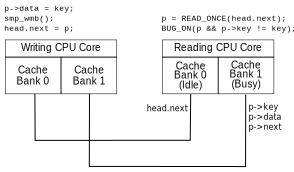
\includegraphics{memorder/Alpha}}
\caption{Why \tco{smp_read_barrier_depends()} is Required}
\label{fig:memorder:Why smp-read-barrier-depends() is Required}
\end{figure}

One could place an \co{smp_rmb()} primitive
between the pointer fetch and dereference in order to force Alpha
to order the pointer fetch with the later dependent load.
However, this imposes unneeded overhead on systems (such as ARM,
Itanium, PPC, and SPARC) that respect data dependencies on the read side.
A \co{smp_read_barrier_depends()} primitive has therefore been added to the
Linux kernel to eliminate overhead on these systems, and was also added
to \co{READ_ONCE()} in v4.15 of the Linux kernel so that core kernel
code no longer needs to concern itself with this aspect of DEC Alpha.
\begin{lineref}[ln:memorder:Insert and Lock-Free Search (No Ordering)]
This \co{smp_read_barrier_depends()} primitive could be inserted in
place of \clnref{BUG} of
\cref{lst:memorder:Insert and Lock-Free Search (No Ordering)},
\end{lineref}
\begin{lineref}[ln:memorder:Safe Insert and Lock-Free Search]
but it is better to use the \co{rcu_dereference()} wrapper macro
as shown on \clnref{deref1,deref2} of
\cref{lst:memorder:Safe Insert and Lock-Free Search}.
\end{lineref}

It is also possible to implement a software mechanism
that could be used in place of \co{smp_wmb()} to force
all reading CPUs to see the writing CPU's writes in order.
This software barrier could be implemented by sending inter-processor
interrupts (IPIs) to all other CPUs.
Upon receipt of such an IPI, a CPU would execute a memory-barrier
instruction, implementing a memory-barrier shootdown similar to that
provided by the Linux kernel's \co{sys_membarrier()} system call.
Additional logic is required to avoid deadlocks.
Of course, CPUs that respect data dependencies would define such a barrier
to simply be \co{smp_wmb()}.
However, this approach was deemed by the Linux community
to impose excessive overhead, and furthermore would
not be considered a reasonable approach by those whose systems must meet
aggressive real-time response requirements.

\begin{listing}[tbp]
\begin{linelabel}[ln:memorder:Safe Insert and Lock-Free Search]
\begin{VerbatimL}[commandchars=\\\[\]]
struct el *insert(long key, long data)
{
	struct el *p;
	p = kmalloc(sizeof(*p), GFP_ATOMIC);
	spin_lock(&mutex);
	p->next = head.next;
	p->key = key;
	p->data = data;
	smp_wmb();
	head.next = p;
	spin_unlock(&mutex);
}

struct el *search(long key)
{
	struct el *p;
	p = rcu_dereference(head.next);		\lnlbl[deref1]
	while (p != &head) {
		if (p->key == key) {
			return (p);
		}
		p = rcu_dereference(p->next);	\lnlbl[deref2]
	};
	return (NULL);
}
\end{VerbatimL}
\end{linelabel}
\caption{Safe Insert and Lock-Free Search}
\label{lst:memorder:Safe Insert and Lock-Free Search}
\end{listing}

The Linux memory-barrier primitives took their names from the Alpha
instructions, so \co{smp_mb()} is {\tt mb}, \co{smp_rmb()} is {\tt rmb},
and \co{smp_wmb()} is {\tt wmb}.
Alpha is the only CPU where \co{smp_read_barrier_depends()} is
an \co{smp_mb()} rather than a no-op.

\QuickQuiz{}
	Why is Alpha's \co{smp_read_barrier_depends()} an
	\co{smp_mb()} rather than \co{smp_rmb()}?
\QuickQuizAnswer{
	Alpha has only \co{mb} and \co{wmb} instructions,
	so \co{smp_rmb()} would be implemented by the Alpha \co{mb}
	instruction in either case.
	In addition, at the time that \co{smp_read_barrier_depends()}
	was added to the Linux kernel, it was not clear that
	Alpha ordered dependent stores, and thus \co{smp_mb()}
	was therefore the safe choice.

	However, v4.15 of the Linux kernel has added
	\co{smp_read_barrier_depends()} to \co{READ_ONCE()} and a few
	of Alpha's atomic read-modify-write operations, thus making it
	unnecessary to use \co{smp_read_barrier_depends()} anywhere else
	in the core kernel.
	This means that other than \co{READ_ONCE()}, no Linux-kernel
	core code need concern itself with DEC Alpha, thus greatly reducing
	Paul E.~McKenney's incentive to remove Alpha support from the
	kernel.
} \QuickQuizEnd

\QuickQuiz{}
	Isn't DEC Alpha significant as having the weakest possible
	memory ordering?
\QuickQuizAnswer{
	Although DEC Alpha does take considerable flak, it does avoid
	reordering reads from the same CPU to the same variable.
	It also avoids the out-of-thin-air problem that plagues
	the Java and C11 memory
	models~\cite{Boehm:2014:OGA:2618128.2618134,conf/esop/BattyMNPS15,MarkBatty2013OOTA-WorkingNote,AlanJeffrey2014JavaDRF,PaulEMcKenney2016OOTA,Sevcik:2011:SOS:1993316.1993534,Vafeiadis:2015:CCO:2775051.2676995}.
} \QuickQuizEnd

For more on Alpha, see its reference manual~\cite{ALPHA2002}.

\subsection{ARMv7-A/R}
\label{sec:memorder:ARMv7-A/R}

The ARM family of CPUs is extremely popular in embedded applications,
particularly for power-constrained applications such as cellphones.
Its memory model is similar to that of \Power{}
(see \cref{sec:memorder:POWER / PowerPC}), but ARM uses a
different set of memory-barrier instructions~\cite{ARMv7A:2010}:

\begin{description}
\item	[\tco{DMB}] (data memory barrier) causes the specified type of
	operations to \emph{appear} to have completed before any
	subsequent operations of the same type.
	The ``type'' of operations can be all operations or can be
	restricted to only writes (similar to the Alpha \co{wmb}
	and the \Power{} \co{eieio} instructions).
	In addition, ARM allows cache coherence to have one of three
	scopes: single processor, a subset of the processors
	(``inner'') and global (``outer'').
\item	[\tco{DSB}] (data synchronization barrier) causes the specified
	type of operations to actually complete before any subsequent
	operations (of any type) are executed.
	The ``type'' of operations is the same as that of \co{DMB}.
	The \co{DSB} instruction was called \co{DWB} (drain write buffer
	or data write barrier, your choice) in early versions of the
	ARM architecture.
\item	[\tco{ISB}] (instruction synchronization barrier) flushes the CPU
	pipeline, so that all instructions following the \co{ISB}
	are fetched only after the \co{ISB} completes.
	For example, if you are writing a self-modifying program
	(such as a JIT), you should execute an \co{ISB} between
	generating the code and executing it.
\end{description}

None of these instructions exactly match the semantics of Linux's
\co{rmb()} primitive, which must therefore be implemented as a full
\co{DMB}.
The \co{DMB} and \co{DSB} instructions have a recursive definition
of accesses ordered before and after the barrier, which has an effect
similar to that of \Power{}'s cumulativity, both of which are
stronger than
\cref{sec:memorder:Cumulativity}'s
variant of cumulativity.

ARM also implements control dependencies, so that if a conditional
branch depends on a load, then any store executed after that conditional
branch will be ordered after the load.
However, loads following the conditional branch will \emph{not}
be guaranteed to be ordered unless there is an \co{ISB}
instruction between the branch and the load.
Consider the following example:

\begin{linelabel}[ln:memorder:ARM:load-store control dependency]
\begin{VerbatimN}[commandchars=\\\[\]]
r1 = x;			\lnlbl[x]
if (r1 == 0)		\lnlbl[if]
	nop();		\lnlbl[nop]
y = 1;			\lnlbl[y]
r2 = z;			\lnlbl[z1]
ISB();			\lnlbl[isb]
r3 = z;			\lnlbl[z2]
\end{VerbatimN}
\end{linelabel}

\begin{lineref}[ln:memorder:ARM:load-store control dependency]
In this example, load-store control dependency ordering causes
the load from \co{x} on \clnref{x} to be ordered before the store to
\co{y} on \clnref{y}.
However, ARM does not respect load-load control dependencies, so that
the load on \clnref{x} might well happen \emph{after} the
load on \clnref{z1}.
On the other hand, the combination of the conditional branch on \clnref{if}
and the \co{ISB} instruction on \clnref{isb} ensures that
the load on \clnref{z2} happens after the load on \clnref{x}.
Note that inserting an additional \co{ISB} instruction somewhere between
\clnref{nop,y} would enforce ordering between \clnref{x,z1}.
\end{lineref}

\subsection{ARMv8}

\begin{figure}[tb]
\centering
\resizebox{2in}{!}{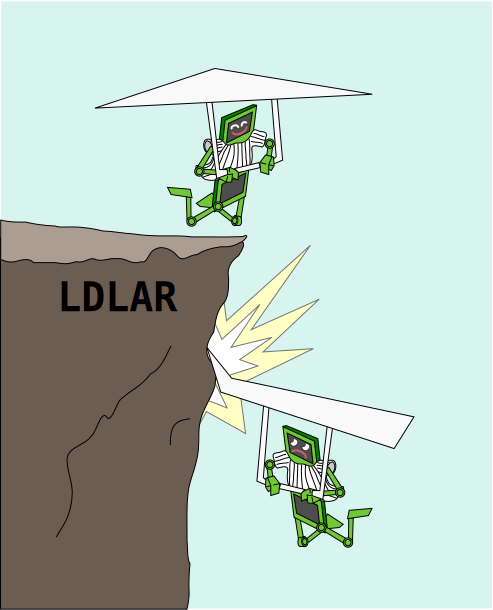
\includegraphics{cartoons/r-2014-LDLAR}}
\caption{Half Memory Barrier}
\ContributedBy{Figure}{fig:memorder:Half Memory Barrier}{Melissa Brossard}
\end{figure}

ARMv8 is ARM's new CPU family~\cite{ARMv8A:2017}
which includes 64-bit capabilities,
in contrast to their 32-bit-only CPU described in
\cref{sec:memorder:ARMv7-A/R}.
ARMv8's memory model closely resembles its ARMv7 counterpart,
but adds load-acquire (\co{LDLARB}, \co{LDLARH}, and \co{LDLAR})
and store-release (\co{STLLRB}, \co{STLLRH}, and \co{STLLR})
instructions.
These instructions act as ``half memory barriers'', so that
ARMv8 CPUs can reorder previous accesses with a later \co{LDLAR}
instruction, but are prohibited from reordering an earlier \co{LDLAR}
instruction with later accesses, as fancifully depicted in
\cref{fig:memorder:Half Memory Barrier}.
Similarly, ARMv8 CPUs can reorder an earlier \co{STLLR} instruction with
a subsequent access, but are prohibited from reordering
previous accesses with a later \co{STLLR} instruction.
As one might expect, this means that these instructions directly support
the C11 notion of load-acquire and store-release.

However, ARMv8 goes well beyond the C11 memory model by mandating that
the combination of a store-release and load-acquire act as a full
barrier under many circumstances.
For example, in ARMv8, given a store followed by a store-release followed
a load-acquire followed by a load, all to different variables and all from
a single CPU, all CPUs
would agree that the initial store preceded the final load.
Interestingly enough, most TSO architectures (including x86 and the
mainframe) do not make this guarantee, as the two loads could be
reordered before the two stores.

ARMv8 is one of only two architectures that needs the
\co{smp_mb__after_spinlock()} primitive to be a full barrier,
due to its relatively weak lock-acquisition implementation in
the Linux kernel.

ARMv8 also has the distinction of being the first CPU whose vendor publicly
defined its memory ordering with an executable formal model~\cite{ARMv8A:2017}.

\subsection{Itanium}
\label{sec:memorder:Itanium}

Itanium offers a weak consistency model, so that in absence of explicit
memory-barrier instructions, Itanium is within its rights to arbitrarily
reorder memory references~\cite{IntelItanium02v2}.
Itanium has a memory-fence instruction named {\tt mf}, but also has
``half-memory fence'' modifiers to loads, stores, and to some of its atomic
instructions~\cite{IntelItanium02v3}.
The {\tt acq} modifier prevents subsequent memory-reference instructions
from being reordered before the {\tt acq}, but permits
prior memory-reference instructions to be reordered after the {\tt acq},
similar to the ARMv8 load-acquire instructions.
Similarly, the {\tt rel} modifier prevents prior memory-reference
instructions from being reordered after the {\tt rel}, but allows
subsequent memory-reference instructions to be reordered before
the {\tt rel}.

These half-memory fences are useful for critical sections, since
it is safe to push operations into a critical section, but can be
fatal to allow them to bleed out.
However, as one of the few CPUs with this property, Itanium at one
time defined Linux's semantics of memory ordering associated with lock
acquisition and release.\footnote{
	PowerPC is now the architecture having this dubious privilege.}
Oddly enough, actual Itanium hardware is rumored to implement
both load-acquire and store-release instructions as full barriers.
Nevertheless, Itanium was the first mainstream CPU to introduce the concept
(if not the reality) of load-acquire and store-release into its
instruction set.

The Itanium {\tt mf} instruction is used for the \co{smp_rmb()},
\co{smp_mb()}, and \co{smp_wmb()} primitives in the Linux kernel.
Oh, and despite rumors to the contrary, the ``mf'' mnemonic really
does stand for ``memory fence''.

Itanium also offers a global total order for ``release'' operations,
including the ``mf'' instruction.
This provides the notion of transitivity, where if a given code fragment
sees a given access as having happened, any later code fragment will
also see that earlier access as having happened.
Assuming, that is, that all the code fragments involved correctly use
memory barriers.

Finally, Itanium is the only architecture supporting the Linux kernel
that can reorder normal loads to the same variable.
The Linux kernel avoids this issue because \co{READ_ONCE()} emits
a \co{volatile} load, which is compiled as a \co{ld,acq} instruction,
which forces ordering of all \co{READ_ONCE()} invocations by a given
CPU, including those to the same variable.

\subsection{MIPS}

The MIPS memory model~\cite[page~479]{MIPSvII-A-2017}
appears to resemble that of ARM, Itanium, and \Power{},
being weakly ordered by default, but respecting dependencies.
MIPS has a wide variety of memory-barrier instructions, but ties them
not to hardware considerations, but rather to the use cases provided
by the Linux kernel and the C++11 standard~\cite{RichardSmith2015N4527}
in a manner similar to the ARMv8 additions:

\begin{description}[style=nextline]
\item[\tco{SYNC}]
	Full barrier for a number of hardware operations in addition
	to memory references, which is used to implement the v4.13
	Linux kernel's \co{smp_mb()} for OCTEON systems.
\item[\tco{SYNC_WMB}]
	Write memory barrier, which can be used on OCTEON systems
	to implement the
	\co{smp_wmb()} primitive in the v4.13 Linux kernel via the
	\co{syncw} mnemonic.
	Other systems use plain \co{sync}.
\item[\tco{SYNC_MB}]
	Full memory barrier, but only for memory operations.
	This may be used to implement the 
	C++ \co{atomic_thread_fence(memory_order_seq_cst)}.
\item[\tco{SYNC_ACQUIRE}]
	Acquire memory barrier, which could be used to implement
	C++'s \co{atomic_thread_fence(memory_order_acquire)}.
	In theory, it could also be used to implement the v4.13 Linux-kernel
	\co{smp_load_acquire()} primitive, but in practice
	\co{sync} is used instead.
\item[\tco{SYNC_RELEASE}]
	Release memory barrier, which may be used to implement
	C++'s \co{atomic_thread_fence(memory_order_release)}.
	In theory, it could also be used to implement the v4.13 Linux-kernel
	\co{smp_store_release()} primitive, but in practice
	\co{sync} is used instead.
\item[\tco{SYNC_RMB}]
	Read memory barrier, which could in theory be used to implement the
	\co{smp_rmb()} primitive in the Linux kernel, except that current
	MIPS implementations supported by the v4.13 Linux kernel do not
	need an explicit instruction to force ordering.
	Therefore, \co{smp_rmb()} instead simply constrains the compiler.
\item[\tco{SYNCI}]
	Instruction-cache synchronization, which is used in conjunction with
	other instructions to allow self-modifying code, such as that produced
	by just-in-time (JIT) compilers.
\end{description}

Informal discussions with MIPS architects indicates that MIPS has a
definition of transitivity or cumulativity similar to that of
ARM and \Power{}.
However, it appears that different MIPS implementations can have
different memory-ordering properties, so it is important to consult
the documentation for the specific MIPS implementation you are using.

\subsection{\Power{} / PowerPC}
\label{sec:memorder:POWER / PowerPC}

The \Power{} and PowerPC\mytextregistered\
CPU families have a wide variety of memory-barrier
instructions~\cite{PowerPC94,MichaelLyons05a}:
\begin{description}
\item	[\tco{sync}] causes all preceding operations to {\em appear to have}
	completed before any subsequent operations are started.
	This instruction is therefore quite expensive.
\item	[\tco{lwsync}] (lightweight sync) orders loads with respect to
	subsequent loads and stores, and also orders stores.
	However, it does {\em not} order stores with respect to subsequent
	loads.
	The \co{lwsync} instruction may be used to implement
	load-acquire and store-release operations.
	Interestingly enough, the {\tt lwsync} instruction enforces
	the same within-CPU ordering as does x86, z~Systems, and coincidentally,
	SPARC TSO.
	However, placing the \co{lwsync} instruction between each
	pair of memory-reference instructions will \emph{not}
	result in x86, z~Systems, or SPARC TSO memory ordering.
	On these other systems, if a pair of CPUs independently execute
	stores to different variables, all other CPUs will agree on the
	order of these stores.
	Not so on PowerPC, even with an \co{lwsync} instruction between each
	pair of memory-reference instructions, because PowerPC is
	non-multicopy atomic.
\item	[\tco{eieio}] (enforce in-order execution of I/O, in case you
	were wondering) causes all preceding cacheable stores to appear
	to have completed before all subsequent stores.
	However, stores to cacheable memory are ordered separately from
	stores to non-cacheable memory, which means that {\tt eieio}
	will not force an MMIO store to precede a spinlock release.
\item	[\tco{isync}] forces all preceding instructions to appear to have
	completed before any subsequent instructions start execution.
	This means that the preceding instructions must have progressed
	far enough that any traps they might generate have either happened
	or are guaranteed not to happen, and that any side-effects of
	these instructions (for example, page-table changes) are seen by the
	subsequent instructions.
\end{description}

Unfortunately, none of these instructions line up exactly with Linux's
{\tt wmb()} primitive, which requires {\em all} stores to be ordered,
but does not require the other high-overhead actions of the {\tt sync}
instruction.
But there is no choice: ppc64 versions of {\tt wmb()} and {\tt mb()} are
defined to be the heavyweight {\tt sync} instruction.
However, Linux's \co{smp_wmb()} instruction is never used for MMIO
(since a driver must carefully order MMIOs in UP as well as
SMP kernels, after all), so it is defined to be the lighter weight
\co{eieio} or \co{lwsync} instruction~\cite{PaulEMcKenney2016LinuxKernelMMIO}.
This instruction may well be unique in having a five-vowel mnemonic.
The \co{smp_mb()} instruction is also defined to be the {\tt sync}
instruction, but both \co{smp_rmb()} and \co{rmb()} are defined to
be the lighter-weight {\tt lwsync} instruction.

\Power{} features ``cumulativity'', which can be used to obtain
transitivity.
When used properly, any code seeing the results of an earlier
code fragment will also see the accesses that this earlier code
fragment itself saw.
Much more detail is available from
McKenney and Silvera~\cite{PaulEMcKenneyN2745r2009}.

\Power{} respects control dependencies in much the same way that ARM
does, with the exception that the \Power{} \co{isync} instruction
is substituted for the ARM \co{ISB} instruction.

Like ARMv8, \Power{} requires \co{smp_mb__after_spinlock()} to be
a full memory barrier.
In addition, \Power{} is the only architecture requiring
\co{smp_mb__after_unlock_lock()} to be a full memory barrier.
In both cases, this is because of the weak ordering properties
of \Power{}'s locking primitives, due to the use of the \co{lwsync}
instruction to provide ordering for both acquisition and release.

Many members of the \Power{} architecture have incoherent instruction
caches, so that a store to memory will not necessarily be reflected
in the instruction cache.
Thankfully, few people write self-modifying code these days, but JITs
and compilers do it all the time.
Furthermore, recompiling a recently run program looks just like
self-modifying code from the CPU's viewpoint.
The {\tt icbi} instruction (instruction cache block invalidate)
invalidates a specified cache line from
the instruction cache, and may be used in these situations.

\subsection{SPARC TSO}

Although SPARC's TSO (total-store order) is used by both Linux and
Solaris, the architecture also defines PSO (partial store order) and RMO
(relaxed-memory order).
Any program that runs in RMO will also run in either PSO or TSO, and similarly,
a program that runs in PSO will also run in TSO.
Moving a shared-memory parallel program in the other direction may
require careful insertion of memory barriers.

Although SPARC's PSO and RMO modes are not used much these days, they
did give rise to a very flexible memory-barrier instruction~\cite{SPARC94}
that permits fine-grained control of ordering:
\begin{description}
\item	[\tco{StoreStore}] orders preceding stores before subsequent stores.
	(This option is used by the Linux \co{smp_wmb()} primitive.)
\item	[\tco{LoadStore}] orders preceding loads before subsequent stores.
\item	[\tco{StoreLoad}] orders preceding stores before subsequent loads.
\item	[\tco{LoadLoad}] orders preceding loads before subsequent loads.
	(This option is used by the Linux \co{smp_rmb()} primitive.)
\item	[\tco{Sync}] fully completes all preceding operations before starting
	any subsequent operations.
\item	[\tco{MemIssue}] completes preceding memory operations before subsequent
	memory operations, important for some instances of memory-mapped
	I/O.
\item	[\tco{Lookaside}] does the same as MemIssue,
	but only applies to preceding stores
	and subsequent loads, and even then only for stores and loads that
	access the same memory location.
\end{description}

So, why is \qco{membar #MemIssue} needed?
Because a \qco{membar #StoreLoad} could permit a subsequent
load to get its value from a store buffer, which would be
disastrous if the write was to an MMIO register that induced side effects
on the value to be read.
In contrast, \qco{membar #MemIssue} would wait until the store buffers
were flushed before permitting the loads to execute,
thereby ensuring that the load actually gets its value from the MMIO register.
Drivers could instead use \qco{membar #Sync}, but the lighter-weight
\qco{membar #MemIssue} is preferred in cases where the additional function
of the more-expensive \qco{membar #Sync} are not required.

The \qco{membar #Lookaside} is a lighter-weight version of
\qco{membar #MemIssue}, which is useful when writing to a given MMIO register
affects the value that will next be read from that register.
However, the heavier-weight \qco{membar #MemIssue} must be used when
a write to a given MMIO register affects the value that will next be
read from {\em some other} MMIO register.

SPARC requires a {\tt flush} instruction be used between the time that
an instruction is stored and executed~\cite{SPARC94}.
This is needed to flush any prior value for that location from
the SPARC's instruction cache.
Note that {\tt flush} takes an address, and will flush only that address
from the instruction cache.
On SMP systems, all CPUs' caches are flushed, but there is no
convenient way to determine when the off-CPU flushes complete,
though there is a reference to an implementation note.

But again, the Linux kernel runs SPARC in TSO mode, so
all of the above \co{membar} variants are strictly of historical
interest.
In particular, the \co{smp_mb()} primitive only needs to use \co{#StoreLoad}
because the other three reorderings are prohibited by TSO.

\subsection{x86}

Historically, the x86 CPUs provided ``process ordering'' so that all CPUs
agreed on the order of a given CPU's writes to memory.
This allowed the \co{smp_wmb()}
primitive to be a no-op for the CPU~\cite{IntelXeonV3-96a}.
Of course, a compiler directive was also required to prevent optimizations
that would reorder across the \co{smp_wmb()} primitive.
In ancient times, certain x86 CPUs gave no ordering guarantees for loads, so
the \co{smp_mb()} and \co{smp_rmb()} primitives expanded to {\tt lock;addl}.
This atomic instruction acts as a barrier to both loads and stores.

But those were ancient times.
More recently, Intel has published a memory model for
x86~\cite{Intelx86MemoryOrdering2007}.
It turns out that Intel's modern CPUs enforce tighter ordering than
was claimed in the previous specifications, so this model is in effect
simply mandating this modern behavior.
Even more recently, Intel published an updated memory model for
x86~\cite[Section 8.2]{Intel64IA32v3A2011}, which mandates a total global order
for stores, although individual CPUs are still permitted to see their
own stores as having happened earlier than this total global order
would indicate.
This exception to the total ordering is needed to allow important
hardware optimizations involving store buffers.
In addition, x86 provides other-multicopy atomicity, for example,
so that if CPU~0 sees a store by CPU~1, then CPU~0 is guaranteed to see
all stores that CPU~1 saw prior to its store.
Software may use atomic operations to override these hardware optimizations,
which is one reason that atomic operations tend to be more expensive
than their non-atomic counterparts.

It is also important to note that atomic instructions operating
on a given memory location should all be of the same
size~\cite[Section 8.1.2.2]{Intel64IA32v3A2011}.
For example, if you write a program where one CPU atomically increments
a byte while another CPU executes a 4-byte atomic increment on
that same location, you are on your own.

However, note that some SSE instructions are weakly ordered ({\tt clflush}
and non-temporal move instructions~\cite{IntelXeonV2b-96a}).
Code that uses these non-temporal move instructions
can also use {\tt mfence} for \co{smp_mb()},
{\tt lfence} for \co{smp_rmb()}, and {\tt sfence} for \co{smp_wmb()}.

A few older variants of the x86 CPU have a mode bit that enables out-of-order
stores, and for these CPUs, \co{smp_wmb()} must also be defined to
be {\tt lock;addl}.

Although newer x86 implementations accommodate self-modifying code
without any special instructions, to be fully compatible with
past and potential future x86 implementations, a given CPU must
execute a jump instruction or a serializing instruction (e.g., \co{cpuid})
between modifying the code and executing
it~\cite[Section 8.1.3]{Intel64IA32v3A2011}.

\subsection{z Systems}

The z~Systems machines make up the IBM\mytexttrademark\
mainframe family, previously
known as the 360, 370, 390 and zSeries~\cite{IBMzSeries04a}.
Parallelism came late to z~Systems, but given that these mainframes first
shipped in the mid 1960s, this is not saying much.
The \qco{bcr 15,0} instruction is used for the Linux \co{smp_mb()} primitives,
but compiler constraints suffices for both the
\co{smp_rmb()} and \co{smp_wmb()} primitives.
It also has strong memory-ordering semantics, as shown in
\cref{tab:memorder:Summary of Memory Ordering}.
In particular, all CPUs
will agree on the order of unrelated stores from different CPUs,
that is, z~Systems is fully multicopy atomic.

As with most CPUs, the z~Systems architecture does not guarantee a
cache-coherent instruction stream, hence,
self-modifying code must execute a serializing instruction between updating
the instructions and executing them.
That said, many actual z~Systems machines do in fact accommodate self-modifying
code without serializing instructions.
The z~Systems instruction set provides a large set of serializing instructions,
including compare-and-swap, some types of branches (for example, the
aforementioned \qco{bcr 15,0} instruction), and test-and-set,
among others.

\section{Where is Memory Ordering Needed?}
\label{sec:memorder:Where is Memory Ordering Needed?}

This section revisits
\cref{tab:memorder:Linux-Kernel Memory-Ordering Cheat Sheet}
and \cref{sec:memorder:Basic Rules of Thumb},
summarizing the intervening discussion with a more sophisticated
set of rules of thumb.

The first rule of thumb is that memory-ordering operations are only
required where there is a possibility of interaction involving at least
two variables shared among at least two threads.
In light of the intervening material, this single sentence encapsulates much of
\cref{sec:memorder:Basic Rules of Thumb}'s basic rules of thumb,
for example, keeping in mind that ``memory-barrier pairing'' is a
two-thread special case of ``cycle''.
And, as always, if a single-threaded program will provide sufficient
performance, why bother with parallelism?\footnote{
	Hobbyists and researchers should of course feel free to ignore
	this and other cautions.}
After all, avoiding parallelism also avoids the added cost of
memory-ordering operations.

The second rule of thumb involves load-buffering situations:
If all thread-to-thread communication in a given cycle use store-to-load links
(that is, the next thread's load returning the value that the previous thread
stored), minimal ordering suffices.
Minimal ordering includes dependencies and acquires as well as all stronger
ordering operations.

The third rule of thumb involves release-acquire chains:
If all but one of the links in a given cycle is a store-to-load
link, it is sufficient to use release-acquire pairs for each of
those store-to-load links, as illustrated by
\cref{lst:memorder:Long ISA2 Release-Acquire Chain,%
lst:memorder:Long Z6.2 Release-Acquire Chain}.
You can replace a given acquire with a dependency in environments permitting
this, keeping in mind that the C11 standard's memory model does \emph{not}
fully respect dependencies.
Therefore, a dependency leading to a load must be headed by
a \co{READ_ONCE()} or an \co{rcu_dereference()}:
a plain C-language load is not sufficient.
In addition, never forget to carefully review
\cref{sec:memorder:Address- and Data-Dependency Difficulties,%
sec:memorder:Control-Dependency Calamities}, because
a dependency broken by your compiler is no help at all!
The two threads sharing the sole non-store-to-load link can
usually substitute \co{WRITE_ONCE()} plus \co{smp_wmb()} for
\co{smp_store_release()} on the one hand,
and \co{READ_ONCE()} plus \co{smp_rmb()} for \co{smp_load_acquire()}
on the other.
However, the wise developer will check such substitutions carefully,
for example, using the herd tool as described in
\cref{sec:formal:Axiomatic Approaches}.

\QuickQuiz{}
	Why is it necessary to use heavier-weight ordering for
	load-to-store and store-to-store links, but not for
	store-to-load links?
	What on earth makes store-to-load links so special???
\QuickQuizAnswer{
	Recall that load-to-store and store-to-store links can be
	counter-temporal, as illustrated by
	\cref{fig:memorder:Load-to-Store is Counter-Temporal,%
	fig:memorder:Store-to-Store is Counter-Temporal} in
	\cref{sec:memorder:Propagation}.
	This counter-temporal nature of load-to-store and store-to-store
	links necessitates strong ordering.

	In constrast, store-to-load links are temporal, as illustrated by
	\cref{lst:memorder:Load-Buffering Data-Dependency Litmus Test,%
	lst:memorder:Load-Buffering Control-Dependency Litmus Test}.
	This temporal nature of store-to-load links permits use of
	minimal ordering.
} \QuickQuizEnd

The fourth and final rule of thumb identifies where full memory barriers
(or stronger) are required:
If a given cycle contains two or more non-store-to-load links (that is,
a total of two or more load-to-store and store-to-store links), you will
need at least one full barrier between each pair of non-store-to-load
links in that cycle, as illustrated by
\cref{lst:memorder:W+WRC Litmus Test With More Barriers}
as well as in the answer to
\QuickQuizARef{\MemorderQQLitmusTestR}.
Full barriers include \co{smp_mb()}, successful full-strength non-\co{void}
atomic RMW operations, and other atomic RMW operations in conjunction with
either \co{smp_mb__before_atomic()} or \co{smp_mb__after_atomic()}.
Any of RCU's grace-period-wait primitives (\co{synchronize_rcu()} and
friends) also act as full barriers, but at far greater expense than
\co{smp_mb()}.
With strength comes expense, though full barriers
usually hurt performance more than they hurt scalability.

Note that these four rules of thumb encapsulate \emph{minimum} guarantees.
Different architectures may give
more substantial guarantees,
as discussed in \cref{sec:memorder:Hardware Specifics},
but they may \emph{not}
be relied upon outside of code specifically designed to run only on
the corresponding architecture.
In addition, more involved memory models may give stronger
guarantees~\cite{Alglave:2018:FSC:3173162.3177156}, at the
expense of somewhat greater complexity.

One final word of advice: Use of raw memory-ordering primitives is
a last resort.
It is almost always better to use existing primitives, such as locking
or RCU, thus letting those primitives do the memory ordering for you.
